% 6-10 pages, 9pt font
%
% Topics:
%
% * Machine learning based autotuning.
% * Representative benchmarking.
% * Automatic fault tolerance.
% * Run-time adaption.
%

% The following \documentclass options may be useful:
%
% preprint      Remove this option only once the paper is in final form.
% 10pt          To set in 10-point type instead of 9-point.
% 11pt          To set in 11-point type instead of 9-point.
% authoryear    To obtain author/year citation style instead of numeric.
\documentclass[nonatbib,preprint,9pt]{sigplanconf}

%%%%%%%%%%%%%%%%%%%%%%%%%
%% Document and Layout %%
%%%%%%%%%%%%%%%%%%%%%%%%%

% Fix for multiple "No room for a new \dimen" errors.
%
% See: http://tex.stackexchange.com/questions/38607/no-room-for-a-new-dimen
%
\usepackage{etex}

\usepackage[utf8]{inputenc}

% Fix for "'babel/polyglossia' detected but 'csquotes' missing"
% warning. NOTE: Include after inputenc.
%
\usepackage{csquotes}

% Make internal macro definitions accessible,
% e.g. \@title, \@date \@author.
\makeatletter

% Multi-column support.
\usepackage{multicol}

% A useful package which includes macros like \ifdef{}{}{}:
%
\usepackage{etoolbox}

% Uncomment the following line to remove column separation:
%
%\setlength{\columnsep}{5mm}

% Allow user-defined warning and error filters.
%
\usepackage{silence}


%%%%%%%%%%%%%%%%%%%%%
% Table of Contents %
%%%%%%%%%%%%%%%%%%%%%

% % Set chapter and section numbering depth:
% %
% \setcounter{secnumdepth}{2}


%%%%%%%%%%%%%%%%
% Bibliography %
%%%%%%%%%%%%%%%%
\usepackage[%
    backend=biber,
    style=numeric-comp,
    % style=numeric-comp,  % numerical-compressed
    sorting=none,        % nty,nyt,nyvt,anyt,anyvt,ynt,ydnt,none
    sortcites=true,      % sort \cite{b a d c}: true,false
    block=none,          % space between blocks: none,space,par,nbpar,ragged
    indexing=false,      % indexing options: true,false,cite,bib
    citereset=none,      % don't reset cites
    isbn=false,          % print ISBN?
    url=true,            % print URL?
    doi=false,           % print DOI?
    natbib=true,         % natbib compatability
  ]{biblatex}

% % Filter annoying and unavoidable biblatex warning:
\WarningFilter{biblatex}{Patching footnotes failed}

% Reduce the font size of the bibliography:
% \renewcommand{\bibfont}{\normalfont\scriptsize}

% Determine which BibTeX file to use:
%
% If available, use my Mendeley BibTex library, located in the home
% directory. Note that this is a relative path and will break if
% either this file or the BibTex library are moved. If the library is
% not present, use the local refs.bib file.
\newcommand{\BibResourceGlobal}{../../library.bib}
\newcommand{\BibResourceLocal}{refs.bib}

\IfFileExists{\BibResourceGlobal}
  {\newcommand{\BibResource}{\BibResourceGlobal}}
  {\newcommand{\BibResource}{\BibResourceLocal}}

\addbibresource{\BibResource}


%%%%%%%%%%%%%%
% Appendices %
%%%%%%%%%%%%%%

% Appendix package. Documentation:
%
%  http://mirror.ox.ac.uk/sites/ctan.org/macros/latex/contrib/appendix/appendix.pdf
%
% Package options:
%
% toc      - Put a header (e.g., `Appendices') into the Table of Contents
%            (the ToC) before listing the appendices. (This is done by
%            calling the \addappheadtotoc command.)
% page     - Puts a title (e.g., `Appendices') into the document at the
%            point where the appendices environment is begun. (This is
%            done by calling the \appendixpage command.)
% title    - Adds a name (e.g., `Appendix') before each appendix title in
%            the body of the document. The name is given by the value
%            of \appendixname. Note that this is the default behaviour
%            for classes that have chapters.
% titletoc - Adds a name (e.g., `Appendix') before each appendix listed
%            in the ToC. The name is given by the value
%            of \appendixname.
% header   - Adds a name (e.g., `Appendix') before each appendix in page
%            headers.  The name is given by the value
%            of \appendixname. Note that this is the default behaviour
%            for classes that have chapters.
\usepackage[title, titletoc]{appendix}


%%%%%%%%%%%%%%%%%%%%%%%%%%%%%%%%%%%%%
%% Figures, footnotes and listings %%
%%%%%%%%%%%%%%%%%%%%%%%%%%%%%%%%%%%%%

%\usepackage{float}
%\restylefloat{figure}

% Use bold ``(Figure|Table|Listing)'' caption text.
%\usepackage[margin=1cm]{caption}

% Set the font for captions.
% \renewcommand{\captionfont}{\small}
% Set the font for caption labels.
% \renewcommand{\captionlabelfont}{\footnotesize\bf}

% Use arabic numbers for footnote.
%\renewcommand{\thefootnote}{\arabic{footnote}}

% Ensure that footnotes always appear at the bottom of pages.
%\usepackage[bottom]{footmisc}

% Reset the footnote counter on every page.
%\usepackage{perpage}
%\MakePerPage{footnote}

% Pre-requisites for rendering upquotes in listings package.
\usepackage[T1]{fontenc}
\usepackage{lmodern}
\usepackage{textcomp}

% Pseudo-code listings.
\usepackage{algorithm}
\usepackage{algpseudocode}
\newcommand{\Break}{\State \textbf{break} }
\algblockdefx[Loop]{Loop}{EndLoop}[1][]{\textbf{Loop} #1}{\textbf{End
    Loop}}

\algrenewcommand\ALG@beginalgorithmic{\footnotesize}

% Code listings.
\usepackage{listings}

% Set \ttfamily to use courier fonts.
%
% See: http://tex.stackexchange.com/a/33686
%
\usepackage{courier}

\lstset{frame=bt,                    % Add top and bottom frame lines
        breaklines=true,             % Force line wrapping
        captionpos=b,                % Place caption below listing
        numbers=left,                % Add left-side line numbers
        basicstyle=\scriptsize\ttfamily, % Set font size and type
        showstringspaces=false,      % Don't show visible whitespace
        numberstyle=\tiny,
        upquote=true,                % Use upright quotes, not curly
        commentstyle=\bfseries}      % Embolden comments

% Use (*@ @*) to escape LaTeX commands within listings.
\lstset{escapeinside={(*@}{@*)}}

% Add 10pt space between chapters in TOC listings entries:
%\let\Chapter\chapter
%\def\chapter{\addtocontents{lol}{\protect\addvspace{10pt}}\Chapter}


%%%%%%%%%%%%%%%%%%%%%%%%
%% Graphics and maths %%
%%%%%%%%%%%%%%%%%%%%%%%%
\usepackage{amsmath}

% Vector notation, e.g. \vv{x}:
%
\usepackage{esvect}

% Additional amsmath symbols, see:
%
% http://texblog.org/2007/08/27/number-sets-prime-natural-integer-rational-real-and-complex-in-latex/
%
\usepackage{amsfonts}
\usepackage{amssymb}

\usepackage{graphicx}
\usepackage{mathtools}
\usepackage{tikz}
\usepackage{tikz-qtree}

% Provide bold font face in maths.
\usepackage{bm}

\usepackage{subcaption}
\expandafter\def\csname ver@subfig.sty\endcsname{}

% Define an 'myalignat' command which behave as 'alignat' without the
% vertical top and bottom padding. See:
%     http://www.latex-community.org/forum/viewtopic.php?f=5&t=1890
\newenvironment{myalignat}[1]{%
  \setlength{\abovedisplayskip}{-.7\baselineskip}%
  \setlength{\abovedisplayshortskip}{\abovedisplayskip}%
  \start@align\z@\st@rredtrue#1
}%
{\endalign}

% Define additional operators:
\DeclareMathOperator*{\argmin}{arg\,min}
\DeclareMathOperator*{\argmax}{arg\,max}

\DeclareMathOperator*{\gain}{Gain}

% Skeleton operators.
\DeclareMathOperator*{\map}{Map}
\DeclareMathOperator*{\reduce}{Reduce}
\DeclareMathOperator*{\scan}{Scan}
\DeclareMathOperator*{\stencil}{Stencil}
\DeclareMathOperator*{\zip}{Zip}
\DeclareMathOperator*{\allpairs}{All\,Pairs}

% Maths plots using pgfplots, see:
%
%     http://pgfplots.sourceforge.net/pgfplots.pdf
%
\usepackage{pgfplots}

% Disable compatability mode.
%
\pgfplotsset{compat=1.12}

% Gantt charts using pgfgantt, see:
%
%     http://www.ctan.org/pkg/pgfgantt
%
\usepackage{pgfgantt}

% Fix milestone aspect ratio by defining a custom element.
\newganttchartelement*{mymilestone}{
  mymilestone/.style={
    shape=diamond,
    inner sep=2pt,
    draw=black,
    top color=black,
    bottom color=black,
  }
}

% Tikz flowchart configuration.
\usetikzlibrary{shapes,arrows,shadows,fit,backgrounds}
\tikzstyle{decision} = [diamond,
                        draw,
                        text width=4.5em,
                        text badly centered,
                        node distance=3cm,
                        inner sep=0pt]
\tikzstyle{block}    = [rectangle,
                        draw,
                        text width=5em,
                        text centered,
                        node distance=3cm,
                        minimum height=4em,
                        inner sep=.2cm]
\tikzstyle{line}     = [draw, -latex']

% Add dirtree picture style, see:
%
%     http://tex.stackexchange.com/a/34268
%
\newcount\dirtree@lvl
\newcount\dirtree@plvl
\newcount\dirtree@clvl
\def\dirtree@growth{%
  \ifnum\tikznumberofcurrentchild=1\relax
    \global\advance\dirtree@plvl by 1
    \expandafter\xdef\csname dirtree@p@\the\dirtree@plvl\endcsname{\the\dirtree@lvl}
  \fi
  \global\advance\dirtree@lvl by 1\relax
  \dirtree@clvl=\dirtree@lvl
  \advance\dirtree@clvl by -\csname dirtree@p@\the\dirtree@plvl\endcsname
  \pgf@xa=0.33cm\relax
  \pgf@ya=-\baselineskip\relax
  \pgf@ya=\dirtree@clvl\pgf@ya
  \pgftransformshift{\pgfqpoint{\the\pgf@xa}{\the\pgf@ya}}%
  \ifnum\tikznumberofcurrentchild=\tikznumberofchildren
    \global\advance\dirtree@plvl by -1
  \fi
}
\tikzset{
  dirtree/.style={
    growth function=\dirtree@growth,
    every node/.style={anchor=north},
    every child node/.style={anchor=west},
    edge from parent path={(\tikzparentnode\tikzparentanchor) |- (\tikzchildnode\tikzchildanchor)}
  }
}

% UML sequence diagram macros, see:
%
%     https://code.google.com/p/pgf-umlsd/
%
% Options:
%
%     underline - Underline object names
%
\usepackage[underline=false]{pgf-umlsd}

% Support for SVG graphics.
%
% NOTE that you must pass the "--shell-escape" argument to pdflatex to
% compile. NOTE also that images *MUST* be placed within the graphics
% path.
\usepackage{svg}
\graphicspath{{img/}}

%%%%%%%%%%%%%%%%%%%%%%
%% Tables and lists %%
%%%%%%%%%%%%%%%%%%%%%%

% Required to use labm8 exported tables.
%
\usepackage{booktabs}

% Required for full page-width tables.
\usepackage{tabularx}

%\usepackage{enumitem}
%\setenumerate{itemsep=0pt}

% Use no left margin for lists:
%\setlist{leftmargin=*}

\usepackage{longtable}

% Define column types L, C, R with known text justification and fixed
% widths:
\usepackage{array}
\newcolumntype{L}[1]{>{\raggedright\let\newline\\\arraybackslash\hspace{0pt}}m{#1}}
\newcolumntype{C}[1]{>{\centering\let\newline\\\arraybackslash\hspace{0pt}}m{#1}}
\newcolumntype{R}[1]{>{\raggedleft\let\newline\\\arraybackslash\hspace{0pt}}m{#1}}


%%%%%%%%%%%%%%%%%%%%%%%%%%%%%
%% Typesetting and symbols %%
%%%%%%%%%%%%%%%%%%%%%%%%%%%%%

% Adjustable font sizes in \Verbatim{}
\usepackage{fancyvrb}

%\usepackage{titlesec}
% Set section and paragraph heading fonts:
%\titleformat*{\section}{\Large\bfseries}
%\titleformat*{\subsection}{\normalsize\bfseries}
%\titleformat*{\subsubsection}{\normalsize}
%\titleformat*{\paragraph}{\large\bfseries}
%\titleformat*{\subparagraph}{\large\bfseries}

% Set section heading margins. Usage:
% \titlespacing*{<command>}{<left>}{<before>}{<after>}
%\titlespacing*{\section}{0pt}{.6em}{.3em}
%\titlespacing*{\subsection}{0pt}{.6em}{.2em}

% Set paragraph indentation size. Default is 15pt.
%\setlength{\parindent}{10pt}

% The line spacing can be globally set using \linespread:
%
% \linespread{1.2}

% Add a command \hr{} which will draw a horizontal rule the width of
% the text.
%
\newcommand{\hr}{\noindent\makebox[\linewidth]{\rule{\textwidth}{0.2pt}}}

% Add a command \br{} which will create a horizontal space of exactly
% one line height.
%
\newcommand{\br}{\hspace{\baselineskip}}

% Define a command to allow word breaking.
\newcommand*\wrapletters[1]{\wr@pletters#1\@nil}
\def\wr@pletters#1#2\@nil{#1\allowbreak\if&#2&\else\wr@pletters#2\@nil\fi}

% Define a command to create centred page titles.
\newcommand{\centredtitle}[1]{
  \begin{center}
    \large
    \vspace{0.9cm}
    \textbf{#1}
  \end{center}}

% Support hyperlinks using the \hyperref, \url and \href
% macros. Usage:
%
%    \hyperref[label_name]{''link text''}
%
%    \url{<my_url>}
%
%    \href{<my_url>}{<description>}
%
\usepackage{hyperref}

% Disable colored borders of links, cross-references etc in PDF output
\hypersetup{pdfborder={0 0 0}}

% Provide generic commands \degree, \celsius, \perthousand, \micro
% and \ohm which work both in text and maths mode.
\usepackage{gensymb}

%%%%%%%%%%%%%%%%%%%%%%%%%%%%%%%%%
%% Placeholder text generation %%
%%%%%%%%%%%%%%%%%%%%%%%%%%%%%%%%%

% Use either \blindtext or \libpsum to generate placeholder text. Also
% note the macros \blinditemize, \blindenumerate, \blinddescription.
\usepackage[english]{babel}
\usepackage{blindtext}
\usepackage{lipsum}


\begin{document}

\special{papersize=8.5in,11in}
\setlength{\pdfpageheight}{\paperheight}
\setlength{\pdfpagewidth}{\paperwidth}

\conferenceinfo{HLPGPGPU '16}{Month d--d, 20yy, City, ST, Country}
\copyrightyear{2016}
\copyrightdata{978-1-nnnn-nnnn-n/yy/mm}
\doi{nnnnnnn.nnnnnnn}

% Uncomment one of the following two, if you are not going for the
% traditional copyright transfer agreement.

%\exclusivelicense                % ACM gets exclusive license to publish,
                                  % you retain copyright

%\permissiontopublish             % ACM gets nonexclusive license to publish
                                  % (paid open-access papers,
                                  % short abstracts)

% \titlebanner{banner above paper title}        % These are ignored unless
% \preprintfooter{HLPGPGPU workshop '16}   % 'preprint' option specified.

% \title{Robust Autotuning of Stencil codes for GPUs with OmniTune}
% \title{Towards robust cross-architecture GPGPU patterns autotuning}
\title{Towards Collaborative Performance Tuning of Algorithmic Skeletons}

% \subtitle{Subtitle Text, if any}

\authorinfo{Chris Cummins\and Pavlos Petoumenos\and Hugh Leather}
           {University of Edinburgh}
           {c.cummins@ed.ac.uk,\{ppetoume,hleather\}@inf.ed.ac.uk}

\maketitle

\begin{abstract}
The physical limitations of microprocessor design have forced the
industry towards increasingly heterogeneous architectures to extract
performance. This trend has not been matched with software tools to
cope with such parallelism, leading to a growing disparity between the
levels of available performance and the ability for application
developers to exploit it.

Algorithmic skeletons simplify parallel programming by providing
high-level, reusable patterns of computation. Achieving performant
skeleton implementations is a difficult task; developers must attempt
to anticipate and tune for a wide range of architectures and use
cases. This results in implementations that target the general case
and cannot provide the performance advantages that are gained from
tuning low level optimisation parameters.

To address this, I present OmniTune --- an extensible and distributed
framework for runtime autotuning of optimisation parameters. Targeting
the workgroup size of OpenCL kernels, I demonstrate an implementation
of OmniTune for stencil codes on CPUs and multi-GPU systems. I show in
a comprehensive evaluation of $2.7\times 10^5$ test cases that simple
heuristics cannot provide portable performance across the range of
architectures, kernels, and datasets which algorithmic skeletons must
target.

OmniTune uses procedurally generated synthetic benchmarks and machine
learning to predict workgroup sizes for unseen programs. In an
evaluation of 429 combinations of programs, architectures, and
datasets, with up to $7.3\times 10^3$ parameter values for each,
OmniTune is able to achieve a median $94\%$ of the available
performance, providing a $1.33\times$ speedup over the values selected
by human experts, without requiring any user intervention. This
adaptive tuning provides a median speedup of $3.79\times$ (max
$74.0\times$) over the best possible performance which can be achieved
without autotuning.
\end{abstract}

% \category{CR-number}{subcategory}{third-level}

% % general terms are not compulsory anymore,
% % you may leave them out
% % \terms
% % term1, term2

% \keywords
% keyword1, keyword2

\section{Introduction}\label{sec:introduction}

Parallelism is increasingly seen as the only viable approach to
maintaining continued performance improvements in a multicore world.
Despite this, the adoption of parallel programming practises has been
slow and awkward, leading to a growing disparity between the levels of
available performance and the ability for application developers to
exploit it.

The multicore processors of modern devices offer many opportunities
for parallelism, but fully harnessing this processing power requires
an intimate knowledge of both the parallel programming semantics of
the language and performance characteristics of the underlying
hardware. In recent years, general purpose programming with GPUs
promises even greater data parallel throughput, but is a significantly
greater challenge to tame, forcing developers to master an unfamiliar
programming model (such as provided by CUDA or OpenCL) and
architecture (SIMD with a multi-level memory hierarchy). As such,
GPGPU programming is often considered beyond the realm of all but the
most expert of programmers. If steps are not taken to increase the
accessibility of such parallelism, this will only serve to widen the
gap between available and utilised performance as the core counts of
hardware continue to increase.

One possible solution for this \emph{programmability challenge} comes
in the form of algorithmic skeletons, which offer to simplify parallel
programming by raising the level of abstraction so that developers can
focus on solving problems, rather than coordinating parallel
resources. They achieve this by providing robust parallel
implementations of common patterns of computation which developers
parameterise with their application-specific code. This greatly
reduces the challenge of parallel programming, allowing users to
structure their problem solving logic sequentially, while offloading
the cognitive cost of parallel coordination to the skeleton author.


\subsection{Sacrificing Performance for Ease of Use}

Unfortunately, the performance of parallel programs is often sensitive
to low level parameter values, and when tuning these values, one size
\emph{cannot} fit all. The performance of parallel program parameters
are sensitive to the underlying hardware, to the program being
executed, and even to the \emph{dataset} that is operated upon. This
is especially problematic for algorithmic skeletons, as skeleton
authors cannot tune the performance of an implementation across the
breadth of these three dimensions, and this results in programs which
forgo the performance advantages that can be achieved with the low
level tuning of hand written parallel code.


% First prong: standardise autotuning

If the performance of algorithmic skeletons is to be competitive with
that of hand crafted parallel programs, then these skeletons must be
capable of adapting to their environments. The development of such
\emph{autotuning} software is an entire research field itself --- and
understandably so: there is an irresistible appeal to the idea of
software which is capable of improving its own efficiency without the
need for human intervention. The unfortunate reality is that while
these autotuning systems share the unified goal of improving the
performance of their respective optimisation targets, the range of
competing approaches and implementations has resulted in a fragmented
state in which no one system has been able to gain the critical mass
to achieve mainstream traction.

This is the first aim of this thesis: to tackle the issue of providing
a unified interface for autotuning which reduces the amount of
redundant and overlapping work needed to implement autotuning for
different optimisation targets.

% Second prong: machine learning to cut down cost

The second aim of this thesis is to explore techniques for predictive,
machine learning-enabled autotuning for use in algorithmic
skeletons. Typically, autotuning using iterative compilation requires
enumerating some portion of the optimisation space for each program
being tuned; however, the cost of such an exploration is prohibitively
expensive when summed across the broad range of use cases targeted by
algorithmic skeletons. As such, successfully autotuning algorithmic
skeletons will require a method for \emph{predicting} the values of
parameters which will maximise performance, without the need for trial
and error. To succeed, such a method of tuning does not need to
provide perfectly accurate predictions, but simply sufficiently
performant results so that, when combined with the vast accessibility
improvements offered by algorithmic skeletons, it provides a
convincing argument for algorithmic skeletons as the solution to the
parallel programmability crisis.


\subsection{Contributions}

The key contributions of this thesis are:

\begin{itemize}
\item The development of \emph{OmniTune} --- a novel and extensible
  framework for the collaborative autotuning of optimisation
  parameters across the life cycle of programs.
\item The application of OmniTune for tuning of the SkelCL algorithmic
  skeleton library. When tasked with predicting the workgroup sizes of
  stencil skeletons on both GPUs and CPUs, OmniTune achieves 94\% of
  the available performance, providing a median speedup of
  $1.33\times$ over values predicted by human experts, or $3.79\times$
  over the best possible statically chosen parameter values.
\item The novel application of procedurally generated benchmark
  programs for training machine learning-enabled autotuners. This
  reduces the cost of training while increasing the size of the space
  which can be explored. The effectiveness of this approach is
  demonstrated by testing the OmniTune SkelCL autotuner trained using
  synthetic benchmarks against 68 configurations of real world stencil
  kernels, achieving comparable autotuning performance with that of
  cross-validation.
\item An empirical evaluation of the performance of workgroup size to
  parameterise high-level parallel patterns. I enumerate the
  optimisation space of workgroup sizes for SkelCL stencil kernels
  across 269813 test cases, demonstrating an average performance loss
  of up to $15.14\times$ if workgroup size is not correctly tuned.
\item A comparison of multiple approaches for runtime autotuning:
  using classifiers to predict optimal parameter values, using
  regressors to predict the absolute runtime of programs, and using
  regressors to predict the relative performance of different
  parameter values.
\end{itemize}


\subsection{Motivation}

\begin{figure}
\centering
\begin{subfigure}[h]{.45\columnwidth}
\centering
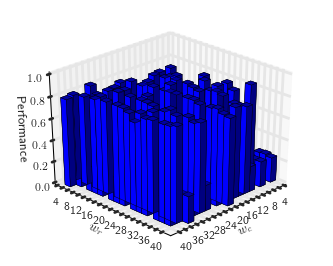
\includegraphics[width=1.0\columnwidth]{img/motivation_1}
\vspace{-1.5em} % Shrink vertical padding
\caption{}
\label{fig:motivation-1}
\end{subfigure}
~%
\begin{subfigure}[h]{.45\columnwidth}
\centering
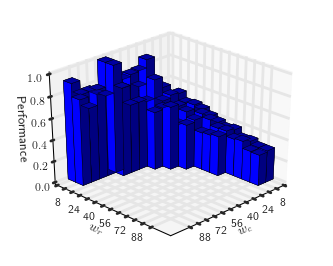
\includegraphics[width=1.0\columnwidth]{img/motivation_2}
\vspace{-1.5em} % Shrink vertical padding
\caption{}
\label{fig:motivation-2}
\end{subfigure}
\caption[Workgroup size optimisation space across devices]{%
  Workgroup size optimisation space of a stencil benchmark across
  devices: (\subref{fig:motivation-1}) Intel CPU,
  (\subref{fig:motivation-2}) NVIDIA GPU. This shows that stencil
  performance is dependent on properties of the underlying
  architecture, with different optimal workgroup sizes ($56 \times 20$
  vs.\ $64 \times 4$) for the two devices shown.%
}
\label{fig:motivation-arch}
\end{figure}

\begin{figure}
\centering
\begin{subfigure}[h]{.45\columnwidth}
\centering
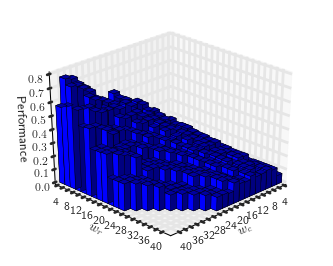
\includegraphics[width=1.0\columnwidth]{img/motivation_3}
\vspace{-1.5em} % Shrink vertical padding
\caption{}
\label{fig:motivation-3}
\end{subfigure}
~%
\begin{subfigure}[h]{.45\columnwidth}
\centering
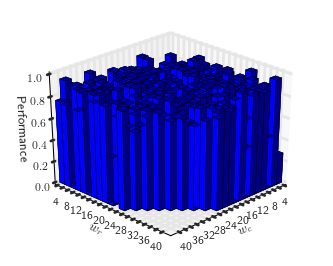
\includegraphics[width=1.0\columnwidth]{img/motivation_4}
\vspace{-1.5em} % Shrink vertical padding
\caption{}
\label{fig:motivation-4}
\end{subfigure}
\caption[Workgroup size optimisation space across stencils]{%
  Workgroup size optimisation space of two stencils on the same
  device. Despite the underlying hardware being the same, the relative
  performance of workgroup sizes varies greatly between the two
  programs. The optimal workgroup sizes are $128\times2$ and
  $256\times4$ respectively.%
}
\label{fig:motivation-prog}
\end{figure}

In this section I present the case for autotuning the workgroup size
of SkelCL stencil skeletons. Stencil workgroup sizes presents a two
dimensional parameter space, consisting of a number of rows and
columns. It is constrained by properties of both the stencil code and
underlying architecture. For a detailed discussion of the parameter
space and experimental methodology, see Sections~\ref{sec:background}
and~\ref{sec:methodology}.

By comparing the mean runtime of a stencil program using different
workgroup sizes while keeping all other conditions constant, we can
assess the relative performance of different points in the
optimisation space. Plotting this two dimensional optimisation space
using a three dimensional bar chart provides a quick visual overview
of the optimisation space. The two horizontal axes are used to
represent the number of rows and columns in a workgroup, while the
height of each bar shows the performance of a program at that point in
the space (higher is better).

If the performance of workgroup sizes were not dependent on the
execution device, we would expect the relative performance of points
in the optimisation space to be consistent across devices. As shown in
Figure~\ref{fig:motivation-arch}, this is not the case, with the
optimisation space of the same benchmark on different devices being
radically different. Not only does the optimal workgroup size change
between devices, but the performance of suboptimal workgroup sizes is
equally dissimilar.

The optimisation space of~\ref{fig:motivation-1} has a grid-like
structure, with clear performance advantages of workgroup sizes at
multiples of 8 columns. A developer specifically targeting this device
would learn to select workgroup sizes which follow this pattern. This
domain specific knowledge does not transfer to the device shown
in~\ref{fig:motivation-2}, where the relatively simple optimisation
space is more amenable to a stochastic hill climbing search.

Similarly, the optimisation space of two different stencils on the
same device is shown in~\ref{fig:motivation-prog}, demonstrating that
the optimisation space is dependent on the program being executed.

The optimal workgroup size is different for each of the four examples,
and the difference between the maximum and minimum performance
workgroup sizes provides an average $37.0\times$ speedup. The existing
SkelCL stencil implementation uses a statically chosen workgroup size
of $32\times4$, and this provides an average of only 63\% of the
available performance when compared to the best workgroup size for
these four examples. Even for this small set of examples, static
values and simple heuristics cannot provide portable performance. The
workgroup size parameter is sensitive to factors outside the influence
of the developers control, such as the type of program, the data being
operated on, and the execution device. This makes portable performance
tuning a difficult task, and it has traditionally been the
responsibility to domain specialists to laboriously hand tune
individual programs to match the target problem and underlying
hardware.

Given the important role that stencil codes play in many fields of
computer science and simulation, and the difficulties in selecting
workgroup sizes for portable performance, I believe that there is a
compelling case for the development of an autotuner which can
accommodate for these differences of workgroup size performance
between devices and programs. It is my hypothesis that the performance
of algorithmic skeletons will be improved by developing an autotuner
which considers dynamic features which cannot be determined at compile
time. The premise is that the optimisation spaces of algorithmic
skeletons such as stencils are shaped by features which can only be
determined at runtime. Effective searching of these spaces can only be
performed by collecting empirical data rather than building predictive
models.

The ambition of this thesis is to demonstrate that, using machine
learning, we can develop predictive tuning systems which closely
approach --- and in some cases, outperform --- the kinds of ad-hoc
hand tuning which traditionally came at the cost of many man hours of
work from expert programmers to develop.


\subsection{Structure}

The remainder of the document is structured as follows:
%
\begin{itemize}
\item Section~\ref{sec:background} contains necessary background
  material, an introduction to the SkelCL framework, and a description
  of the techniques used throughout the thesis;
\item Section~\ref{sec:related} contains an exposition of relevant
  literature in the field of autotuning and heterogeneous parallelism,
  contrasting the related research with my own;
\item % Section~\ref{sec:autotune} presents OmniTune, an extensible and
%   distributed autotuner capable of predicting optimisation parameter
%   values for unseen programs and devices at runtime;
% \item Section~\ref{sec:omnitune-skelcl} describes the application of
%   OmniTune for selecting the workgroup size of SkelCL stencils;
% \item Section~\ref{sec:methodology} describes a comprehensive
%   exploration of the workgroup size optimisation space for stencil
%   skeletons, including the methodology for obtaining performance data
%   and experimental setup;
% \item Section~\ref{sec:evaluation} evaluates the effectiveness of
%   OmniTune with respect to its accuracy, performance compared to human
%   experts, and a cost benefit analysis of autotuning;
\item Section~\ref{sec:conclusions} contains concluding remarks and
  plans for future work.
\end{itemize}


\subsection{Summary}

This introductory section has outlined the need for higher levels of
abstraction for parallel programming and the difficulty that this
provides for performance tuning. It advocates the use of adaptive
tuning for algorithmic skeletons, and describes the contributions of
this thesis towards this goal. In the next section, I provide an
overview of the techniques and methodology used in this thesis.


\section{Background}\label{sec:background}

This section provides a detailed though non-exhaustive description of
the theory and techniques used in this thesis. First is an overview of
algorithmic skeletons, GPGPU programming, and the combination of the
two in SkelCL. Second is an overview of the machine learning
techniques used in this thesis, followed by a description of the
Statistical tools tools and methodologies used in the evaluation.


\subsection{Algorithmic Skeletons}

Introduced by \citeauthor{Cole1989} in \citeyear{Cole1989},
algorithmic skeletons simplify the task of parallel programming by
abstracting common patterns of communication, providing parallel
implementations of higher order functions~\cite{Cole1989}. The
interfaces to generic parallel algorithms exposed by algorithmic
skeletons are parameterised by the user with \emph{muscle functions}
that implement problem specific logic. The idea is that this allows
the user to focus on solving the problem at hand, affording greater
ease of use by automating the coordination of parallel resources.


\subsubsection{Abstracting Task and Data Parallelism}

Algorithmic skeletons are categorised as either \emph{data} parallel
or \emph{task} parallel. In data parallel skeletons, data are
distributed across nodes for parallel processing, where each parallel
node executes the same code on a unique subset of the data. Examples
of data parallel algorithmic skeletons include \emph{map}, \emph{zip},
and \emph{reduce}. The data parallel operations provided by SkelCL are
described in detail in Subsection~\ref{subsec:skelcl-intro}.

Task parallel skeletons treat the data as a singular object and
instead parallelise the execution of multiple tasks. Tasks are
assigned to threads, which can communicate with each other by passing
data between threads. Examples of task parallel algorithmic skeletons
include \emph{pipe}, \emph{task farm}, and \emph{for loops}.


\subsubsection{Algorithmic Skeleton Frameworks}

\begin{figure}
\centering
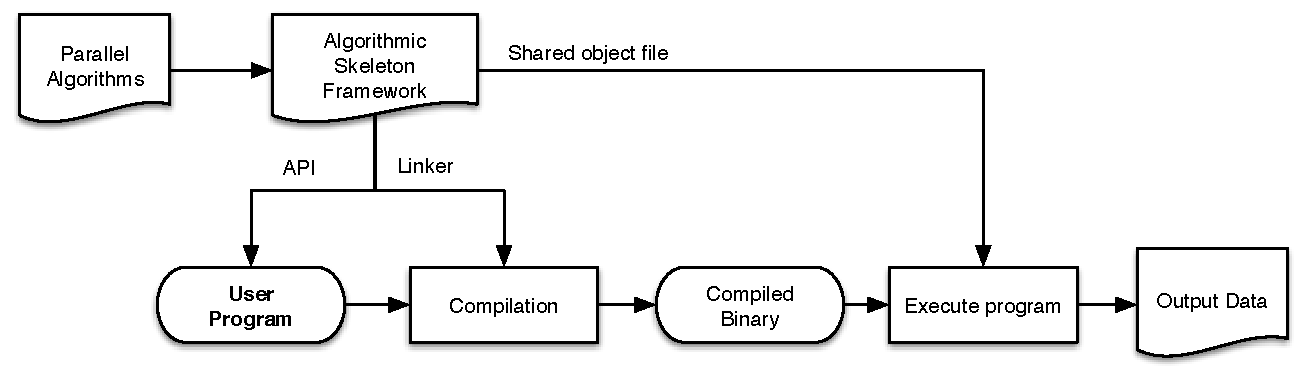
\includegraphics[width=0.99\columnwidth]{img/askf}
\caption[Overview of an Algorithmic Skeleton Framework]{%
  Typical usage of a library based Algorithmic Skeleton
  Framework. Other approaches to algorithmic skeletons involve
  embedding the API into the core language itself, or using template
  and macro substitution to remove the need for linking with a
  library.%
}
\label{fig:askf}
\end{figure}

Algorithmic Skeleton Frameworks (ASkFs) provide concrete parallel
implementations of parallel patterns, which are parameterised by the
user to generate specific problem solving programs. The interfaces
exposed by frameworks must be sufficiently generic to allow users to
express a range of problems.

Implementations of algorithmic skeletons abound, targeting a range of
different use cases and host languages. Notable examples include:
eSkel~\cite{Benoit2005a}, Skandium~\cite{Leyton2010}, and
FastFlow~\cite{Aldinucci2011}. The most prevalent form of ASkF is that
of the standalone library which exposes a set of public APIs, shown in
Figure~\ref{fig:askf}. See~\cite{Gonzalez2010} for a more exhaustive
review of ASkFs in the research literature.

In industry, Google's MapReduce~\cite{Dean2008} and Intel's Thread
Building Blocks~\cite{IntelTBB} have utilised a similar approach to
abstracting the coordination of parallel resources as in algorithmic
skeletons, to great commercial success, although they do not advertise
themselves as such.


\subsection{GPGPU Programming}\label{subsec:gpgpu}

General purpose programming with graphics hardware is a nascent field,
but has shown to enable massive data parallel throughput by
re-purposing the hardware traditionally dedicated to the rendering of
3D graphics for generic computation. This was enabled by hardware
support for programmable shaders replacing the fixed function graphics
pipeline, and support for floating point operations in
2001. \citeauthor{Owens2006} provide a review of the first five years
of general purpose computation on graphics hardware
in~\cite{Owens2006}.

In the ensuing progress towards increasingly programmable graphics
hardware, two dominant programming models have emerged: CUDA and
OpenCL, which both abstract the graphics primitives of GPU hardware
and provide a platform for GPGPU programming. CUDA is a language
developed by NVIDIA for programming their GPUs using a proprietary SDK
and API~\cite{Nvidia2007}, while OpenCL is a vendor-independent open
standard based on a subset of the ISO C99 programming language, with
implementations for devices from most major GPU
manufactures~\cite{Stone2010}. Quantitative evaluations of the
performance of CUDA and OpenCL programs suggest that performance is
comparable between the two systems, although the wider range of target
architectures for OpenCL means that appropriate optimisations must be
made by hand or by the compiler~\cite{Komatsu2010,Karimi2010}.


\subsubsection{The OpenCL Programming Model}

\begin{figure}
\centering
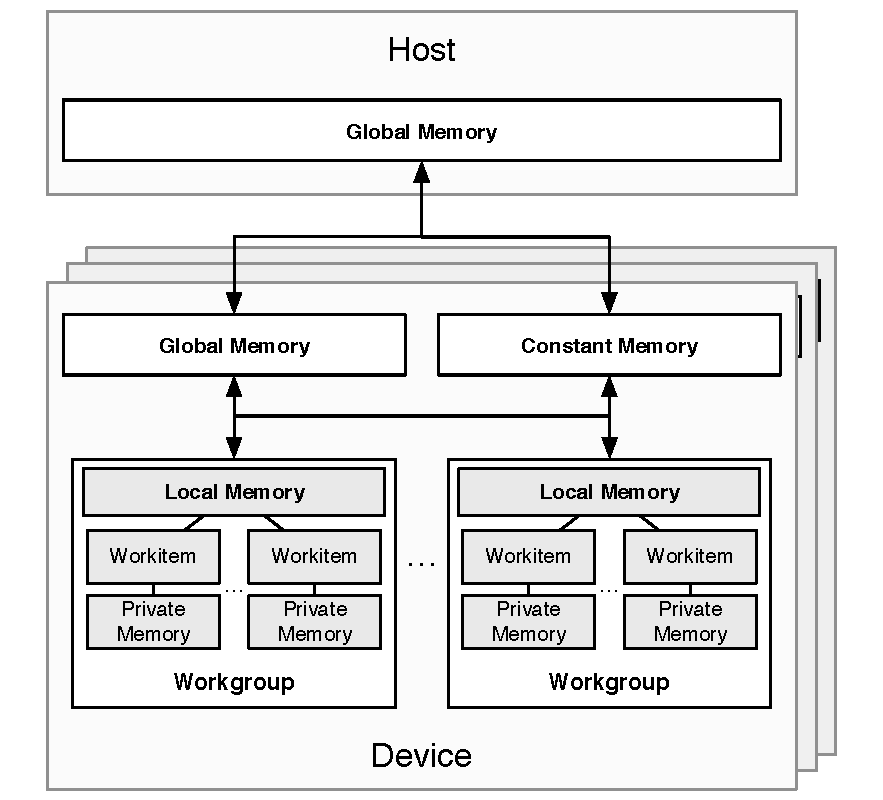
\includegraphics[width=.8\columnwidth]{img/opencl-memory}
\caption[The OpenCL memory model]{%
  The OpenCL memory model. The host communicates with each device
  through transfers between global memory spaces. The capacity of each
  type of memory is dependent on the device hardware. In general,
  private memory is the fastest and smallest, and global memory is the
  largest and slowest.%
}
\label{fig:opencl-memory}
\end{figure}

OpenCL is a parallel programming framework which targets CPUs, GPUs,
and other parallel processors such as Field-Programmable Gate
Arrays. It provides a set of APIs and a language (based on an extended
subset of C) for controlling heterogeneous \emph{compute devices} from
a central host. Programs written for these devices are called
\emph{kernels}, and are compiled by platform-specific tool chains. At
runtime, an OpenCL \emph{platform} is selected and a \emph{context}
object is created which exposes access to each supported compute
device through \emph{command queues}.  When a kernel is executed, each
unit of computation is referred to as a \emph{workitem}, and these
workitems are grouped into \emph{workgroups}. The sum of all workgroup
dimensions defines the \emph{global size}. For GPUs, workgroups
execute on the Single Instruction Multiple Data (SIMD) processing
units in lockstep. This is very different from the behaviour of
traditional CPUs, and can cause severe performance penalties in the
presence of flow control, as workitems must be stalled across divering
flow paths.


\paragraph{Memory Model}

Unlike the flat model of CPUs, OpenCL uses a hierarchical memory
model. The host and each OpenCL device has a single global memory
address space. Each workgroup has a local memory space, and each
workitem has a region of private memory.

Workgroups cannot access the memory of neighbouring workgroups, nor
can workitems access the private memory of other workitems. OpenCL
provides synchronisation barriers to allow for communication between
workitems within a single workgroup via the local memory, but not
global barriers. Memory transfers between the host and devices occurs
between global memory regions. In the case of programming
heterogeneous devices, these transfers must occur over the connection
bus between the CPU and device (e.g.\ PCIe for discrete GPUs), which
typically creates a performance bottleneck by introducing a
performance overhead to transfer data to the device for processing,
then back to the device afterwards. Direct transfers of data between
devices is not supported, requiring an intermediate transfer to the
host memory.


\paragraph{Performance Optimisations}

The wide range of supported execution devices and differing
standards-compliant implementations makes portable performance tuning
of OpenCL programs a difficult task~\cite{Rul2010}, and the
interactions between optimisations and the hardware are complex and
sometimes counter-intuitive~\cite{Ryoo2008}.

The overhead introduced by memory transfers between host and compute
devices further complicates comparisons of OpenCL performance on
different devices. The conclusion of~\cite{Gregg2011} is that this
overhead can account for a $2\times$ to $50\times$ difference of GPU
program runtime. In~\cite{Lee2010}, \citeauthor{Lee2010} present a
performance analysis of optimised throughput computing applications
for GPUs and CPUs. Of the 14 applications tested, they found GPU
performance to be $0.7\times$ to $14.9\times$ that of multi-threaded
CPU code, with an average of only 2.5$\times$. This is much lower than
the $100\times$ to $1000\times$ values reported by other studies, a
fact that they attribute to uneven comparison of optimised GPU code to
unoptimised CPU code, or vice versa. \citeauthor{Lee2010} found that
multithreading, cache blocking, reordering of memory accesses and use
of SIMD instructions to contribute most to CPU performance. For GPUs,
the most effective optimisations are reducing synchronization costs,
and exploiting local shared memory. In all cases, the programs were
optimised and hand-tuned by programmers with expert knowledge of the
target architectures. It is unclear whether their performance results
still hold for subsequent generations of devices.

Despite the concerns of over-represented speedups, the potential for
high performance coupled with the complexity and low levels of
abstraction provided by OpenCL make it an ideal target for skeletal
abstractions. SkelCL and SkePU are two such examples which add a layer
of abstraction above OpenCL and CUDA respectively in order to simplify
GPGPU programming~\cite{Enmyren2010}.

\subsection{High-Level GPU Programming with
  SkelCL}\label{subsec:skelcl-intro}

Introduced in~\cite{Steuwer2011}, SkelCL is an object oriented C++
library that provides OpenCL implementations of data parallel
algorithmic skeletons for heterogeneous parallelism using CPUs or
multi-GPUs. SkelCL addresses the parallel programmability challenge by
allowing users to easily harness the power of GPUs and CPUs for data
parallel computing.

The goal of SkelCL is to enable the transition towards higher-level
programming of GPUS, without requiring users to be intimately
knowledgeable of the concepts unique to OpenCL programming, such as
the memory or execution model~\cite{Steuwer2012}. SkelCL has been
shown to reduce programmer effort for developing real applications
through the use of robust pattern implementations and automated memory
management, maintaining performance within 5\% of that of equivalent
hand-written implementations in OpenCL~\cite{Steuwer2013}.

SkelCL skeletons are parameterised with muscle functions by the user,
which are compiled into OpenCL kernels for execution on device
hardware. SkelCL supports operations on one or two dimensional arrays
of data, with the Vector and Matrix container types transparently
handling lazy transfers between host and device memory, and supporting
partitioning for multi-GPU execution~\cite{Steuwer2013a}. SkelCL is
freely available and distributed under dual GPL and academic
licenses\footnote{\url{http://skelcl.uni-muenster.de}}.


\subsubsection{Pattern definitions}

SkelCL provides six skeletons for data parallel operations: $\map$,
$\zip$, $\reduce$, $\scan$, $\allpairs$, and $\stencil$. The focus of
this thesis is on tuning the $\stencil$ skeleton, but for the sake of
completeness I provide here a brief overview of the behaviour of all
six patterns.


\paragraph{Map}

The $\map$ operation is a basic building block of data parallel
algorithms. Given a customising function $f$ and a vector $x$ of $n$
elements, the $\map$ operation applies the function $f$ to each
element $x_1, x_2, \ldots, x_n$, returning a vector of the same
length:
%
\begin{equation}
\map\left(f, [x_1,x_2,\ldots,x_n]\right) \to [f(x_1),f(x_2),\ldots,f(x_n)]
\end{equation}
%
The process is the same for an $n \times m$ matrix:
%
\begin{equation}
\begin{split}
\map\left(f,
\begin{bmatrix}
  x_{11} & \cdots & x_{1m} \\
  \vdots & \ddots & \vdots \\
  x_{n1} & \cdots & x_{nm}
\end{bmatrix}\right) \\
\to
\begin{bmatrix}
  f(x_{11}) & \cdots & f(x_{1m}) \\
  \vdots & \ddots & \vdots \\
  f(x_{n1}) & \cdots & f(x_{nm})
\end{bmatrix}
\end{split}
\end{equation}
%
Execution of the customising function can be parallelised as each
element is processed independently. There are no guarantees on
execution ordering.


\paragraph{Zip}

The $\zip$ operation combines elements of containers pairwise. Given a
binary operator $\oplus$ and two vectors $x$ and $y$ of $n$ elements
each:
%
\begin{equation}
\begin{split}
\zip\left( \oplus, [x_1,x_2,\ldots,x_n], [y_1,y_2,\ldots,y_n] \right) \\
\to
\left[ x_1 \oplus y_1, x_2 \oplus y_2, \ldots, x_n \oplus y_n \right]
\end{split}
\end{equation}
%
For two matrices of $n \times m$ elements each:
%
\begin{equation}
\begin{split}
\zip \left( \oplus,
\begin{bmatrix}
  x_{11} & \cdots & x_{1m} \\
  \vdots & \ddots & \vdots \\
  x_{n1} & \cdots & x_{nm}
\end{bmatrix},
\begin{bmatrix}
  y_{11} & \cdots & y_{1m} \\
  \vdots & \ddots & \vdots \\
  y_{n1} & \cdots & y_{nm}
\end{bmatrix} \right) \\
\to
\begin{bmatrix}
  x_{11} \oplus y_{11} & \cdots & x_{1m} \oplus y_{1m} \\
  \vdots & \ddots & \vdots \\
  x_{n1} \oplus y_{n1} & \cdots & x_{nm} \oplus y_{nm}
\end{bmatrix}
\end{split}
\end{equation}
%
The $\zip$ operation is parallelised in the same manner as $\map$.


\paragraph{Reduce}

The $\reduce$ operator combines all elements of an input vector and
returns a scalar. Given a binary operator $\oplus$, its identity
$\bm{i}$ and a vector $x$ of $n$ elements:
%
\begin{equation}
\begin{split}
  \reduce \left( \oplus, \bm{i}, [x_1,x_2,\ldots,x_n] \right) \\
  \to
  x_1 \oplus x_2 \oplus \ldots \oplus x_n
\end{split}
\end{equation}
%
For a $n \times m$ matrix:
%
\begin{equation}
\begin{split}
\reduce \left( \oplus, i,
\begin{bmatrix}
  x_{11} & \cdots & x_{1m} \\
  \vdots & \ddots & \vdots \\
  x_{n1} & \cdots & x_{nm}
\end{bmatrix} \right) \\
\to
x_{11} \oplus x_{12} \oplus \ldots \oplus x_{nm}
\end{split}
\end{equation}
%
Reduction operates by recursively combining elements, storing
intermediate results in fast local memory. No guarantee is made on
execution ordering, so the binary operator must be associative.


\paragraph{Scan}

The $\scan$ operator applies a binary function $\oplus$ to each member
of an input array $x$ of $n$ elements, such that element $x_i$ at the
$i$th position is calculated by applying the binary function to all
elements $x_1,x_2, \ldots x_{i-1}$. For the first element $x_i$, the
value is the identify $\bm{i}$ of the $\oplus$ operator:
%
\begin{equation}
\begin{split}
  \scan \left( \oplus, \bm{i}, [x_1,x_2,\ldots,x_n] \right) \\
  \to
  \left[ \bm{i}, x_1, x_1 \oplus x_2, \ldots, x_1 \oplus x_2 \oplus
    \ldots \oplus x_n \right]
\end{split}
\end{equation}
%
The SkelCL scan implementation is heavily optimised to make use of
local memory, based on the design from~\cite{Harris2007a}.


\paragraph{AllPairs}

The AllPairs skeleton is a specialised pattern for Matrix Matrix
operations, introduced in~\cite{Steuwer2014}. Given two matrices of
size $n \times d$ and $n \times m$, a binary operator $\oplus$:
%
\begin{equation}
\begin{split}
\allpairs \left( \oplus,
\begin{bmatrix}
  x_{11} & \cdots & x_{1d} \\
  \vdots & \ddots & \vdots \\
  x_{n1} & \cdots & x_{nd}
\end{bmatrix},
\begin{bmatrix}
  y_{11} & \cdots & y_{1m} \\
  \vdots & \ddots & \vdots \\
  y_{n1} & \cdots & y_{nm}
\end{bmatrix} \right) \\
\to
\begin{bmatrix}
  z_{11} & \cdots & z_{1m} \\
  \vdots & \ddots & \vdots \\
  z_{n1} & \cdots & z_{nm}
\end{bmatrix}
\end{split}
\end{equation}
%
where:
%
\begin{equation}
z_{ij} =
\left[ x_{i1}, x_{i2}, \ldots, x_{id} \right] \oplus
\left[ y_{j1}, y_{j2}, \ldots, y_{jd} \right]
\end{equation}
%
An additional implementation is provided for when the $\oplus$
operator is known to match that of a zip pattern:
%
\begin{equation}
z_{ij} =
\left[
  x_{i1}, \oplus y_{j1}, x_{i2} \oplus y_{j2}, \ldots, x_{id} \oplus y_{jd}
\right]
\end{equation}
%
This pattern has applications from bioinformatics to matrix
multiplication, and uses fast local memory to reduce data access times
for repeated reads.


\paragraph{Stencil}

\begin{figure}
\centering
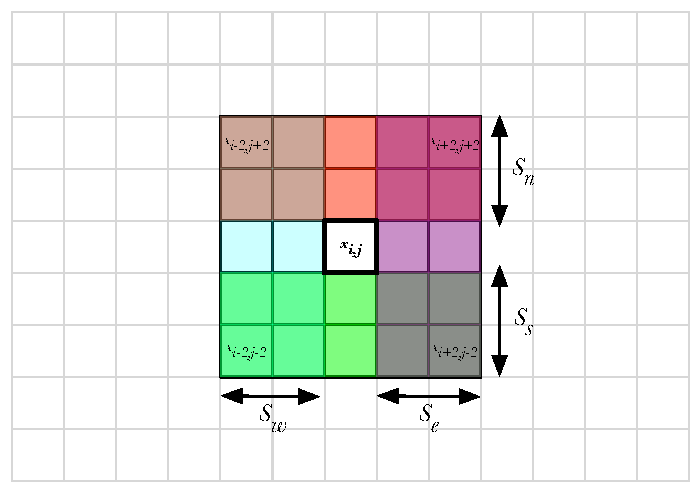
\includegraphics[width=.6\columnwidth]{img/stencil-shape}
\caption[Stencil border region]{%
  The border region of a stencil is defined using a stencil shape $S$,
  consisting of the four independent components describing the number
  of cells north $S_n$, east $S_e$, west $S_w$, and south $S_s$.%
}
\label{fig:stencil-shape}
\end{figure}

Stencils are patterns of computation which operate on uniform grids of
data, where the value of each cell is updated based on its current
value and the value of one or more neighbouring elements, called the
\emph{border region}. Introduced in~\cite{Breuer2014}, SkelCL provides
a 2D stencil skeleton which allows users to provide a function which
updates a cell's value, while SkelCL orchestrates the parallel
execution of this function across all cells.

The border region is described by a \emph{stencil shape}, which
defines an $i \times j$ rectangular region about each cell which is
used to update the cell value. Stencil shapes may be asymmetrical, and
are defined in terms of the number of cells in the border region to
the north, east, south, and west of each cell, shown in
Figure~\ref{fig:stencil-shape}. Given a customising function $f$, a
stencil shape $S$, and an $n \times m$ matrix:
%
\begin{equation}
\begin{split}
\stencil \left( f, S,
\begin{bmatrix}
  x_{11} & \cdots & x_{1m} \\
  \vdots & \ddots & \vdots \\
  x_{n1} & \cdots & x_{nm}
\end{bmatrix} \right) \\
\to
\begin{bmatrix}
  z_{11} & \cdots & z_{1m} \\
  \vdots & \ddots & \vdots \\
  z_{n1} & \cdots & z_{nm}
\end{bmatrix}
\end{split}
\end{equation}
%
where:
%
\begin{equation}
z_{ij} = f \left(
\begin{bmatrix}
  z_{i-S_n,j-S_w} & \cdots & z_{i-S_n,j+S_e} \\
  \vdots & \ddots & \vdots \\
  z_{i+S_s,j-S_w} & \cdots & z_{i+S_s,j+S_e}
\end{bmatrix} \right)
\end{equation}
%
Note that a stencil operation in which the size of the stencil shape
$S$ is zero in every direction is functionally equivalent to a $\map$
operation. Where the border region includes elements outside of the
matrix, values are substituted from either a predefined padding value,
or the value of the nearest cell within the matrix, depending on user
preference.

A popular usage of Stencil codes is for solving problems iteratively,
whereby a stencil operation is repeated over a range of discrete time
steps $0 \le t \le t_{max}$, and $t \in \mathbb{Z}$. An iterative
stencil operation $g$ accepts a customising function $f$, a Stencil
shape $S$, and a matrix $M$ with initial values $M_{init}$. The value
of an iterative stencil can be defined recursively as:
%
\begin{equation}
g(f, S, M, t) =
\begin{cases}
  \stencil \left( f, S, g(f, S, M, t-1) \right),& \text{if } t \geq 1\\
  M_{init}, & \text{otherwise}
\end{cases}
\end{equation}
%
Examples of iterative stencils are cellular automata. Another
extension of the stencil operation accepts an ordered list of
customising functions which are applied sequentially for each
iteration. This has applications for multi-stage stencil operations
such as Canny Edge Detection, in which four distinct stencil
operations are performed as a sequence.


\subsubsection{Implementation Details}

Each skeleton is represented by a template class, declared in a header
file detailing the public API, e.g.\ \path{SkelCL/Stencil.h}. A
private header file contains the template class declaration, e.g.\
\path{SkelCL/detail/StencilDef.h}. Small OpenCL kernels are stored as
inline strings inside the definition headers. Non-trivial OpenCL
kernels are stored in separate source files, e.g.\
\path{SkelCL/detail/StencilKernel.cl}. Muscle functions are passed as
OpenCL strings to the skeleton template classes, and the LLVM API is
used to perform argument and function name substitution.

\paragraph{Stencil Implementation}

For the stencil skeleton, each cell maps to a single work item; and
this collection of work items is then divided into \emph{workgroups}
for execution on the target hardware. In a stencil code, each
work-item reads the value of the corresponding grid elements, and the
surrounding elements defined by the border region. Since the border
regions of neighbouring elements overlap, the value of all elements
within a workgroup are stored in a \emph{tile}, which is a region of
local memory. As local memory access times are much smaller than that
of global memory, this greatly reduces the latency of the border
region reads performed by each workitem. Changing the workgroup size
thus affects the amount of local memory required for each workgroup,
which in turn affects the number of workgroups which may be
simultaneously active. So while the user defines the size, type, and
border region of the of the grid being operated upon, it is the
responsibility of the SkelCL stencil implementation to select an
appropriate workgroup size to use.

\begin{figure}
\centering
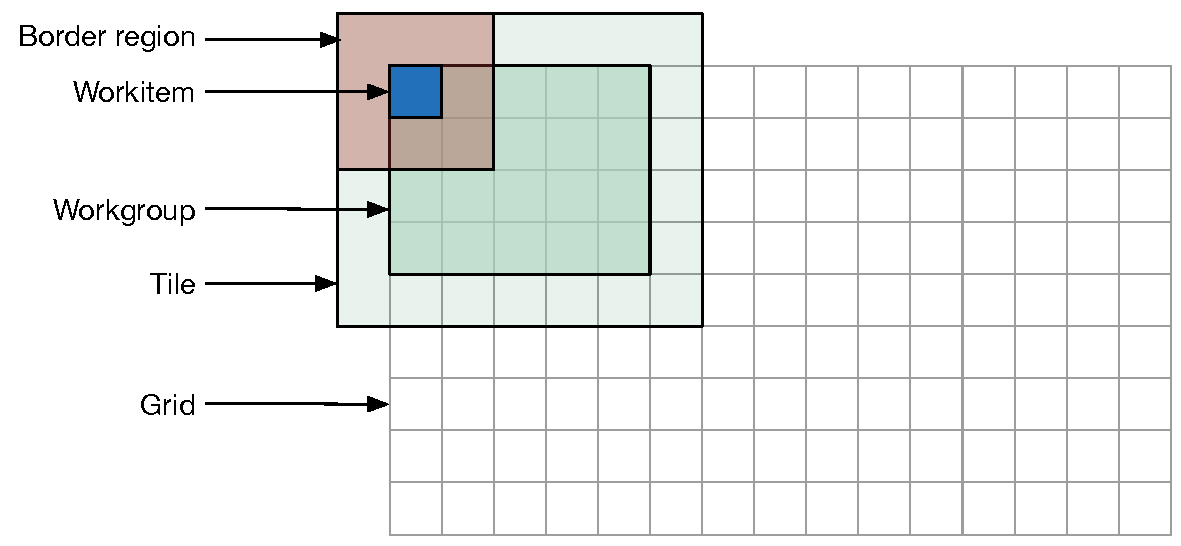
\includegraphics[width=.75\columnwidth]{img/stencil-wg}
\caption[Workgroup decomposition in stencils]{%
  The components of a stencil: a grid of cells is decomposed into
  workgroups, consisting of multiple workitems. Each work item
  operates on a border region, and the size of the workgroup and outer
  border region defines a tile, which is a region of local memory
  allocated to each workgroup.%
}
\label{fig:stencil-wg}
\end{figure}


\subsection{Machine Learning}


Multiple machine learning methods are used in this thesis to perform
classification and regression tasks. Classification is the task of
predicting the correct category --- or class --- for a new instance,
based on ``labelled'' training data, i.e.\ instances whose categories
are known. The properties describing instances are called
\emph{features}. The purpose of regression is to predict the
relationship between a dependent variable and the value of one or more
independent variables. Unlike with classification, the predicted
dependent variable can be continuous, rather than categorical. This
subsection briefly describes the properties of classifiers and regressors
used in this thesis.


\paragraph{ZeroR}

A ``ZeroR'' classifier represents the simplest approach to
classification, in that it ignores all features, and simply predicts
the mode of the training data labels. This is useful for providing a
baseline to evaluate the performance of more complex classifiers
against, since a ZeroR classifier has no power of prediction.


\paragraph{Naive Bayes}

Naive Bayes classifiers are probabilistic classifiers which assume
strong independence between features. That is, the value of one
feature is considered independently of another, and is what lends the
\emph{Naive} portion of the name. The goal of Naive Bayes is to
predict the probability of a class $y$, given a set of $d$ independent
variables $x = x_1, x_2, \ldots x_d$. Naive Bayes applies Bayes
theorem, which states that given a \emph{prior} (i.e.\ unconditional)
probability for each class $P(y)$, a class-\emph{conditional} model
$P(x|y)$, and a normaliser across all classes
$P(x) = \sum_{y'}P(x|y')P(y')$: the probability of a class $y$ given
dependent variables $x$ is equal to the probability of $x$ given $y$,
multiplied by the probability of $y$:
%
\begin{equation}
  P(y|x) = \frac{P(x|y)P(y)}{\sum_{y'}P(x|y')P(y')}
\end{equation}
%
The class which has the highest probability from the set of possible
classes $Y$ is the prediction. Note that the normaliser $P(x)$ does
not affect the class which is most likely. The class conditional model
uses ``counts'' for each observation based on training data:
%
\begin{equation}
  P(x|y) = \prod_{i=1}^{d} P(x_i|y)
\end{equation}
%
The simplicity of Naive Bayes makes it attractive for various purposes
such as text classification (using word frequency as features), but
the assumption of independence makes it unsuitable for certain use
cases.


\paragraph{Decision Trees}

Decision trees are an intuitive form of classification in which a tree
structure of decision nodes are used to predict the class for a given
set of features. Decision trees are built using binary recursive
partitioning: by creating a decision node for the feature which
provides the highest gain, creating new child nodes for each possible
outcome, splitting dividing the data amongst these child nodes, and
recursing. To find the gain of an feature, we first compute the
entropy of the data set. Given a set of data points $D$, and $p_{(+)}$
and $p_{(-)}$ are the number of positive and negative examples in $D$:
%
\begin{equation}
  H(D) = - p_{(+)}\log_2p_{(+)} - p_{(-)}\log_2p_{(-)}
\end{equation}
%
The gain of an feature $x$ is then found using:
%
\begin{equation}
  \gain(D, x) = H(D) - \sum_{V \in \text{Values}(x)}\frac{|D_V|}{|D|}H(D_V)
\end{equation}
%
Decision trees are very popular and low overhead form of
classification, as they can be implemented using a nested set of
\texttt{if}/\texttt{else} statements. However, they can often overfit
to the training data.


\paragraph{Random Forest}

Random Forests are an ensemble technique which attempt to overcome the
tendency of decision trees to overfit to training data by training
multiple decision trees and using the mode of each tree to select
predictions~\cite{Breiman1999}. Alternatively they can be trained
using regression trees, in which case the predicted value is the mean
output of all trees.


% \paragraph{Logistic Regression}

% A logistic regressor is a set of linear weights and a bias fitted with
% a logistic squashing function in order to generate a sigmoid shape
% decision boundary.


% \paragraph{SMO}


\subsection{Statistics}

This subsection describes a number of the statistical tools used
throughout this thesis.

% \paragraph{Statistical Testing}

% Student's \emph{t}-test


\paragraph{Interquartile Range}

For a given set of ordered data values, the quartiles are the three
points that divide the data set into four groups of equal size. The
first quartile is the point which $Q_1$ divides the data equally
between the lowest value and the median, $Q_2$. The third quartile
$Q_3$ is the point which divides the data between the median and the
highest value. The interquartile range (IQR) measures the dispersion
of a data set, and is the difference between the third and first
quartiles, $Q_3 - Q_1$.


\paragraph{Confidence Intervals}

Confidence intervals estimate the interval for the true range of a
population parameter. Given a set of samples of a population with
estimates of a parameter value for each, the confidence interval
$(c_1,c_2)$ estimates the frequency that the true parameter value will
fall between the per-sample confidence interval. Given a sample $x$
with sample size $n$, the confidence interval for a confidence
$\alpha$ is found using:
%
\begin{align}
  \bar{x} &= \frac{1}{n}\sum_{i=1}^{n} x_i\\
  \sigma &= \sqrt{\frac{\sum_{i=1}^{n}(x_i - \bar{x})^2}{n - 1}}\\
  c_1 &= \bar{x} - z_{1-\alpha/2}\frac{\sigma}{\sqrt{n}}\\
  c_2 &= \bar{x} + z_{1-\alpha/2}\frac{\sigma}{\sqrt{n}}
\end{align}
%
Where the value $z_{1-\alpha/2}$ assumes a Gaussian distribution of
the underlying data, and the values for popular $\alpha$ values are
typically found using pre-computed ``Z-tables''. To calculate
confidence intervals for the ratio of two means, $\bar{x}_1$ and
$\bar{x}_2$ with sample sizes $n_1$ and $n_2$, and respective standard
deviations $\sigma_1$ and $\sigma_2$:
%
\begin{align}
  \sigma_x &= \sqrt{\frac{\sigma_1^2}{n_1} + \frac{\sigma_2^2}{n_2}}\\
  c_1 &= \bar{x}_1 - \bar{x}_2 - z_{1-\alpha/2}\sigma_x\\
  c_2 &= \bar{x}_1 - \bar{x}_2 + z_{1-\alpha/2}\sigma_x
\end{align}
%
The above calculations assumes that the sample variance ($\sigma^2$)
is an accurate estimation of the true population variance. This relies
on the assumption of an underlying Gaussian distribution, which,
according to the central limit theorem, is true of large sample sizes
(typically $n \ge 30$).  In cases of smaller sample sizes, the sample
and population variances can differ significantly, so one must instead
use a Student's $t$-distribution, $t_{1-\alpha/2}$, in place of
$z_{1-\alpha/2}$.


\paragraph{Histogram}

Histograms are a widely used statistical visualisation which shows the
distribution of numerical data. The data is first divided into a set
of discrete, equally sized sub-intervals, or \emph{bins}. The number
of data points in each bin is used to show visualise the density
distribution. The shortcoming of histograms is that their appearance
is heavily influenced by three user-selected parameters: the number of
bins, the width of bins (binwidth), and the endpoints chosen. As such,
they may provide a misleading representation of the data if
inappropriate values for any of these parameters are chosen. Kernel
Density estimation is a technique for showing the distribution of data
which circumvents some of these issues.


\paragraph{Kernel Density Estimation}

A Kernel Density Estimate (KDE) is an approximation of the probability
density function of a random variable. Given a random variable $x$,
and bandwidth $h$ and a kernel $K$, the Kernel Density Estimate
$\hat{f}_h(x)$ can be found using:
%
\begin{equation}
  \hat{f}_h(x) = \frac{1}{nh} \sum^{n}_{i=1} K\left( \frac{x - x_i}{h} \right)
\end{equation}
%
Using a smooth kernel such as a Gaussian distribution for the kernel
produces a smooth density estimated, unlike histograms. However, like
histograms, the appearance of a Kernel Density Estimate plot is
dependent on the value of the bandwidth parameter $h$ (equivalent to
binwidth in histograms), so care must be taken to select a value to
minimise over or under smoothing. Grouped data can be shown by
plotting multiple KDEs on the same axes, although if the number of
groups is large, a box plot or violin plot may be more appropriate.


\paragraph{Box plot}

Box plots are used to show the distribution of quartile ranges for
grouped data. The contain the following features:
%
\begin{itemize}
\item Horizontal lines at the lower quartile, median and upper
  quartile.
\item Vertical lines above and below the upper and lower quartiles to
  the most extreme data point within 1.5 IQR of the upper/lower
  quartile, with horizontal whiskers at the end of the vertical lines.
\item Dots beyond the ends of the vertical lines to show outliers.
\end{itemize}
%
A variation of box plots used in this thesis is the violin plot, which
extends the box plot with a fitted Kernel Density Estimate plot to
show the probability \emph{density} of data at different values. To
construct a violin plot, KDEs for each group are rotated and mirrored
to generate a smoothed visualisation of the distribution.


\subsection{Summary}

This section gave a brief introduction to general-purpose computing
using graphics hardware, the OpenCL framework, and SkelCL. It was
followed by a description of the machine learning techniques used
throughout this thesis, and the statistical tools used for the
evaluation. In the next section, I review the state of the art in the
field of autotuning, and provide context for the contributions of this
thesis.


\section{Related Work}\label{sec:related}

This section begins with a brief survey of the broad field of
literature that is relevant to algorithmic skeletons. This is followed
by a review of the current state of the art in autotuning research,
focusing on heterogeneous parallelism, algorithmic skeletons, and
stencil codes. It presents the context and rationale for the research
undertaken for this thesis.


\subsection{Automating Parallelism}

It is widely accepted that parallel programming is difficult, and the
continued repetition of this claim has become something of a trite
mantra for the parallelism research community. An interesting
digression is to discuss some of the ways in which researchers have
attempted to tackle this difficult problem, and why, despite years of
research, it remains an ongoing challenge.

The most ambitious and perhaps daring field of parallelism research is
that of automatic parallelisation, where the goal is to develop
methods and systems to transform arbitrary sequential code into
parallelised code. This is a well studied subject, with the typical
approach being to perform these code transformations at the
compilation stage. In \citeauthor{Banerjee1993}'s thorough
review~\cite{Banerjee1993} on the subject, they outline the key
challenges of automatic parallelisation:
%
\begin{itemize}
\item determining whether sequential code can be legally transformed
  for parallel execution; and
\item identifying the transformation which will provide the highest
  performance improvement for a given piece of code.
\end{itemize}
%
Both of these challenges are extremely hard to tackle. For the former,
the difficulties lie in performing accurate analysis of code
behaviour. Obtaining accurate dynamic dependency analysis at compile
time is an unsolved problem, as is resolving pointers and points-to
analysis~\cite{Atkin-granville2013, Hind2001,Ghiya2001}.

The result of these challenges is that reliably performant, automatic
parallelisation of arbitrary programs remains a far from reached goal;
however, there are many note worthy variations on the theme which have
been able to achieve some measure of success.

One such example is speculative parallelism, which circumvents the
issue of having incomplete dependency information by speculatively
executing code regions in parallel while performing dependency tests
at runtime, with the possibility to fall back to ``safe'' sequential
execution if correctness guarantees are not
met~\cite{Prabhu2010,Trachsel2010}.  In~\cite{Jimborean2014},
\citeauthor{Jimborean2014} present a system which combines polyhedral
transformations of user code with binary algorithmic skeleton
implementations for speculative parallelisation, reporting speedups
over sequential code of up to $15.62\times$ on a 24 core processor.

Another example is PetaBricks, which is a language and compiler
enabling parallelism through ``algorithmic choice''~\cite{Ansel2009,
  Ansel2010}. With PetaBricks, users provide multiple implementations
of algorithms, optimised for different parameters or use cases. This
creates a search space of possible execution paths for a given
program. This has been combined with autotuning techniques for
enabling optimised multigrid programs~\cite{Chan2009}, with the wider
ambition that these autotuning techniques may be applied to all
algorithmic choice programs~\cite{Ansel2014}. While this helps produce
efficient parallel programs, it places a great burden on the
developer, requiring them to provide enough contrasting
implementations to make a search of the optimisation space fruitful.

Annotation-driven parallelism takes a similar approach. The user
annotates their code to provide ``hints'' to the compiler, which can
then perform parallelising transformations. A popular example of this
is OpenMP, which uses compiler pragmas to mark code sections for
parallel or vectorised execution~\cite{Dagum1998}. Previous work has
demonstrated code generators for translating OpenMP to
OpenCL~\cite{Grewe2013} and CUDA~\cite{Lee2009}. Again,
annotation-driven parallelism suffers from placing a burden on the
developer to identify the potential areas for parallelism, and lacks
the structure that algorithmic skeletons provide.

Algorithmic skeletons contrast the goals of automatic parallelisation
by removing the challenge of identifying potential parallelism from
compilers or users, instead allowing users to frame their problems in
terms of well defined patterns of computation. This places the
responsibility of providing performant, well tuned implementations for
these patterns on the skeleton author.


\subsection{Iterative Compilation \& Machine
  Learning}\label{subsec:iterative-compilation}

Iterative compilation is the method of performance tuning in which a
program is compiled and profiled using multiple different
configurations of optimisations in order to find the configuration
which maximises performance. One of the the first formalised
publications of the technique appeared in \citeyear{Bodin1998} by
\citeauthor{Bodin1998}~\cite{Bodin1998}.  Iterative compilation has
since been demonstrated to be a highly effective form of empirical
performance tuning for selecting compiler optimisations.

Given the huge number of possible compiler optimisations (there are
207 flags and parameters to control optimisations in GCC v4.9), it is
often unfeasible to perform an exhaustive search of the entire
optimisation space, leading to the development of methods for reducing
the cost of evaluating configurations. These methods reduce evaluation
costs either by shrinking the dimensionality or size of the
optimisation space, or by guiding a directed search to traverse a
subset of the space.

Machine learning has been successful applied to this problem,
in~\cite{Stephenson2003}, using ``meta optimisation'' to tune compiler
heuristics through an evolutionary algorithm to automate the search of
the optimisation space. \citeauthor{Fursin2011} continued this with
Milepost GCC, the first machine learning-enabled self-tuning
compiler~\cite{Fursin2011}. A recent survey of the use of machine
learning to improve heuristics quality by \citeauthor{Burke2013}
concludes that the automatic \emph{generation} of these self-tuning
heuristics but is an ongoing research challenge that offers the
greatest generalisation benefits~\cite{Burke2013}.

% An approach to online tuning of parallel programs is presented
% in~\cite{Ansel2012} which partitions the available parallel resources
% of a device in to two partitions and then executes two different
% configurations simultaneously using each partition. The configuration
% used for one of the configuration is guaranteed to be ``safe'', and
% the performance

% % Eastep, J., Wingate, D., & Agarwal, A. (2011). Smart Data
% % Structures: An Online Machine Learning Approach to Multicore Data
% % Structures. In Proceedings of the 8th ACM International Conference
% % on Autonomic Computing (pp. 11–20). New York, NY, USA:
% % ACM. doi:10.1145/1998582.1998587
% \TODO{Online reinforcement learning for optimising data structures
%   online, \cite{Tesauro2005}}

% % Tesauro, G. (2005). Online Resource Allocation Using Decompositional
% % Reinforcement Learning. In AAAI (pp. 886–891).
% \TODO{Reinforcement learning for resource allocation~\cite{Eastep2011}}

% % W. F. Ogilvie, P. Petoumenos, Z. Wang, and H. Leather, “Intelligent
% % Heuristic Construction with Active Learning,” in 18th International
% % Workshop on Compilers for Parallel Computing, 2015.
% \TODO{Using Active Learning to speed up the learning of compiler
%   heuristics~\cite{Ogilvie2015}. Towards online autotuning, albeit
%   only with binary optimisation parameter.}

%
% SOME EXAMPLES OF ML IN THE WILD:
%

% % R. Bitirgen, E. Ipek, and J. F. Martinez, “Coordinated Management of
% % Multiple Interacting Resources in Chip Multiprocessors: A Machine
% % Learning Approach,” in 2008 41st IEEE/ACM International Symposium on
% % Microarchitecture, 2008, pp. 318–329.
% \TODO{Artificial Neural Networks for resource allocation of CMPS:
% \cite{Bitirgen2008}}

% % Z. Wang and M. F. P. O. Boyle, “Partitioning Streaming Parallelism
% % for Multi-cores: A Machine Learning Based Approach,” in Proceedings
% % of the 19th international conference on Parallel architectures and
% % compilation techniques, 2010, pp. 307–318.
% \TODO{Offline ML for partitioning streaming applications:
% \cite{Wang2010}}

In~\cite{Saclay2010,Memon2013,Fursin2014}, \citeauthor{Fursin2014}
advocate a collaborative and ``big data'' driven approach to
autotuning, arguing that the challenges facing the widespread adoption
of autotuning and machine learning methodologies can be attributed to:
a lack of common, diverse benchmarks and datasets; a lack of common
experimental methodology; problems with continuously changing hardware
and software stacks; and the difficulty to validate techniques due to
a lack of sharing in publications. They propose a system for
addressing these concerns, the Collective Mind knowledge system,
which, while in early stages of ongoing development, is intended to
provide a modular infrastructure for sharing autotuning performance
data and related artifacts across the internet. In addition to sharing
performance data, the approach taken in this thesis emphasises the
collective \emph{exploitation} of such performance data, so that data
gathered from one device may be used to inform the autotuning
decisions of another. This requires each device to maintain local
caches of shared data to remove the network overhead that would be
present from querying a single centralised data store during execution
of a hot path. The current implementation of Collective Mind uses a
NoSQL JSON format for storing performance data. The relational schema
used in this thesis offers greater scaling performance and lower
storage overhead as the amount of performance data grows.

Whereas iterative compilation requires an expensive offline training
phase to search an optimisation space, dynamic optimisers perform this
optimisation space exploration at runtime, allowing programs to
respond to dynamic features ``online''. This is a challenging task, as
a random search of an optimisation space may result in configurations
with vastly suboptimal performance. In a real world system, evaluating
many suboptimal configurations will cause a significant slowdown of
the program. Thus a requirement of dynamic optimisers is that
convergence time towards optimal parameters is minimised.

Existing dynamic optimisation research has typically taken a low level
approach to performing optimisations. Dynamo is a dynamic optimiser
which performs binary level transformations of programs using
information gathered from runtime profiling and
tracing~\cite{Bala2000}. While this provides the ability to respond to
dynamic features, it restricts the range of optimisations that can be
applied to binary transformations. These low level transformations
cannot match the performance gains that higher level parameter tuning
produces.

An interesting related tangent to iterative compilation is the
development of so-called ``superoptimisers''. In~\cite{Massalin1987},
the smallest possible program which performs a specific function is
found through a brute force enumeration of the entire instruction
set. Starting with a program of a single instruction, the
superoptimiser tests to see if any possible instruction passes a set
of conformity tests. If not, the program length is increased by a
single instruction and the process repeats. The exponential growth in
the size of the search space is far too expensive for all but the
smallest of hot paths, typically less than 13 instructions. The
optimiser is limited to register to register memory transfers, with no
support for pointers, a limitation which is addressed
in~\cite{Joshi2002}. Denali is a superoptimiser which uses constraint
satisfaction and rewrite rules to generate programs which are
\emph{provably} optimal, instead of searching for the optimal
configuration through empirical testing. Denali first translates a low
level machine code into guarded multi-assignment form, then uses a
matching algorithm to build a graph of all of a set of logical axioms
which match parts of the graph, before using boolean satisfiability to
disprove the conjecture that a program cannot be written in $n$
instructions. If the conjecture cannot be disproved, the size of $n$
is increased and the process repeats.


\subsubsection{Training with Synthetic Benchmarks}

The use of synthetic benchmarks for providing empirical performance
evaluations dates back to as early as 1974~\cite{Curnow1976}. The
\emph{automatic generation} of such synthetic benchmarks is a more
recent innovation, serving the purpose initially of stress-testing
increasingly complex software systems for behaviour validation and
automatic bug detection~\cite{Verplaetse2000,Godefroid2008}. A range
of techniques have been developed for these purposes, ranging from
applying random mutations to a known dataset to generate test stimuli,
to so-called ``whitebox fuzz testing'' which analyses program traces
to explore the space of a program's control flow. Csmith is one such
tool which generates randomised C source programs for the purpose of
automatically detecting compiler bugs~\cite{Yang2012}.

A method for the automatic generation of synthetic benchmarks for the
purpose of \emph{performance} tuning is presented
in~\cite{Chiu2015}. \citeauthor{Chiu2015} use template substitution
over a user-defined range of values to generate training programs with
a statistically controlled range of features. A Perl preprocessor
generates output source codes from an input description using a custom
input language Genesis. Genesis is more flexible than the system
presented in this thesis, supporting substitution of arbitrary
sources. The authors describe an application of their tool for
generating OpenCL stencil kernels, but do not report any performance
results.


\subsection{Performance Tuning for Heterogeneous Parallelism}

As briefly discussed in Subsection~\ref{subsec:gpgpu}, the complex
interactions between optimisations and heterogeneous hardware makes
performance tuning for heterogeneous parallelism a difficult
task. Performant GPGPU programs require careful attention from the
developer to properly manage data layout in DRAM, caching, diverging
control flow, and thread communication. The performance of programs
depends heavily on fully utilising zero-overhead thread scheduling,
memory bandwidth, and thread grouping. \citeauthor{Ryoo2008a}
illustrate the importance of these factors by demonstrating speedups
of up to $432\times$ for matrix multiplication in CUDA by appropriate
use of tiling and loop unrolling~\cite{Ryoo2008a}. The importance of
proper exploitation of local shared memory and synchronisation costs
is explored in~\cite{Lee2010}.

In~\cite{Chen2014}, data locality optimisations are automated using a
description of the hardware and a memory-placement-agnostic
compiler. The authors demonstrate impressive speedups of up to
$2.08\times$, although at the cost of requiring accurate memory
hierarchy descriptor files for all targeted hardware. The descriptor
files must be hand generated, requiring expert knowledge of the
underlying hardware in order to properly exploit memory locality.

Data locality for nested parallel patterns is explored in~\cite{Lee}.
The authors use an automatic mapping strategy for nested parallel
skeletons on GPUs, which uses a custom intermediate representation and
a CUDA code generator, achieving $1.24\times$ speedup over hand
optimised code on 7 of 8 Rodinia benchmarks.

Reduction of the GPGPU optimisation space is demonstrated
in~\cite{Ryoo2008}, using the common subset of optimal configurations
across a set of training examples. This technique reduces the search
space by 98\%, although it does not guarantee that for a new program,
the reduced search space will include the optimal configuration.

\citeauthor{Magni2014} demonstrated that thread coarsening of OpenCL
kernels can lead to speedups in program performance between
$1.11\times$ and $1.33\times$ in~\cite{Magni2014}. The authors achieve
this using a machine learning model to predict optimal thread
coarsening factors based on the static features of kernels, and an
LLVM function pass to perform the required code transformations.

A framework for the automatic generation of OpenCL kernels from
high-level programming concepts is described in~\cite{Steuwer2015}. A
set of rewrite rules is used to transform high-level expressions to
OpenCL code, creating a space of possible implementations. This
approach is ideologically similar to that of PetaBricks, in that
optimisations are made through algorithmic choice, although in this
case the transformations are performed automatically at the compiler
level. The authors report performance on a par with that of hand
written OpenCL kernels.


\subsection{Autotuning Algorithmic Skeletons}

An enumeration of the optimisation space of Intel Thread Building
Blocks in~\cite{Contreras2008} shows that runtime knowledge of the
available parallel hardware can have a significant impact on program
performance. \citeauthor{Collins2012} exploit this
in~\cite{Collins2012}, first using Principle Components Analysis to
reduce the dimensionality of the space of possible optimisation
parameters, followed by a search of parameter values to optimise
program performance by a factor of $1.6\times$ over values chosen by a
human expert. In~\cite{Collins2013}, they extend this using static
feature extraction and nearest neighbour classification to further
prune the search space, achieving an average 89\% of the oracle
performance after evaluating 45 parameters.

\citeauthor{Dastgeer2011} developed a machine learning based autotuner
for the SkePU skeleton library in~\cite{Dastgeer2011}. Training data
is used to predict the optimal execution device (i.e.\ CPU, GPU) for a
given program by predicting execution time and memory copy overhead
based on problem size. The autotuner only supports vector operations,
and there is limited cross-architecture
evaluation. In~\cite{Dastgeer2015a}, the authors extend SkePU to
improve the data consistency and transfer overhead of container types,
reporting up to a $33.4\times$ speedup over the previous
implementation.


\subsection{Code Generation and Autotuning for Stencils}

Stencil codes have a variety of computationally expensive uses from
fluid dynamics to quantum mechanics. Efficient, tuned stencil kernels
are highly sought after, with early work in \citeyear{Bolz2003} by
\citeauthor{Bolz2003} demonstrating the capability of GPUs for
massively parallel stencil operations~\cite{Bolz2003}. In the
resulting years, stencil codes have received much attention from the
performance tuning research community.

\citeauthor{Ganapathi2009} demonstrated early attempts at autotuning
multicore stencil codes in~\cite{Ganapathi2009}, drawing upon the
successes of statistical machine learning techniques in the compiler
community, as discussed in
Subsection~\ref{subsec:iterative-compilation}. They present an autotuner
which can achieve performance up to 18\% better than that of a human
expert. From a space of 10 million configurations, they evaluate the
performance of a randomly selected 1500 combinations, using Kernel
Canonical Correlation Analysis to build correlations between tunable
parameter values and measured performance targets. Performance targets
are L1 cache misses, TLB misses, cycles per thread, and power
consumption. The use of KCAA restricts the scalability of their system
as the complexity of model building grows exponentially with the
number of features. In their evaluation, the system requires two hours
of compute time to build the KCAA model for only 400 seconds of
benchmark data. They present a compelling argument for the use of
energy efficiency as an optimisation target in addition to runtime,
citing that it was the power wall that lead to the multicore
revolution in the first place. Their choice of only 2 benchmarks and 2
platforms makes the evaluation of their autotuner somewhat limited.

\citeauthor{Berkeley2009} targeted 3D stencils code performance
in~\cite{Berkeley2009}. Stencils are decomposed into core blocks,
sufficiently small to avoid last level cache capacity misses. These
are then further decomposed to thread blocks, designed to exploit
common locality threads may have within a shared cache or local
memory. Thread blocks are divided into register blocks in order to
take advantage of data level parallelism provided by the available
registers. Data allocation is optimised on NUMA systems. The
performance evaluation considers speedups of various optimisations
with and without consideration for host/device transfer overhead.

\citeauthor{Kamil2010} present an autotuning framework
in~\cite{Kamil2010} which accepts as input a Fortran 95 stencil
expression and generates tuned shared-memory parallel implementations
in Fortan, C, or CUDA. The system uses an IR to explore autotuning
transformations, enumerating a subset of the optimisation space and
recording only a single execution time for each configuration,
reporting the fastest. They demonstrate their system on 4
architectures using 3 benchmarks, with speedups of up to $22\times$
compared to serial implementations. The CUDA code generator does not
optimise for the GPU memory hierarchy, using only global memory. As
demonstrated in this thesis, improper utilisation of local memory can
hinder program performance by two orders of magnitude. There is no
directed search or cross-program learning.

In~\cite{Zhang2013a}, \citeauthor{Zhang2013a} present a code generator
and autotuner for 3D Jacobi stencil codes. Using a DSL to express
kernel functions, the code generator performs substitution from one of
two CUDA templates to create programs for execution on GPUs. GPU
programs are parameterised and tuned for block size, block dimensions,
and whether input data is stored in read only texture memory. This
creates an optimisation space of up to 200 configurations. In an
evaluation of 4 benchmarks, the authors report impressive performance
that is comparable with previous implementations of iterative Jacobi
stencils on GPUs~\cite{Holewinski2012, Phillips2010}. The dominating
parameter is shown to be block dimensions, followed by block size,
then read only memory. The DSL presented in the paper is limited to
expressing only Jacobi Stencils applications. Critically, their
autotuner requires a full enumeration of the parameter space for each
program. Since there is no indication of the compute time required to
gather this data, it gives the impression that the system would be
impractical for the needs of general purpose stencil computing. The
autotuner presented in this thesis overcomes this drawback by learning
parameter values which transfer to unseen stencils, without the need
for an expensive tuning phase for each program and architecture.
% TODO: Depending on results of cross-architecture validation, this
% last claim may not hold up.
%
% The majority of applications tested are memory bound. Does this
% transfer to computer bound?

In~\cite{Christen2011}, \citeauthor{Christen2011} presentf a DSL for
expressing stencil codes, a C code generator, and an autotuner for
exploring the optimisation space of blocking and vectorisation
strategies. The DSL supports stencil operations on arbitrarily
high-dimensional grids. The autotuner performs either an exhaustive,
multi-run Powell search, Nelder Mead, or evolutionary search to find
optimal parameter values. They evaluate their system on two CPUS and
one GPU using 6 benchmarks. A comparison of tuning results between
different GPU architectures would have been welcome, as the results
presented in this thesis show that devices have different responses to
optimisation parameters. The authors do not present a ratio of the
available performance that their system achieves, or how the
performance of optimisations vary across benchmarks or devices.

A stencil grid can be decomposed into smaller subsections so that
multiple GPUs can operate on each subsection independently. This
requires a small overlapping region where each subsection meets ---
the halo region --- to be shared between devices. For iterative
stencils, values in the halo region must be synchronised between
devices after each iteration, leading to costly communication
overheads. One possible optimisation is to deliberately increase the
size of the halo region, allowing each device to compute updated
values for the halo region, instead of requiring a synchronisation of
shared state. This reduces the communication costs between GPUs, at
the expense of introducing redundant computation. Tuning the size of
this halo region is the goal of PARTANS~\cite{Lutz2013}, an autotuning
framework for multi-GPU stencil computations. \citeauthor{Lutz2013}
explore the effect of varying the size of the halo regions using six
benchmark applications, finding that the optimal halo size depends on
the size of the grid, the number of partitions, and the connection
mechanism (i.e.\ PCI express). The authors present an autotuner which
determines problem decomposition and swapping strategy offline, and
performs an online search for the optimal halo size. The selection of
overlapping halo region size compliments the selection of workgroup
size which is the subject of this thesis. However, PARTANS uses a
custom DSL rather than the generic interface provided by SkelCL, and
PARTANS does not learn the results of tuning across programs, or
across multiple runs of the same program.


\subsection{Summary}

There is already a wealth of research literature on the topic
autotuning which begs the question, why isn't the majority of software
autotuned? In this section I attempted to answer the question by
reviewing the state of the art in the autotuning literature, with
specific reference to auotuning for GPUs and stencil codes. The bulk
of this research falls prey of one of two shortcomings. Either they
identify and develop a methodology for tuning a particular
optimisation space but then fail to develop a system which can
properly exploit this (for example, by using machine learning to
predict optimal values across programs), or they present an autotuner
which targets too specific of a class of optimisations to be widely
applicable. This project attempts to address both of those
shortcomings by expending great effort to deliver a working
implementation which users can download and use without any setup
costs, and by providing a modular and extensible framework which
allows rapid targeting of new autotuning platforms, enabled by a
shared autotuning logic and distributed training data. The following
section outlines the design of this system.


\section{OmniTune --- an Extensible, Dynamic Autotuner}\label{sec:autotune}

In previous sections I have advocated the use of machine learning for
autotuning. In this section, I present OmniTune, a framework for
extensible, distributed autotuning using machine learning. OmniTune
provides a replacement for the kinds of ad-hoc tuning typically
performed by expert programmers by providing runtime prediction of
tunable parameters using collaborative, online learning of
optimisation spaces. First I describe the high level overview of the
approach to autotuning, then I describe the system architecture and
set of interfaces exposed by Omnitune.


\subsection{Predicting Optimisation Parameter Values}

\begin{figure}
\centering
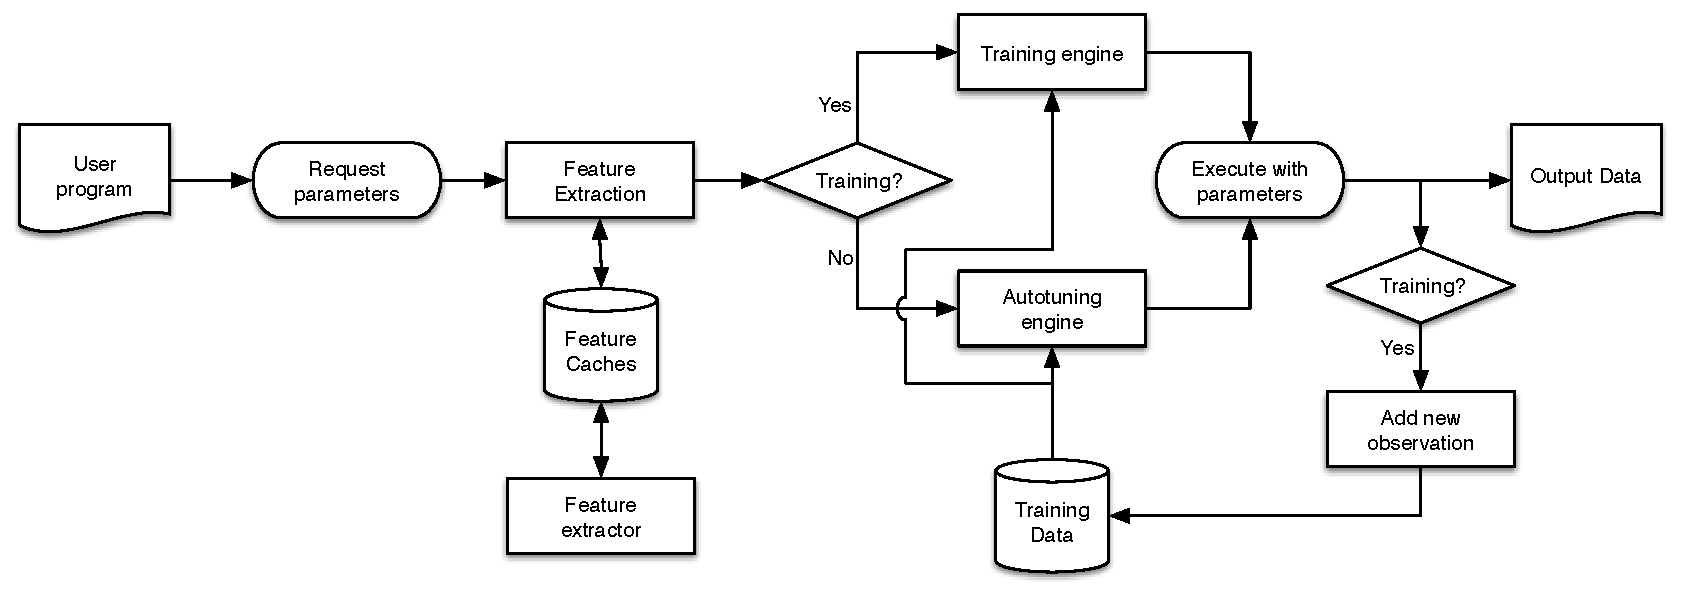
\includegraphics[width=\columnwidth]{img/omnitune-system-flow.pdf}
\caption[Optimisation parameter selection with OmniTune]{%
  The process of selecting optimisation parameter values for a given
  user program with OmniTune.%
}
\label{fig:omnitune-system-flow}
\end{figure}

The goal of machine learning-enabled autotuning is to \emph{predict}
the values for optimisation parameters to maximise some measure of
profit. These predictions are based on models built from prior
observations. The prediction quality is influenced by the number of
prior observations. OmniTune supports both prediction of parameters
based on prior observations, and a method for collecting these
observations. When a client program requests parameter values, it
indicates whether the request is for training or performance purposes,
and uses a different backend to select parameter values for each. New
observations can then be added once parameters have been evaluated.
Figure~\ref{fig:omnitune-system-flow} shows this process.


\subsection{System Architecture and Interface}

\begin{figure}
\centering
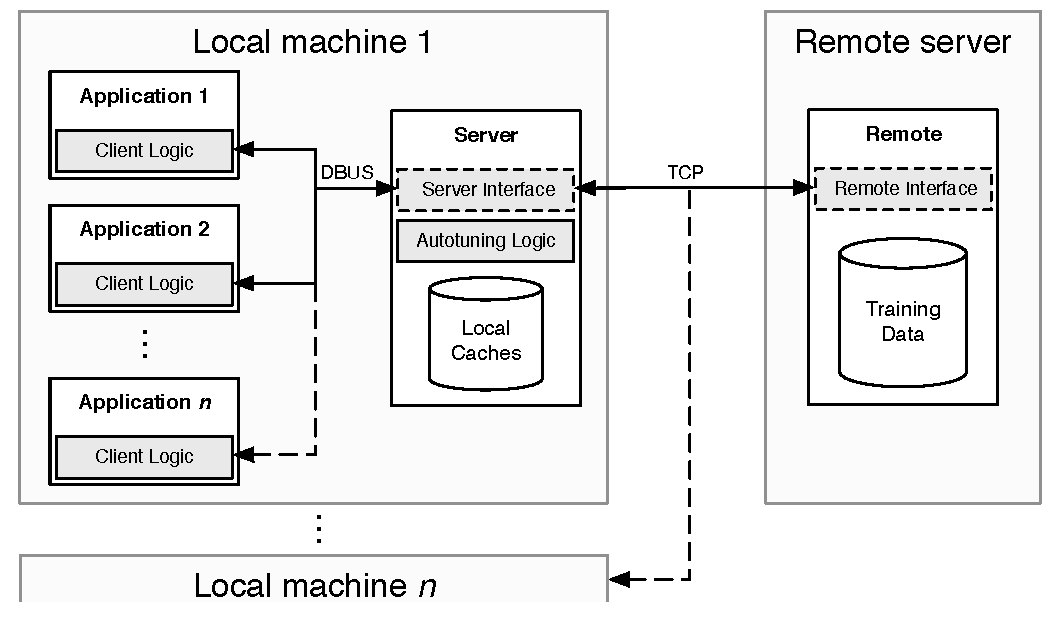
\includegraphics[width=.9\columnwidth]{img/omnitune-system-overview.pdf}
\caption[OmniTune system diagram]{%
  High level overview of OmniTune components.%
}
\label{fig:omnitune-system-overview}
\end{figure}

Common implementations of autotuning in the literature either: embed
the autotuning logic within the each target application, or take a
standalone approach in which the autotuner is a program which must be
invoked by the user to tune a target application. Embedding the
autotuner within each target application has the advantage of
providing ``always-on'' behaviour, but is infeasible for complex
systems in which the cost of building machine learning models must be
added to each program run. The standalone approach separates the
autotuning logic, at the expense of adding one additional step to the
build process. The approach taken in OmniTune aims to capture the
advantages of both techniques by implementing a autotuning \emph{as a
  service}, with only the lightweight communication logic embedded in
the target applications.

Omnitune is built around a three tier client-server model. The
applications which are to be autotuned are the \emph{clients}. These
clients commmunicate with a system-wide \emph{server}, which handles
autotuning requests. The server communicates and caches data sourced
from a \emph{remote}, which maintains a global store of all autotuning
data. Figure~\ref{fig:omnitune-system-overview} shows this structure.

There is a many to one relationship between clients, servers, and
remotes, such that a single remote may handle connections to multiple
servers, which in turn may accept connections from multiple
clients. This design has two primary advantages: the first is that it
decouples the autotuning logic from that of the client program,
allowing developers to easily repurpose the autotuning framework to
target additional optimisation parameters without a significant
development overhead for the target applications; the second advantage
is that this enables collective tuning, in which training data
gathered from a range of devices can be accessed and added to by any
OmniTune server.

OmniTune supports autotuning using a separate offline training phase,
online training, or a mixture of both. Figure~\ref{fig:omnitune-comms}
shows an example pattern of communication between the three tiers of
an OmniTune system, showing a distinct training phase. Note that this
training phase is enforced only by the client. The following sections
describe the interfaces between the three components.


\begin{figure}
\centering
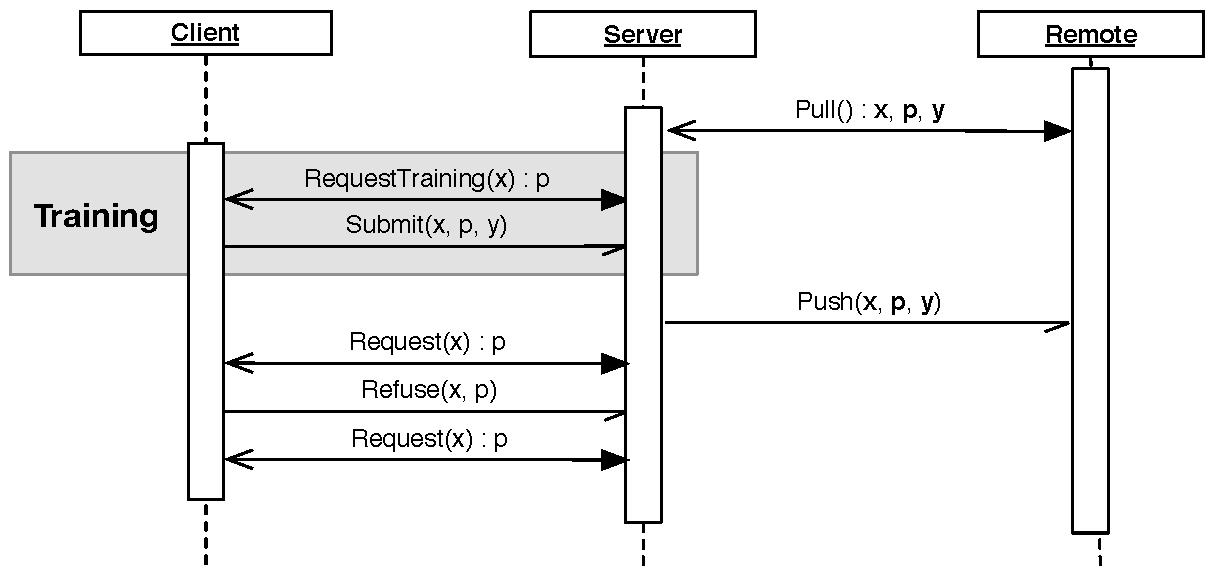
\includegraphics[width=1.0\columnwidth]{img/omnitune-comms}
\caption[Communication pattern between OmniTune components]{%
  An example communication pattern between OmniTune components,
  showing an offline training phase.%
}
\label{fig:omnitune-comms}
\end{figure}


\subsubsection{Client Interface: Lightweight Communication}

Client applications communicate with an OmniTune server through four
operations:
%
\begin{itemize}
\item \textsc{Request}$(x) \to p$ Given a set of explanatory variables
  $x$, request a set of parameter values $p$ to maximise performance.
\item \textsc{RequestTraining}$(x) \to p$ Given a set of explanatory
  variables $x$, allow the server to select a set of parameter values
  $p$ for evaluating their fitness.
\item \textsc{Submit}$(x, p, y)$ Submit an observed measurement of
  fitness $y$ of parameters $p$, given explantory variables $x$.
\item \textsc{Refuse}$(x, p)$ Refuse a set of parameters $p$ given a
  set of explanatory variables $x$. Once refused, those parameters
  will not be returned by any subsequent calls to \textsc{Request()}
  or \textsc{RequestTraining()}.
\end{itemize}
%
This set of operations enables the core functionality of an autotuner,
while providing flexibility for the client to control how and when
training data is collected.


\subsubsection{Server: Autotuning Engine}

For each autotuning-capable machine, a system-level daemon hosts a
DBus session bus which client processes communicate with. This daemon
acts as an intermediate between the training data and the client
applications, \emph{serving} requests for optimisation parameter
values. Servers operations are application-specific, so there is a set
of operations to implement autotuning of each supported optimisation
target.

The server is implemented as a standalone Python program, and contains
a library of machine learning tools to perform parameter prediction,
interfacing with Weka using the JNI. Weka is a suite of data mining
software developed by the University of Waikato, freely available
under the GNU GPL
license~\footnote{http://www.cs.waikato.ac.nz/ml/weka/}. OmniTune
servers may perform additional feature extraction of explanatory
variables supplied by incoming client requests. The reason for
performing feature extraction on the server as opposed to on the
client side is that this allows the results of expensive operations
(for example, analysing source code of target applications) to be
cached for use across the lifespan of client applications. The
contents of these local caches are periodically and asynchronously
synced with the remote, to maintain a global store of lookup tables
for expensive operations.

On launch, the server requests the latest training data from the
remote, which it uses to build the relevant models for performing
prediction of optimisation parameter values. Servers communicate with
remotes by submitting or requesting training data in batches, using
two operations:
%
\begin{itemize}
\item \textsc{Push}$(\bf{f}, \bf{c})$ Submit a set of labelled training
  points as pairs $(f,c)$.
\item \textsc{Pull}$() \to (\bf{f}, \bf{c})$ Request training data as a
  set of labelled $(f,c)$ pairs.
\end{itemize}


\subsubsection{Remote: Distributed Training Data}

The role of the remote is to provide bookkeeping of training data for
machine learning. Using the interface described in the previous
subsection, remotes allow shared access to data from multiple servers
using a transactional communication pattern.


\subsection{Summary}

This section has described the architecture of of OmniTune, a
distributed autotuner which is capable of performing runtime
prediction of optimal workgroup sizes using a variety of machine
learning approaches. OmniTune uses a client-server model to decouple
the autotuning logic from target programs and to maintain separation
of concerns. It uses lightweight inter-process communication to
achieve low latency autotuning, and uses caches and lookup tables to
minimise the one-off costs of feature extraction.



\section{Autotuning SkelCL Stencils}\label{sec:omnitune-skelcl}

In this section I apply the OmniTune framework to SkelCL. The publicly
available implementation
\footnote{\url{https://github.com/ChrisCummins/omnitune}} predicts
workgroup sizes for OpenCL stencil skeleton kernels in order to
minimise their runtime on CPUs and multi-GPU systems. The optimisation
space presented by the workgroup size of OpenCL kernels is large,
complex, and non-linear. Successfully applying machine learning to
such a space requires plentiful training data, the careful selection
of features, and classification approach. The following subsections
address these challenges.


% Anyone downloading a copy of OmniTune will instantly have access to
% the global database of training data, including the
% \input{gen/num_samples} runtimes which were collected to write this
% thesis.

% \texttt{cec.chlox1mra3iz.us-west-2.rds.amazonaws.com:3306}

\subsection{Training}\label{subsec:training}

One challenge of performing empirical performance evaluations is
gathering enough applications to ensure meaningful
comparisons. Synthetic benchmarks are one technique for circumventing
this problem. The automatic generation of such benchmarks has clear
benefits for reducing evaluation costs; however, creating meaningful
benchmark programs is a difficult problem if we are to avoid the
problems of redundant computation and produce provable halting
benchmarks.

In practise, stencil codes exhibit many common traits: they have a
tightly constrained interface, predictable memory access patterns, and
well defined numerical input and output data types. This can be used
to create a confined space of possible stencil codes by enforcing
upper and lower bounds on properties of the codes which can not
normally be guaranteed for general-purpose programs, e.g.\ the number
of floating point operations. In doing so, it is possible to
programatically generate stencil workloads which share similar
properties to those which we intend to target.

Based on observations of real world stencil codes from the fields of
cellular automata, image processing, and PDE solvers, I implemented a
stencil generator which uses parameterised kernel templates to produce
source codes for collecting training data. The stencil codes are
parameterised by stencil shape (one parameter for each of the four
directions), input and output data types (either integers, or single
or double precision floating points), and \emph{complexity} --- a
simple boolean metric for indicating the desired number of memory
accesses and instructions per iteration, reflecting the relatively
bi-modal nature of the reference stencil codes, either compute
intensive (e.g. FDTD simulations), or lightweight (e.g. Game of Life).

Using a large number of synthetic benchmarks helps adress the ``small
$n$, large $P$'' problem, which describes the difficulty of
statistical inference in spaces for which the set of possible
hypotheses $P$ is significantly larger than the number of observations
$n$. By creating parameterised, synthetic benchmarks, it is possible
to explore a much larger set of the space of possible stencil codes
than if relying solely on reference applications, reducing the risk of
overfitting to particular program features.


\subsection{Stencil Features}


\begin{table}
  \scriptsize
  \centering
  \begin{tabular}{p{5cm}p{1.5cm}}
    \toprule
    \textbf{Dataset Features} &         \textbf{Type} \\
    \midrule
    Number of columns in matrix & numeric \\
    Number of rows in matrix & numeric \\
    Input data type & categorical \\
    Output data type & categorical \\
    \bottomrule
  \end{tabular}
\caption{OmniTune SkelCL Stencil features for datasets.}
\label{tab:features-datasets}
\end{table}

\begin{table}
  \scriptsize
  \centering
  \begin{tabular}{p{5cm}p{1.5cm}}
    \toprule
    \textbf{Kernel Features} &         \textbf{Type} \\
    \midrule
    Border region north &      numeric \\
    Border region south &      numeric \\
    Border region east &      numeric \\
    Border region west &      numeric \\
    Static instruction count &      numeric \\
    \texttt{AShr} instruction density &      numeric \\
    \texttt{Add} instruction density &      numeric \\
    \texttt{Alloca} instruction density &      numeric \\
    \texttt{And} instruction density &      numeric \\
    \texttt{Br} instruction density &      numeric \\
    \texttt{Call} instruction density &      numeric \\
    \texttt{FAdd} instruction density &      numeric \\
    \texttt{FCmp} instruction density &      numeric \\
    \texttt{FDiv} instruction density &      numeric \\
    \texttt{FMul} instruction density &      numeric \\
    \texttt{FPExt} instruction density &      numeric \\
    \texttt{FPToSI} instruction density &      numeric \\
    \texttt{FSub} instruction density &      numeric \\
    \texttt{GetElementPtr} instruction density  &      numeric \\
    \texttt{ICmp} instruction density &      numeric \\
    \texttt{InsertValue} instruction density &      numeric \\
    \texttt{Load} instruction density &      numeric \\
    \texttt{Mul} instruction density &      numeric \\
    \texttt{Or} instruction density &      numeric \\
    \texttt{PHI} instruction density &      numeric \\
    \texttt{Ret} instruction density &      numeric \\
    \texttt{SDiv} instruction density &      numeric \\
    \texttt{SExt} instruction density &      numeric \\
    \texttt{SIToFP} instruction density &      numeric \\
    \texttt{SRem} instruction density &      numeric \\
    \texttt{Select} instruction density &      numeric \\
    \texttt{Shl} instruction density &      numeric \\
    \texttt{Store} instruction density &      numeric \\
    \texttt{Sub} instruction density &      numeric \\
    \texttt{Trunc} instruction density &      numeric \\
    \texttt{UDiv} instruction density &      numeric \\
    \texttt{Xor} instruction density &      numeric \\
    \texttt{ZExt} instruction density &      numeric \\
    Basic block density & numeric \\
    Memory instruction density & numeric \\
    Non external functions density &      numeric \\
    Kernel max workgroup size &      numeric \\
    \bottomrule
  \end{tabular}
\caption{OmniTune SkelCL Stencil features for kernels.}
\label{tab:features-kernels}
\end{table}

\begin{table}
  \scriptsize
  \centering
  \begin{tabular}{p{5cm}p{1.5cm}}
    \toprule
    \textbf{Device Features} &         \textbf{Type} \\
    \midrule
    SkelCL device count &      numeric \\
    Device address width &  categorical \\
    Double precision fp.\ configuration &  categorical \\
    Big endian? &  categorical \\
    Execution capabilities &  categorical \\
    Supported extensions &  categorical \\
    Global memory cache size &  numeric \\
    Global memory cache size &      categorical \\
    Global memory cacheline size &      numeric \\
    Global memory size &  numeric \\
    Host unified memory? &      categorical \\
    2D image max height &      numeric \\
    2D image max width &      numeric \\
    3D image max depth &      numeric \\
    3D image max height &      numeric \\
    3D image max width &  numeric \\
    Image support &      categorical \\
    Local memory size &  numeric \\
    Local memory type &      categorical \\
    Max clock frequency &      numeric \\
    Number of compute units &      numeric \\
    Max kernel constant args &      numeric \\
    Max constant buffer size &      numeric \\
    Max memory allocation size &      numeric \\
    Max parameter size &      numeric \\
    Max read image arguments &      numeric \\
    Max samplers &      numeric \\
    Max device workgroup size &      numeric \\
    Max workitem dimensions &      numeric \\
    Max work item sizes width &      numeric \\
    Max work item sizes height &      numeric \\
    Max work item sizes depth &      numeric \\
    Max write image arguments &      numeric \\
    Mem base address align &      numeric \\
    Min data type align size &      numeric \\
    Native vector width \texttt{char} &      numeric \\
    Native vector width \texttt{double} &      numeric \\
    Native vector width \texttt{float} &      numeric \\
    Native vector width \texttt{half} &      numeric \\
    Native vector width \texttt{int} &      numeric \\
    Native vector width \texttt{long} &      numeric \\
    Native vector width \texttt{short} &      numeric \\
    Preferred vector width \texttt{char} &      numeric \\
    Preferred vector width \texttt{double} &      numeric \\
    Preferred vector width \texttt{float} &      numeric \\
    Preferred vector width \texttt{half} &      numeric \\
    Preferred vector width \texttt{int} &      numeric \\
    Preferred vector width \texttt{long} &      numeric \\
    Preferred vector width \texttt{short} &  categorical \\
    Queue properties &  categorical \\
    Single precision fp.\ configuration &  categorical \\
    Device type &      categorical \\
    OpenCL vendor &  categorical \\
    OpenCL vendor ID &  categorical \\
    OpenCL version &  categorical \\
    \bottomrule
  \end{tabular}
\caption{OmniTune SkelCL Stencil features for devices.}
\label{tab:features-devices}
\end{table}


Properties of the architecture, program, and dataset all contribute to
the performance of a workgroup size. The success of a machine learning
system depends on the ability to translate these properties into
meaningful explanatory variables --- \emph{features}. To capture this
in OmniTune, parameter requests are packed with a copy of the OpenCL
kernel and attributes of the dataset and device. The OmniTune server
extracts 102 features describing hte architecture, kernel, and dataset
from the message:
%
\begin{itemize}
\item \textbf{Device} --- OmniTune uses the OpenCL
  \texttt{clGetDeviceInfo()} API to query a number of properties about
  the target execution device. Examples include the size of local
  memory, maximum work group size, number of compute units, etc.
\item \textbf{Kernel} --- The user code for a stencil is passed to the
  OmniTune server, which compiles the OpenCL kernel to LLVM IR
  bitcode. The \texttt{opt} \texttt{InstCount} statistics pass is used
  to obtain static counts for each type of instruction present in the
  kernel, as well as the total number of instructions. The instruction
  counts for each type are divided by the total number of instructions
  to produce a \emph{density} of instruction for that type. Examples
  include total static instruction count, ratio of instructions per
  type, ratio of basic blocks per instruction, etc.
\item \textbf{Dataset} --- The SkelCL container type is used to
  extract the input and output data types, and the 2D grid size.
\end{itemize}
%
See Tables~\ref{tab:features-datasets},~\ref{tab:features-kernels},
and~\ref{tab:features-devices} for a list of feature names and types.


\subsubsection{Reducing Feature Extraction Overhead}


Feature extraction (particularlly compilation to LLVM IR) introduces a
runtime overhead to the classification process. To minimise this,
lookup tables for device and dataset features are used, and cached
locally in the OmniTune server and pushed to the remote data
store. The device ID is used to index the devices table, and the
checksum of an OpenCL source is used to index the kernel features
table. Before feature extraction for either occurs, a lookup is
performed in the relevant table, meaning that the cost of feature
extraction is amortised over time.


\subsection{Optimisation Parameters}\label{subsec:op-params}

SkelCL stencil kernels are parameterised by a workgroup size $w$,
which consists of two integer values to denote the number of rows and
columns (where we need to distinguish the individual components, we
will use symbols $w_r$ and $w_c$ to denote rows and columns,
respectively).


\subsubsection{Constraints}

Unlike in many autotuning applications, the space of optimisation
parameter values is subject to hard constraints, and these constraints
cannot conviently be statically determined. Contributing factors are
architectural limitations, kernel constraints, and refused parameters.


\paragraph{Architectural constraints}

Each OpenCL device imposes a maximum workgroup size which can be
statically checked by querying the \texttt{clGetDeviceInfo()} API for
that device. These are defined by archiectural limitations of how code
is mapped to the underlying execution hardware. Typical values are
powers of two, e.g.\ 1024, 4096, 8192.


\paragraph{Kernel constraints}

At runtime, once an OpenCL program has been compiled to a kernel,
users can query the maximum workgroup size supported by that kernel
using the \texttt{clGetKernelInfo()} API. This value cannot easily be
obtained statically as there is no mechanism to determine the maximum
workgroup size for a given source code and device without first
compiling it, which in OpenCL does not occur until runtime. Factors
which affect a kernel's maximum workgroup size include the number
registers required for a kernel, and the available number of SIMD
execution units for each type of instructions in a kernel.


\paragraph{Refused parameters}

In addition to satisfying the constraints of the device and kernel,
not all points in the workgroup size optimisation space are guaranteed
to provide working programs. A refused parameter is a workgroup size
which satisfies the kernel and architectural constraints, yet causes a
\texttt{CL\_OUT\_OF\_RESOURCES} error to be thrown when the kernel is
enqueued. Note that in many OpenCL implementations, this error type
acts as a generic placeholder and may not necessarily indicate that
the underlying cause of the error was due to finite resources
constraints.


\paragraph{Legality}

We define a \emph{legal} workgroup size as one which, for a given
\emph{scenario} (a combination of program, device, and dataset),
satisfies the architectural and kernel constraints, and is not
refused. The subset of all possible workgroup sizes
$W_{legal}(s) \subset W$ that are legal for a given sceanario $s$ is
then:
%
\begin{equation}
  W_{legal}(s) = \left\{w | w \in W, w < W_{\max}(s) \right\} - W_{refused}(s)
\end{equation}
%
Where $W_{\max}(s)$ can be determined at runtime prior to the kernels
execution, but the set $W_{refused}(s)$ can only be determined
experimentally.


\subsubsection{Assessing Relative Performance}

Given a set of observations, where an observation is a scenario,
workgroup size tuple $(s,w)$; a function $t(s,w)$ which returns the
arithmetic mean of the runtimes for a set of observations; we can
calculate the speedup $r(s, w_1, w_2)$ of competing workgroup sizes
$w_1$ over $w_2$ using:
%
\begin{equation}
  r(s, w_1, w_2) = \frac{t(s,w_2)}{t(s,w_1)}\\
\end{equation}
%

\paragraph{Oracle Workgroup Size}

The \emph{oracle} workgroup size $\Omega(s) \in W_{legal}(s)$ of a
sceanrio $s$ is the $w$ value which provides the lowest mean
runtime. This allows for comparing the performance $p(s,w)$ of a
particular workgroup against the maximum available performance for
that scenario, within the range $0 \le p(s,w) \le 1$:

\begin{align}
  \Omega(s) &= \argmin_{w \in W_{legal}(s)} t(s,w)\\
  p(s,w) &= r(s, w, \Omega(s))
\end{align}


\paragraph{Establishing a Baseline}

The geometric mean is used to aggregate normalised relative
performances due to its multiplicative
property~\cite{Fleming1986}. For a given workgroup size, the average
performance $\bar{p}(w)$ across the set of all scenarios $S$ can be
found using the geometric mean of performance relative to the oracle:
%
\begin{equation}
\bar{p}(w) =
\left(
  \prod_{s \in S} r(s, w, \Omega(s))
\right)^{1/|S|}
\end{equation}
%
The \emph{baseline} workgroup size $\bar{w}$ is the value which
provides the best average case performance across all scenarios. Such
a baseline value represents the \emph{best} possible performance which
can be achieved using a single, statically chosen workgroup size. By
defining $W_{safe} \in W$ as the intersection of legal workgroup
sizes, the baseline can be found using:

\begin{align}
W_{safe} &= \cap \left\{ W_{legal}(s) | s \in S \right\}\\
\bar{w} &= \argmax_{w \in W_{safe}} \bar{p}(w)
\end{align}


\subsection{Machine Learning}

The challenge is to design a system which, given a set of prior
observations of the empirical performance of stencil codes with
different workgroup sizes, predict workgroup sizes for \emph{unseen}
stencils which will maximise the performance. The OmniTune server
supports three methods for achieving this.


\subsubsection{Predicting Oracle Workgroup Size}

The first approach to predicting workgroup sizes is to consider the
set of possible workgroup sizes as a hypothesis space, and to use a
classifier to predict, for a given set of features, the workgroup size
which will provide the best performance. The classifier takes a set of
training scenarios $S_{training}$, and generates labelled training
data as pairs of scenario features $f(s)$ and observed oracle
workgroup sizes:
%
\begin{equation}
  T = \left\{ \left(f(s), \Omega(s)\right) | s \in S_{training} \right\}
\end{equation}
%
During testing, the classifier predicts workgroup sizes from the set
of oracle workgroup sizes from the training set:
%
\begin{equation}
  W_{training} = \left\{ \Omega(s) | s \in S_{training} \right\}
\end{equation}
%
This approach presents the problem that after training, there is no
guarantee that the set of workgroup sizes which may be predicted is
within the set of legal workgroup sizes for future scenarios:
%
\begin{equation}
  \bigcup_{\forall s \in S_{testing}} W_{legal}(s) \nsubseteq W_{training}
\end{equation}
%
This may result in a classifier predicting a workgroup size which is
not legal for a scenario, $w \not\in W_{legal}(s)$, either because it
exceeds $W_{\max}(s)$, or because the parameter is refused. For these
cases, I evaluate the effectiveness of three fallback strategies to
select a legal workgroup size:
%
\begin{enumerate}
\item \emph{Baseline} --- select the workgroup size which is known to
  be safe $w < W_{safe}$, and provides the highest average case
  performance on training data.
\item \emph{Random} --- select a random workgroup size which is known
  from prior observations to be legal $w \in W_{legal}(s)$.
\item \emph{Nearest Neighbour} --- select the workgroup size which
  from prior observations is known to be legal, and has the lowest
  Euclidian distance to the prediction.
\end{enumerate}
%
See Algorithm~\ref{alg:autotune-classification} for definitions.

\begin{algorithm}
\begin{algorithmic}[1]
\Require scenario $s$
$d$.
\Ensure workgroup size $w$

\Procedure{Baseline}{s}
\Comment Select the best $w$ from $W_{safe}$.
\State $w \leftarrow \text{classify}(f(s))$
\If{$w \in W_{legal}(s)$}
    \State \textbf{return} $w$
\Else
  \State \textbf{return} $\underset{w \in W_{safe}}{\argmax}
\left(
  \prod_{s \in S_{training}} p(s, w)
\right)^{1/|S_{training}|}$
\EndIf
\EndProcedure
\item[] % line break

\Procedure{Random}{s}
\Comment Select a random workgroup size.
\State $w \leftarrow \text{classify}(f(s))$
\While{$w \not\in W_{legal}(s)$}
  \State $w \leftarrow $ random selection $w \in \left\{ w | w < W_{max}(s), w \not\in W_{refused}(s) \right\}$
\EndWhile
\State \textbf{return} $w$
\EndProcedure
\item[] % line break

\Procedure{NearestNeighbour}{s}
\Comment Select the closest workgroup size to prediction.
\State $w \leftarrow \text{classify}(f(s))$
\While{$w \not\in W_{legal}(s)$}
  \State $d_{min} \leftarrow \infty$
  \State $w_{closest} \leftarrow \text{null}$
  \For{$c \in \left\{ w | w < W_{\max}(s), w \not\in W_{refused}(s) \right\}$}
    \State $d \leftarrow \sqrt{\left(c_r - w_r\right)^2 + \left(c_c - w_c\right)^2}$
    \If{$d < d_{min}$}
      \State $d_{min} \leftarrow d$
      \State $w_{closest} \leftarrow c$
    \EndIf
  \EndFor
  \State $w \leftarrow w_{closest}$
\EndWhile
\State \textbf{return} $w$
\EndProcedure
\end{algorithmic}
\caption{Selecting optimal workgroup sizes using classification}
\label{alg:autotune-classification}
\end{algorithm}

\subsubsection{Predicting Stencil Code Runtime}

\begin{algorithm}
\begin{algorithmic}[1]
\Require kernel features $k$, hardware features $h$, dataset features
$d$.
\Ensure workgroup size $w$

\State $W \leftarrow \left\{ w | w < W_{\max}(s) \right\} - W_{refused}(s)$
\Comment Set of possible workgroup sizes.
\State $w \leftarrow \underset{w \in W}{\argmin} g(f(s), w)$
\Comment Predict candidate workgroup size.
\While{$w \not\in W_{legal}(s)$}
  \State $W \leftarrow W - \left\{ w \right\}$
  \Comment Remove candidate from set.
  \State $w \leftarrow \underset{w \in W}{\argmin} g(f(s), w)$
  \Comment Select next candidate workgroup size.
\EndWhile
\State \textbf{return} $w$
\end{algorithmic}
\caption{Selecting workgroup sizes by predicting program runtimes}
\label{alg:autotune-runtime-regression}
\end{algorithm}

A problem of predicting oracle workgroup sizes is that it requires
each training point to be labelled with the oracle workgroup size
which can be only be evaluated using an exhaustive search. An
alternative approach is to build a model to attempt to predict the
\emph{runtime} of a stencil given a specific workgroup size. This
allows for training on data for which the oracle workgroup size is
unknown, and has the secondary advantage that this allows for an
additional training data point to be gathered each time a stencil is
evaluated. Given training data consisting of $(f(s),w,t)$ tuples,
where $s$ is a scenario, $w$ is the workgroup size, and $t$ is the
observed mean runtime, we can train a regressor $g(f(s), w)$ which
predicts the mean runtime of an unseen scenario. The predicted oracle
workgroup size $\bar{\Omega}(s)$ is then the $w$ value which minimises
the output of the regressor:
%
\begin{equation}
  \bar{\Omega}(s) = \underset{w \in W_{legal}(s)}{\argmin} g(f(s), w)
\end{equation}
%
Note that since we cannot know in advance which workgroup sizes will
be refused, that is, $W_{refused}(s)$ cannot be statically determined,
this process must be iterated until a workgroup size which not refused
is selected. Algorithm~\ref{alg:autotune-runtime-regression} shows
this process.


\subsubsection{Predicting Relative Performance of Workgroup Sizes}

\begin{algorithm}
\begin{algorithmic}[1]
\Require kernel features $k$, hardware features $h$, dataset features
$d$, baseline $w_b$.
\Ensure workgroup size $w$

\State $W \leftarrow \left\{ w | w < W_{\max}(s) \right\} - W_{refused}(s)$
\Comment Set of possible workgroup sizes.
\State $w \leftarrow \underset{w \in W}{\argmax} g(f(s), w,w_b)$
\Comment Predict candidate workgroup size.
\While{$w \not\in W_{legal}(s)$}
  \State $W \leftarrow W - \left\{ w \right\}$
  \Comment Remove candidate from set.
  \State $w \leftarrow \underset{w \in W}{\argmax} g(f(s), w,w_b)$
  \Comment Select next candidate workgroup size.
\EndWhile
\State \textbf{return} $w$
\end{algorithmic}
\caption{Selecting workgroup sizes by predicting relative performance}
\label{alg:autotune-speedup-regression}
\end{algorithm}

Accurately predicting the runtime of an arbitrary program is a
difficult problem due to the impacts of flow control. In such cases,
it may be more effective to instead predict the \emph{relative}
performance of two different workgroup sizes for the same program. To
do this, we select a baseline workgroup size $w_b \in W_{safe}$, and
train a regressor $g(f(s),w,w_b)$ with training data labelled with the
relative performance over the baseline $r(w, w_b)$. Predicting the
optimal workgroup requires maximising the output of the regressor:
%
\begin{equation}
  \bar{\Omega}(s) = \underset{w \in W_{legal}(s)}{\argmax} g(f(s),w,w_b)
\end{equation}
%
As with predicting runtimes, this process must be iterated to
accommodate for the emergent properties of $W_{legal}(s)$. See
Algorithm~\ref{alg:autotune-speedup-regression} for a description of
this process.


\subsection{Implementation}

The OmniTune framework is implemented as a set of Python classes and
interfaces, which are inherited from or implemented to target specific
autotuning cases. The entire framework consists of 8987 lines of
Python code, of which 976 is dedicated to the SkelCL frontend. By
design, the client-server model minimises the impact of number of
modifications that are required to enable autotuning in client
applications. The only modification required is to replace the
hardcoded values for workgroup size with a subroutine to request a
workgroup size from the OmniTune server over a DBUS connection. The
server is implemented as a standalone Python program, and uses sqlite
to maintain local data caches. The OmniTune remote is an Amazon Web
Services virtual machine instance, using MySQL as the relational data
store. Figure~\ref{fig:omnitune-system-flow} shows the relational
database schema used to store stencil runtime information. Additional
tables store data in coalesced forms for use as machine learning
training data.

For classification, five classifiers are supported, chosen for their
contrasting properties: Naive Bayes, SMO, Logistic Regression, J48
Decision tree, and Random Forest. For regression, a Random Forest with
regression trees is used, chosen because of its efficient handling of
large feature sets, compared to linear models.

\begin{figure}
\centering
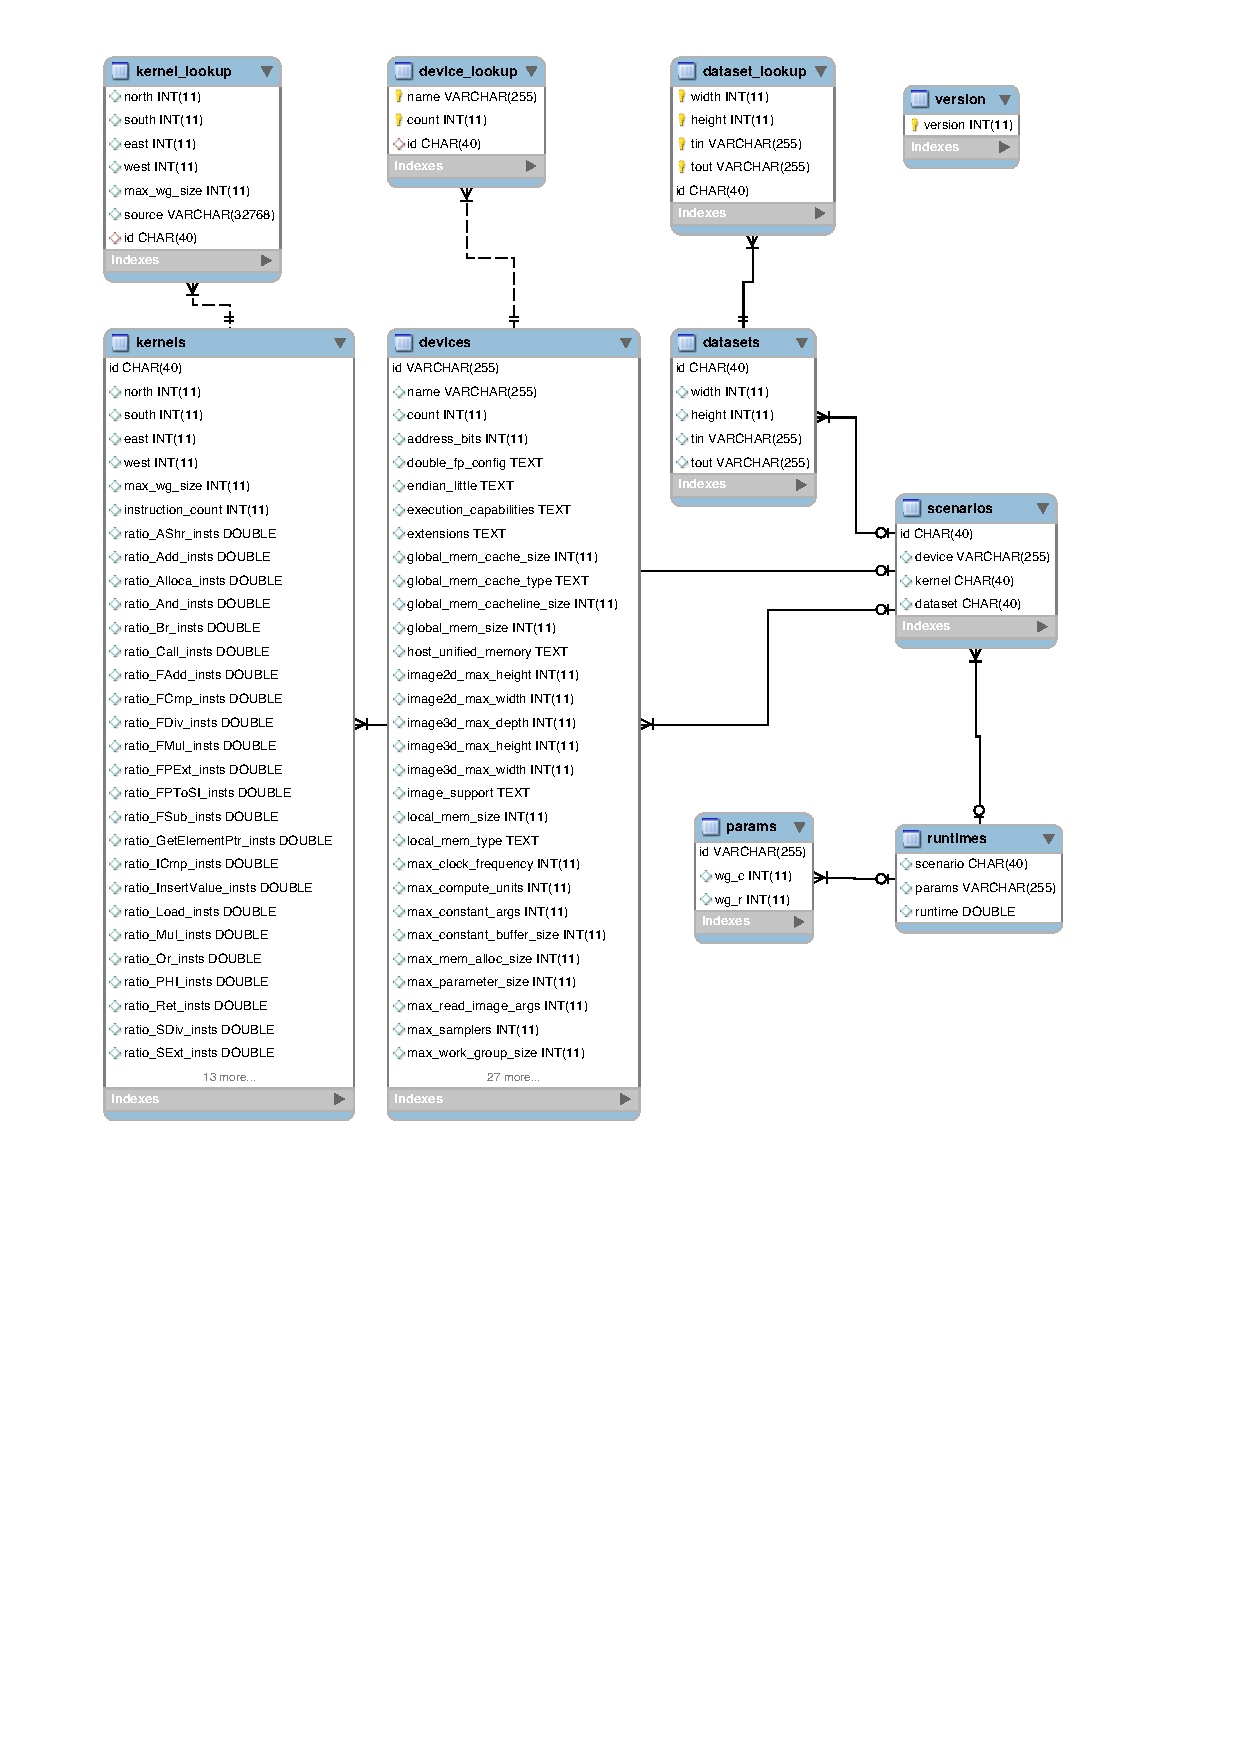
\includegraphics[width=.95\columnwidth]{img/omnitune-data-schema.pdf}
\caption[Database schema for storing performance results]{%
  Database schema for storing SkelCL stencil runtimes. Feature lookup
  tables and normalisation are used to provide extremely compact
  storage, requiring only 56 bytes for each additional runtime of a
  known stencil program.%
}
\label{fig:omnitune-system-flow}
\end{figure}


\subsection{Summary}

This section has described has the application of OmniTune for
predicting workgroup sizes of SkelCL stencil programs, using three
different machine learning approaches. The first approach is to
predict the optimal workgroup size for a given program based on
training data which included the optimal workgroup sizes for other
stencils. The second approach is to select a workgroup sizex by
sweeping the space of possible workgroup sizes, predicting the runtime
a program with each. The third approach is to select a workgroup size
by sweeping the space of possible workgroup sizes, predicting the
relative gain of each compared to a known baseline. In the next
section, we will describe the process for collecting empirical
performance data.



\section{Methodology}\label{sec:methodology}

This section describes an exhaustive enumeration of the workgroup size
optimisation space for 429 combinations of architecture, program, and
dataset. It contains the methodology used to collect empirical
performance data on which to base performance comparisons of different
workgroup sizes, and the steps necessary to obtain repeatable results.


\subsection{Experimental Setup}

\begin{table}
\scriptsize
\centering
\begin{tabular}{lllp{.95cm}}
\toprule
  Processor & Memory & OpenCL Devices & OpenCL Version \\
\midrule
  Intel i7-2600 &   8 GB &                Nvidia GTX TITAN &  1.1 \\
 Intel i7-2600K &  16 GB &                  Nvidia GTX 690 &  1.1 \\
  Intel i7-3820 &   8 GB &         $4\times$Nvidia GTX 590 &  1.1 \\
  Intel i7-3820 &   8 GB &   CPU, $2\times$AMD Tahiti 7970 &  1.2 \\
  Intel i5-4570 &   8 GB &                             CPU &  1.2 \\
 Intel i5-2430M &   8 GB &                             CPU &  1.2 \\
\bottomrule
\end{tabular}
\caption[Specification of experimental platforms]{%
  Specification of experimental platforms.%
}
\label{tab:hosts}
\end{table}

Table~\ref{tab:hosts} describes the experimental platforms used.  All
runtimes were recorded with millisecond precision using either the
system clock or OpenCL's Profiling API. Measurement noise was
minimised by reducing system load through disabling all unwanted
services and graphical environments, and exclusive single-user access
was ensured for each platform. Frequency governors for each CPU were
disabled, and the benchmark processes were set to the highest priority
available to the task scheduler. Datasets and programs were stored in
an in-memory file system.

\subsubsection{Devices}

\begin{table*}
\scriptsize
\centering
\begin{tabular}{lp{1cm}lp{1.2cm}p{1cm}p{1.3cm}}
\toprule
             Name &  Compute units & Frequency & Local Memory & Global Cache & Global Memory \\
\midrule
  AMD Tahiti 7970 &             32 &   1000 Hz &        32 KB &        16 KB &       2959 MB \\
   Intel i5-2430M &              4 &   2400 Hz &        32 KB &       256 KB &       7937 MB \\
    Intel i5-4570 &              4 &   3200 Hz &        32 KB &       256 KB &       7901 MB \\
    Intel i7-3820 &              8 &   1200 Hz &        32 KB &        32 KB &       7944 MB \\
   Nvidia GTX 590 &              1 &   1215 Hz &        48 KB &       256 KB &       1536 MB \\
   Nvidia GTX 690 &              8 &   1019 Hz &        48 KB &       128 KB &       2048 MB \\
 Nvidia GTX TITAN &             14 &    980 Hz &        48 KB &       224 KB &       6144 MB \\
\bottomrule
\end{tabular}
\caption[Specification of experimental OpenCL devices]{%
  Specification of experimental OpenCL devices.%
}
\label{tab:hw}
\end{table*}

Table~\ref{tab:hw} describes the OpenCL devices used for testing, as
available on the experimental platforms.

\subsubsection{Benchmark Applications}

In addition to the synthetic stencil benchmarks described in
Subsection~\ref{subsec:training}, six stencil kernels taken from four
reference implementations of standard stencil applications from the
fields of image processing, cellular automata, and partial
differential equation solvers are used:
%
\begin{itemize}
\item \textbf{Game of Life} Conway's Game of Life~\cite{Conway1970} is
  a cellular automaton which models the evolution of a regular grid of
  cells over discrete time steps. At each time step, each cell value
  is updated to be either \emph{live} or \emph{dead} based on it's
  current state and the state of the one immediately neighbouring cell
  to the north, south, east, and west.
\item \textbf{Heat Equation} The heat equation is a partial
  differential equation which describes the distribution of heat in a
  given region over time. Each iteration of the stencil represents a
  discrete time step, and the value of each cell (i.e.\ the
  temperature) is smoothed based on the temperatures of surrounding
  cells and the thermal conductivity of the material being simulated.
\item \textbf{Gaussian Blur} The Gaussian blur is a common image
  processing algorithm, used to reduce noise and detail in an image. A
  two dimensional Gaussian blur defines a function to compute a pixel
  value based on the value of neighbouring pixels. Gaussian blurs are
  parameterised by a radius which define symmetric, square stencil
  regions about the centre pixel. Unlike the previous two
  applications, the Gaussian blur is not an iterative stencil.
\item \textbf{Canny Edge Detection} The Canny edge detection algorithm
  is a multi-stage approach to detecting edges in
  images~\cite{Canny1986}. It consists of four distinct stages: a
  noise reduction operation, an edge detection operation, a
  non-maximum suppression, and a threshold operation. Each step is
  implemented as a separate SkelCL stencil and combined into a SkelCL
  StencilSequence.
\end{itemize}
%
Table~\ref{tab:kernels} shows details of the stencils kernels for
these reference applications, and the synthetic training benchmarks
used.

\begin{table}
\scriptsize
\centering
\begin{tabular}{lrrrrp{1.3cm}}
\toprule
      Name &  North &  South &  East &  West &  Instruction Count \\
\midrule
   % complex &     30 &     30 &    30 &    30 &                161 \\
   % complex &      1 &     10 &    30 &    30 &                681 \\
   % complex &     20 &     10 &    20 &    10 &                161 \\
   % complex &      5 &      5 &     5 &     5 &                734 \\
   % complex &      5 &      5 &     5 &     5 &                161 \\
   % complex &      1 &     10 &    30 &    30 &                154 \\
   % complex &     10 &     10 &    10 &    10 &                161 \\
   % complex &     20 &     20 &    20 &    20 &                706 \\
   % complex &      1 &      1 &     1 &     1 &                137 \\
   % complex &     20 &     10 &    20 &    10 &                706 \\
   % complex &      1 &      1 &     1 &     1 &                661 \\
   % complex &     10 &     10 &    10 &    10 &                794 \\
   % complex &     30 &     30 &    30 &    30 &                706 \\
   % complex &     20 &     20 &    20 &    20 &                161 \\
   %  simple &      5 &      5 &     5 &     5 &                 67 \\
   %  simple &     20 &     10 &    20 &    10 &                612 \\
   %  simple &     20 &     20 &    20 &    20 &                612 \\
   %  simple &      1 &     10 &    30 &    30 &                592 \\
   %  simple &     10 &     10 &    10 &    10 &                700 \\
   %  simple &     30 &     30 &    30 &    30 &                612 \\
   %  simple &      1 &      1 &     1 &     1 &                 93 \\
   %  simple &     30 &     30 &    30 &    30 &                 67 \\
   %  simple &     20 &     10 &    20 &    10 &                 67 \\
   %  simple &      5 &      5 &     5 &     5 &                640 \\
   %  simple &     20 &     20 &    20 &    20 &                 67 \\
   %  simple &     10 &     10 &    10 &    10 &                 67 \\
   %  simple &      0 &      0 &     0 &     0 &                 40 \\
   %  simple &      1 &     10 &    30 &    30 &                 65 \\
   %  simple &      1 &      1 &     1 &     1 &                617 \\
   synthetic-a & 1--30 & 1--30 & 1--30 & 1--30 & 67--137\\
   synthetic-b & 1--30 & 1--30 & 1--30 & 1--30 & 592--706\\
   gaussian &      1--10 &      1--10 &     1--10 &     1--10 & 82--83 \\
  % gaussian &      5 &      5 &     5 &     5 &                655 \\
  % gaussian &      5 &      5 &     5 &     5 &                657 \\
  % gaussian &      0 &      0 &     0 &     0 &                 46 \\
  % gaussian &      5 &      5 &     5 &     5 &                 82 \\
  % gol &      1 &      1 &     1 &     1 &                714 \\
   gol &      1 &      1 &     1 &     1 &                190 \\
   he  &      1 &      1 &     1 &     1 &                113 \\
% he &      1 &      1 &     1 &     1 &                637 \\
%nms &      1 &      1 &     1 &     1 &                748 \\
   nms &      1 &      1 &     1 &     1 &                224 \\
%     sobel &      1 &      1 &     1 &     1 &               1008 \\
   sobel &      1 &      1 &     1 &     1 &                246 \\
% threshold &      0 &      0 &     0 &     0 &                 16 \\
   threshold &      0 &      0 &     0 &     0 &                 46 \\
\bottomrule
\end{tabular}
\caption[Description of stencil kernels]{%
  Stencil kernels, border sizes (north, south, east, and west),
  and static instruction counts.
}
\label{tab:kernels}
\end{table}


\subsubsection{Datasets}

For each benchmark, multiple dataset sizes were used, as shown in
table~\ref{tab:datasets}.

\begin{table}
\scriptsize
\centering
\begin{tabular}{rrll}
\toprule
 Width &  Height & Type in & Type out \\
\midrule
   512 &     512 &   float &    float \\
  1024 &    1024 &   float &    float \\
  2048 &    2048 &   float &    float \\
  4096 &    4096 &   float &    float \\
  4096 &    4096 &     int &      int \\
\bottomrule
\end{tabular}
\caption[Description of experimental datasets]{%
  Description of experimental datasets.%
}
\label{tab:datasets}
\end{table}


\subsubsection{Sampling Strategy}\label{subsec:sampling}

The number of ``moving parts'' in the modern software stack provides
multiple sources of noise when measuring program execution times. As
such, evaluating the relative performance of different versions of
programs requires a judicious approach to isolate the appropriate
performance metrics and to take a statistically rigorous approach to
collecting data.

\paragraph{Isolating the Impact of Workgroup Size}

\begin{table}
\begin{tabular}{llll}
\toprule
          &                                      Description &    Type &       Cost \\
\midrule
 $\bm{c}$ &                         Kernel compilation times &    Host &      Fixed \\
 $\bm{p}$ &                           Skeleton prepare times &    Host &      Fixed \\
 $\bm{u}$ &              Host $\rightarrow$ Device transfers &  Device &      Fixed \\
 $\bm{k}$ &                           Kernel execution times &  Device &  Iterative \\
 $\bm{d}$ &              Device $\rightarrow$ Host transfers &  Device &      Fixed \\
 $\bm{s}$ &  Devices $\leftrightarrow$ Host (sync) transfers &    Host &  Iterative \\
\bottomrule
\end{tabular}
\caption[SkelCL stencil execution phases]{%
  Execution phases of a SkelCL stencil skeleton. ``Fixed''
  costs are those which occur up to once per stencil
  invocation. ``Iterative'' costs are those which scale with the
  number of iterations of a stencil.%
}
\label{tab:stencil-runtime-components}
\end{table}

The execution of a SkelCL stencil application can be divided into 6
distinct phases, shown in Table~\ref{tab:stencil-runtime-components}.
%
\begin{itemize}
\item \textbf{Kernel compilation times} Upon invocation, template
  substitution is performed of the user code into the stencil skeleton
  implementation, then compiled into an OpenCL program. Once compiled,
  the program binary is cached for the lifetime of the host program.
\item \textbf{Skeleton preparation times} Before a kernel is executed,
  a preparation phase is required to allocate buffers for the input
  and output data on each execution device.
\item \textbf{Host $\rightarrow$ Device and Device $\rightarrow$ Host
    transfer times} Data must be copied to and from the execution
  devices before and after execution of the stencils,
  respectively. Note that this is performed lazily, so iterative
  stencils do not require repeated transfers between host and device
  memory.
\item \textbf{Kernel execution times} This is the time elapsed
  executing the stencil kernel, and is representative of ``work
  done''.
\item \textbf{Devices $\leftrightarrow$ Host (sync) transfer times}
  For iterative stencils on multiple execution devices, an overlapping
  halo region is shared at the border between the devices' grids. This
  must be synchronised between iterations, requiring an intermediate
  transfer to host memory, since device to device memory is not
  currently supported by OpenCL.
\end{itemize}
%
For each of the six distinct phases of execution, accurate runtime
information can be gathered either through timers embedded in the host
code, or using the OpenCL \texttt{clGetEventProfilingInfo()} API for
operations on the execution devices. For single-device stencils, the
total time $t$ of a SkelCL stencil application is simply the sum of
all times recorded for each distinct phase:
%
\begin{equation}
t = \bm{1c^T} + \bm{1p^T} + \bm{1u^T} + \bm{1k^T} + \bm{1d^T}
\end{equation}
%
Note that there are no synchronisation costs $s$. For applications
with $n$ execution devices, the runtime can be approximate as the sum
of the sequential host-side phases, and the sum of the device-side
phases divided by the number of devices:
%
\begin{equation}
t \approx \sum_{i=1}^n{(\bm{1c^T}_{i})} + \bm{1p^T} + \bm{1s^T} +
  \frac{\sum_{i=1}^n{\bm{1u^T}_{i} + \bm{1k^T}_{i} + \bm{1d^T}_{i}}}{n}
\end{equation}
%
The purpose of tuning workgroup size is to maximise the throughput of
stencil kernels. For this reason, isolating the kernel execution times
$\bm{k}$ produces the most accurate performance comparisons, as it
removes the impact of constant overheads introduced by memory
transfers between host and device memory, for which the selection of
workgroup size has no influence. Note that as demonstrated
in~\cite{Gregg2011}, care must be taken to ensure that isolating
device compute time does not cause misleading comparisons to be made
between devices. For example, if using an autotuner to determine
whether execution of a given stencil is faster on a CPU or GPU, the
device transfer times $\bm{u}$, $\bm{d}$, and $\bm{s}$ would need to
be considered. For our purposes, we do not need to consider the
location of the data in the system's memory as it is has no bearing on
the execution time of a stencil kernel.


\paragraph{Validating Program Behaviour}

Gold standard output was recorded by executing each of the real-world
benchmarks programs using the baseline workgroup size. The output of
real-world benchmarks with other workgroup sizes was compared to this
gold standard output to guarantee correct program execution.


\subsection{Summary}

This subsection describes the methodology for collecting relative
performance data of SkelCL stencil benchmarks under different
combinations of architecture, program, dataset, and workgroup size.
The next section evaluates these performance results, and analyses the
performance of OmniTune at predicting workgroup sizes.


\section{Evaluation}\label{sec:evaluation}

This section evaluates the performance of OmniTune when tasked with
selecting workgroup sizes for SkelCL stencil codes. First I discuss
measurement noise present in the experimental results, and the methods
used to accommodate for it. Then I examine the observed effect that
workgroup size has on the performance of SkelCL stencils. The
effectiveness of each of the autotuning techniques described in the
previous sections is evaluated using multiple different machine
learning algorithms. The prediction quality of OmniTune is scrutinised
for portability across programs, devices, and datasets.


\paragraph{Overview of Experimental Results}

The experimental results consist of measured runtimes for a set of
\emph{test cases}, collected using the methodology explained in the
previous section. Each test case $\tau_i$ consists of a scenario,
workgroup size pair $\tau_i = (s_i,w_i)$, and is associated with a
\emph{sample} of observed runtimes from multiple runs of the
program. A total of 269813 evaluated, which represents an exhaustive
enumeration of the workgroup size optimisation space for 429
scenarios. For each scenario, runtimes for an average of 629 (max
7260) unique workgroup sizes were measured. The average sample size of
runtimes for each test case is 83 (min 33, total 16917118).


\subsection{Statistical Soundness}

\begin{figure}
\begin{subfigure}[h]{.32\columnwidth}
\centering
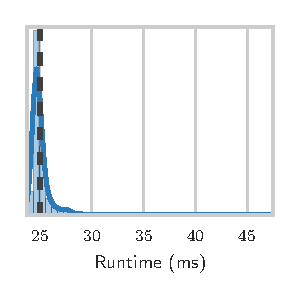
\includegraphics[width=\textwidth]{img/runtimes_histogram_1}
\vspace{-1.5em} % Shrink vertical padding
\caption{}
\label{fig:runtimes-histogram-1}
\end{subfigure}
~%
\begin{subfigure}[h]{.32\columnwidth}
\centering
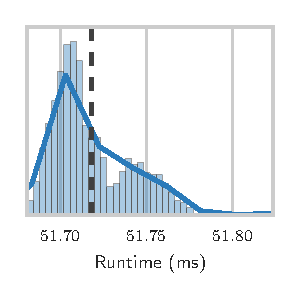
\includegraphics[width=\textwidth]{img/runtimes_histogram_2}
\vspace{-1.5em} % Shrink vertical padding
\caption{}
\label{fig:runtimes-histogram-2}
\end{subfigure}
~%
\begin{subfigure}[h]{.32\columnwidth}
\centering
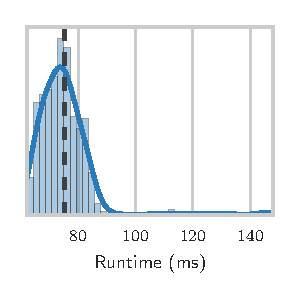
\includegraphics[width=\textwidth]{img/runtimes_histogram_3}
\vspace{-1.5em} % Shrink vertical padding
\caption{}
\label{fig:runtimes-histogram-3}
\end{subfigure}
\\
\begin{subfigure}[h]{.32\columnwidth}
\centering
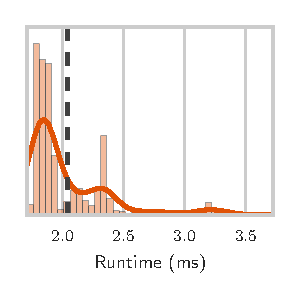
\includegraphics[width=\textwidth]{img/runtimes_histogram_4}
\vspace{-1.5em} % Shrink vertical padding
\caption{}
\label{fig:runtimes-histogram-4}
\end{subfigure}
~%
\begin{subfigure}[h]{.32\columnwidth}
\centering
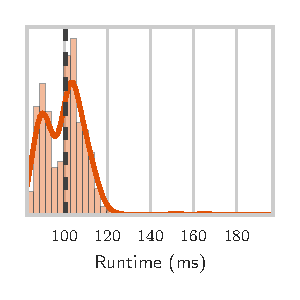
\includegraphics[width=\textwidth]{img/runtimes_histogram_5}
\vspace{-1.5em} % Shrink vertical padding
\caption{}
\label{fig:runtimes-histogram-5}
\end{subfigure}
~%
\begin{subfigure}[h]{.32\columnwidth}
\centering
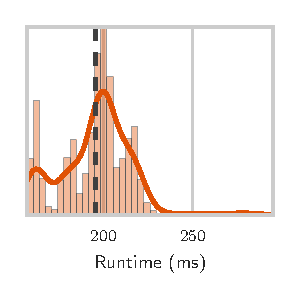
\includegraphics[width=\textwidth]{img/runtimes_histogram_6}
\vspace{-1.5em} % Shrink vertical padding
\caption{}
\label{fig:runtimes-histogram-6}
\end{subfigure}
\\
\begin{subfigure}[h]{.32\columnwidth}
\centering
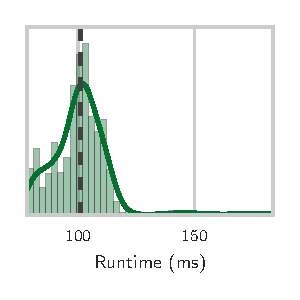
\includegraphics[width=\textwidth]{img/runtimes_histogram_7}
\vspace{-1.5em} % Shrink vertical padding
\caption{}
\label{fig:runtimes-histogram-7}
\end{subfigure}
~%
\begin{subfigure}[h]{.32\columnwidth}
\centering
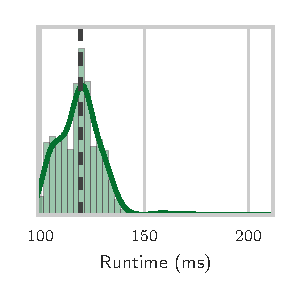
\includegraphics[width=\textwidth]{img/runtimes_histogram_8}
\vspace{-1.5em} % Shrink vertical padding
\caption{}
\label{fig:runtimes-histogram-8}
\end{subfigure}
~%
\begin{subfigure}[h]{.32\columnwidth}
\centering
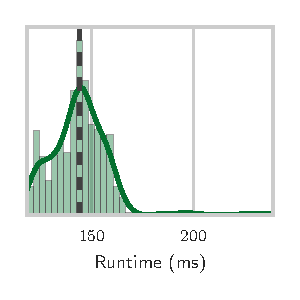
\includegraphics[width=\textwidth]{img/runtimes_histogram_9}
\vspace{-1.5em} % Shrink vertical padding
\caption{}
\label{fig:runtimes-histogram-9}
\end{subfigure}
\caption[Distribution of stencil code runtimes]{%
  Distribution of runtime samples for test cases from three
  devices. Each plot contains a 35-bin histogram of 1000 samples, and
  a fitted kernel density estimate with bandwidth 0.3. The sample mean
  is shown as a vertical dashed line. The top row are from the Intel
  i5-4570, the second row from the Nvidia GTX 590, and the third row
  from the AMD Tahiti 7970. In some of the plots, the distribution of
  runtimes is bimodal, and skewed to the lower end of the runtimes
  range.%
}
\label{fig:runtime-histograms}
\end{figure}

The complex interaction between processes competing for the finite
resources of a system introduces many sources for noise in program
runtime measurements. Before making any judgements about the relative
performance of optimisation configurations, we must establish the
level of noise present in these measurements. To do this, we evaluate
the distribution of runtimes for a randomly selected 1000 test cases,
recording 1000 runtime observations for each. We can then produce
fine-grained histograms of runtimes for individual test
cases. Figure~\ref{fig:runtime-histograms} shows an example nine of
these, for test cases from three devices. The plots show that the
distribution of runtimes is not always Gaussian; rather, it is
sometimes bimodal, and generally skewed to the lower end of the
runtime range, with a long ``tail'' to the right. This fits our
intuition that programs have a hard \emph{minimum} runtime enforced by
the time taken to execute the instructions of a program, and that
noise introduced to the system extends this runtime. For example,
preempting an OpenCL process on a CPU so that another process may run
may cause the very long tail visible in
Figure~\ref{fig:runtimes-histogram-1}.

The central limit theorem allows the assumption of an underlying
Gaussian distribution for samples of size $\ge 30$~\cite{Georges2007}.
Given our minimum sample size of 33, we can use 95\% confidence
intervals to provide statistical confidence that the arithmetic mean
of observed runtimes with respect to the true mean. As the number or
samples increases, we should expect the size of the confidence
interval to shrink. This is illustrated in Figure~\ref{fig:ci-trends},
which plots the average size of 95\% confidence intervals across the
1000 test cases, normalised to their respective means, as a function
of sample size. It shows the diminishing returns that increasing
sample size provides. For example, increasing the sample count from 10
to 30 results in an approximate 50\% reduction in confidence interval
size. Increasing the sample size from 30 to 50 results in only a 25\%
reduction.

\begin{figure}
\centering
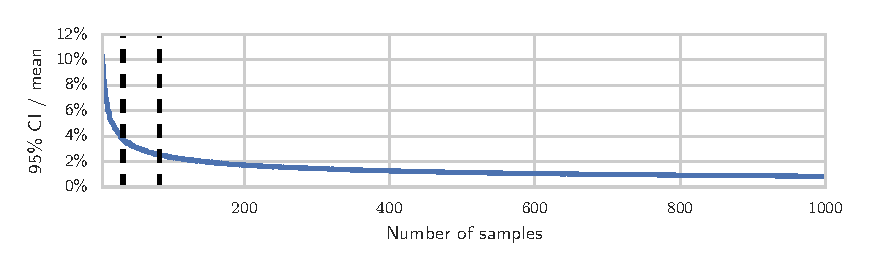
\includegraphics[width=\columnwidth]{img/ci_trend}
\caption[Confidence interval size vs.\ sample count]{%
  Ratio of confidence interval to mean as a function of sample
  count. Two dashed lines indicate the confidence intervals at the
  minimum (3.7\%) and mean (2.5\%) number of samples used in the
  experimental dataset.%
}
\label{fig:ci-trends}
\end{figure}

By comparing the average confidence interval at different sample
counts against the full experiment results of 269813 test cases, we
can assert with 95\% confidence that the true mean for each test case
is within 2.5\% of the sample mean (given the average number of
samples per test case), or 3.7\% in the worst case (at the minimum
number of samples). Since the differences between baseline and optimal
workgroup sizes is often well in excess of 100\%, there is no overlap
of confidence intervals between competing workgroup sizes.
% \FIXME{This demonstrates a sufficiently low level of noise that
% meaningful comparisons can be made between the performance of
% different configurations.}


\subsection{Workgroup Size Optimisation Space}

In this subsection we explore the impact that the workgroup size
optimisation space has on the performance of stencil codes.

\subsubsection{Oracle Workgroup Sizes}

\begin{figure}
\centering
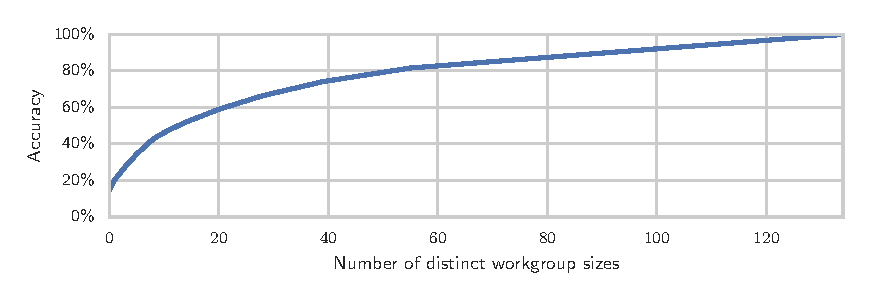
\includegraphics[width=\columnwidth]{img/num_params_oracle.pdf}
\caption[Oracle accuracy vs.\ number of workgroup sizes]{%
  Accuracy compared to the oracle as a function of the number of
  workgroup sizes used. The best accuracy that can be achieved using a
  single statically chosen workgroup size is 15\%. Achieving 50\%
  oracle accuracy requires a minimum of 14 distinct workgroup sizes.%
}
\label{fig:oracle-accuracy}
\end{figure}

For each scenario $s$, the oracle workgroup size $\Omega(s)$ is the
workgroup size which resulted in the lowest mean runtime. If the
performance of stencils were independent of workgroup size, we would
expect that the oracle workgroup size would remain constant across all
scenarios $s \in S$. Instead, we find that there are 135 unique oracle
workgroup sizes, with 31.5\% of scenarios having a unique workgroup
size. This demonstrates the difficult in attempting to tune for
\emph{optimal} parameter values, since 14 distinct workgroup sizes are
needed to achieve just 50\% of the oracle accuracy
(Figure~\ref{fig:oracle-accuracy}), although it is important to make
the distinction that oracle \emph{accuracy} and \emph{performance} are
not equivalent.

Figure~\ref{fig:oracle-wgsizes} shows the distribution of oracle
workgroup sizes, demonstrating that there is clearly no ``silver
bullet'' workgroup size which is optimal for all scenarios, and that
the space of oracle workgroup sizes is non linear and complex. The
workgroup size which is most frequently optimal is
$w_{(64 \times 4)}$, which is optimal for 15\% of scenarios. Note that
this is not adequate to use as a baseline for static tuning, as it
does not respect legality constraints, that is
$w_{(64 \times 4)} \not\in W_{safe}$.


\subsubsection{Workgroup Size Legality}

\begin{figure}
\begin{subfigure}[t]{0.98\columnwidth}
\centering
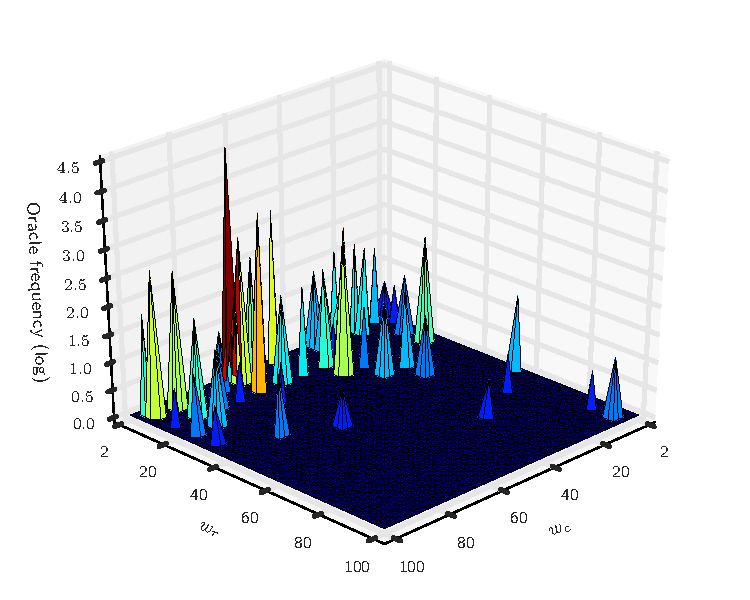
\includegraphics[width=\columnwidth]{img/oracle_param_space.pdf}
\vspace{-1.5em} % Shrink vertical padding
\caption{}
\label{fig:oracle-wgsizes}
\end{subfigure}
\\
\begin{subfigure}[t]{0.98\columnwidth}
\centering
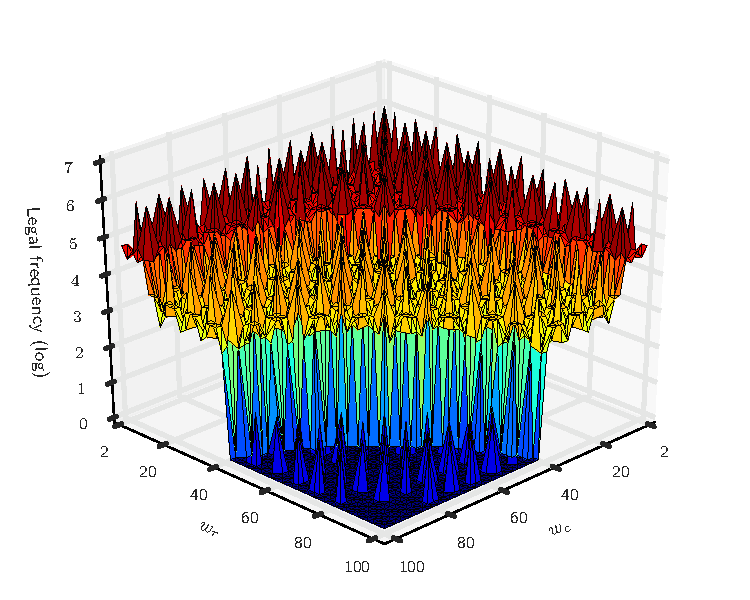
\includegraphics[width=\columnwidth]{img/coverage_space.pdf}
\vspace{-1.5em} % Shrink vertical padding
\caption{}
\label{fig:coverage}
\end{subfigure}
\caption[Workgroup size legality and optimality]{%
  Log frequency counts for: (\subref{fig:oracle-wgsizes}) optimality,
  and (\subref{fig:coverage}) legality for a subset of the aggregated
  workgroup size optimisation space, $w_c \le 100, w_r \le 100$. The
  space of oracle workgroup size frequencies is highly irregular and
  uneven, with a peak frequency of $w_{(64 \times 4)}$. Legality
  frequencies are highest for smaller row and column counts (where
  $w < W_{\max}(s) \forall s \in S$), and $w_c$ and $w_r$ values which
  are multiples of 8.%
}
\label{fig:heatmaps}
\end{figure}

As explained in Subsection~\ref{subsec:op-params}, the space of legal
workgroup sizes $W_{legal}(s)$ for a given scenario $s$ comprises all
workgroup sizes which: do not exceed the maximum allowed by the OpenCL
device and kernel $W_{\max}(s)$, and are not refused by the OpenCL
runtime.

\paragraph{Maximum workgroup sizes}

\begin{figure}
  \centering
  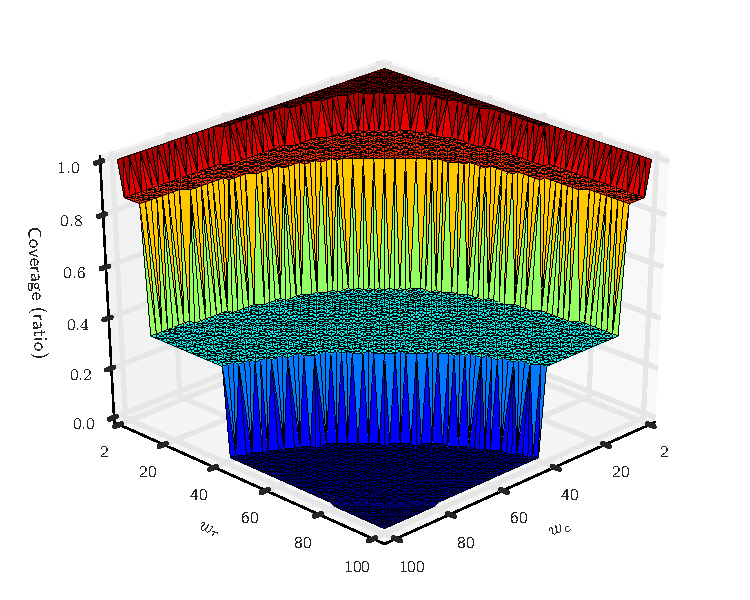
\includegraphics[width=\columnwidth]{img/max_wgsizes.pdf}
  \vspace{-1.5em} % Shrink vertical padding
  \caption[Workgroup size coverage]{%
    A subset of the aggregated workgroup size optimisation space,
    $w_c \le 100, w_r \le 100$, showing the \emph{coverage} of each
    workgroup size, i.e.\ the ratio of scenarios for which a workgroup
    size satisfies architecture and kernel enforced constraints
    ($W_{\max}(s)$). Workgroup sizes with a coverage of $< 1$ fail to
    satisfy these constraints for one or more scenarios. Only
    workgroup sizes with a coverage of 1 may be used for static
    tuning, which greatly reduces the size of the optimisation
    space. Observed $W_{\max}(s)$ values are multiples of 256, hence
    the abrupt ``steps'' in coverage.%
  }
\label{fig:max-wgsizes}
\end{figure}

We define the \emph{coverage} of a workgroup size to be the ratio
$0 \le x \le 1$ between the number of scenarios for which the
workgroup size was less than $W_{\max}(s)$, normalised to the total
number of workgroup sizes. A coverage of 1 implies a workgroup size
which is always legal for all combinations of stencil and
architecture. A workgroup size with a coverage of 0 is never
legal. Figure~\ref{fig:max-wgsizes} plots the coverage of a subset of
the workgroup size optimisation space.

Note that since $W_{\max}(s)$ defines a hard limit for a given $s$, if
statically selecting a workgroup size, one must limit the optimisation
space to the smallest $W_{\max}(s)$ value, i.e.\ only the workgroup
sizes with a coverage of 1. The observed $W_{\max}(s)$ values range
from 256--8192, which results in up to a 97\% reduction in the size of
the optimisation space when $W_{\max}(s) = 8192$, even though only
14\% of scenarios have the minimum value of $W_{\max}(s) = 256$.

% Size of optimisation space for Wmax =  256: 273
% Size of optimisation space for Wmax = 8192: 15925

\paragraph{Refused Parameters}

\begin{table}
\parbox{.45\linewidth}{
  \centering
  \scriptsize
  \begin{tabular}{lr}
    \toprule
    Parameter &  Refused (\%) \\
    \midrule
    $18 \times 24$ &          0.32 \\
    $26 \times 16$ &          0.31 \\
    $28 \times 32$ &          0.31 \\
    $4 \times 2$ &          0.31 \\
    $16 \times 14$ &          0.30 \\
    $14 \times 40$ &          0.30 \\
    $24 \times 36$ &          0.30 \\
    $36 \times 24$ &          0.30 \\
    $4 \times 26$ &          0.30 \\
    $4 \times 6$ &          0.30 \\
    \bottomrule
  \end{tabular}
}
\hfill
\parbox{.45\linewidth}{
  \centering
  \scriptsize
  \begin{tabular}{lr}
    \toprule
    Parameter &  Refused (\%) \\
    \midrule
    $8 \times 18$ &          0.30 \\
    $8 \times 22$ &          0.30 \\
    $14 \times 48$ &          0.29 \\
    $28 \times 24$ &          0.29 \\
    $30 \times 8$ &          0.29 \\
    $48 \times 14$ &          0.29 \\
    $8 \times 10$ &          0.29 \\
    $10 \times 8$ &          0.28 \\
    $24 \times 18$ &          0.28 \\
    $26 \times 32$ &          0.28 \\
    \bottomrule
  \end{tabular}
}
\caption[Workgroup sizes most frequently refused]{%
  The twenty most refused parameters, ranked in descending
  order. There is little correlation between the size of workgroup and the
  likelihood that it is refused, suggesting that the cause of refused
  parameters is not a resource constraint, but a behavioural issue.%
}
\label{tab:top-refused-params}
\end{table}

\begin{figure*}
  \centering
  \begin{subfigure}[h]{.45\textwidth}
    \centering
    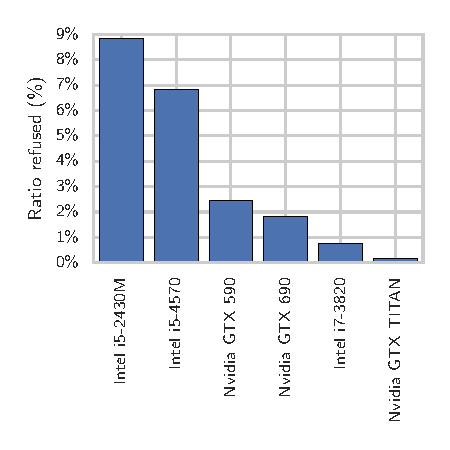
\includegraphics[width=.8\textwidth]{img/refused_params_by_device}
    \caption{}
    \label{fig:refused-params-by-device}
  \end{subfigure}
  ~%
  \begin{subfigure}[h]{.45\textwidth}
    \centering
    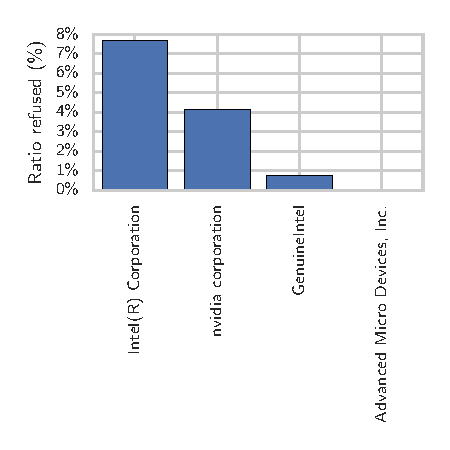
\includegraphics[width=.8\textwidth]{img/refused_params_by_vendor}
    \caption{}
    \label{fig:refused-params-by-vendor}
  \end{subfigure}
  \caption[Refused workgroup sizes by device and vendor]{%
    The ratio of test cases with refused workgroup sizes, grouped by:
    (\subref{fig:refused-params-by-device}) OpenCL device ID;\
    (\subref{fig:refused-params-by-vendor}) device vendor ID. Parameters
    were refused most frequently by Intel i5 CPUs, then by
    previous-generation NVIDIA GPUs. No parameters were refused by AMD
    devices.%
  }
  \label{fig:refused-params-by-dev-vendor}
\end{figure*}

In addition to the hard constraints imposed by the maximum workgroup
size, there are also refused parameters, which are workgroup sizes
which are rejected by the OpenCL runtime and do not provide a
functioning program. Of the 8504 unique workgroup sizes tested, 11.4\%
were refused in one or more test cases. An average of 5.5\% of all
test cases lead to refused parameters. For a workgroup size to be
refused, it must satisfy the architectural and program-specific
constraints which are exposed by OpenCL, but still lead to a
\texttt{CL\_OUT\_OF\_RESOURCES} error when the kernel is
enqueued. Table~\ref{tab:top-refused-params} lists the most frequently
refused parameters, and the percentage of test cases for which they
were refused. While uncommon, a refused parameter is an obvious
inconvenience to the user, as one would expect that any workgroup size
within the specified maximum should behave \emph{correctly}, if not
efficiently. Figure~\ref{fig:coverage} visualises the space of legal
workgroup sizes by showing the frequency counts that a workgroup size
is legal. Smaller workgroup sizes are legal most frequently due to the
$W_{\max}(s)$ constraints. Beyond that, workgroup sizes which contain
$w_c$ and $w_r$ values which are multiples of eight are more
frequently legal, which is a common width of SIMD vector
operations~\cite{IntelCorporation2012}.

Experimental results suggest that the problem is vendor --- or at
least device --- specific. By grouping the refused test cases by
device and vendor, we see a much greater quantity of refused
parameters for test cases on Intel CPU devices than any other type,
while no workgroup sizes were refused by the AMD
GPU. Figure~\ref{fig:refused-params-by-dev-vendor} shows these
groupings. The exact underlying cause for these refused parameters is
unknown, but can likely by explained by inconsistencies or errors in
specific OpenCL driver implementations.

As these OpenCL implementations are still in active development, it is
anticipated that errors caused by unexpected behaviour will become
more infrequent as the technology
matures. Figure~\ref{fig:refused-params-by-device} shows that the
ratio of refused parameters decreases across the three generations of
Nvidia GPUs: GTX 590 (2011), GTX 690 (2012), and GTX TITAN (2013). The
same trend is apparent for the two Intel i5s: i5-2430M (2011), and
i5-4570 (2013), although not for the i7-3820 (2012). For now, it is
imperative that any autotuning system is capable of adapting to these
refused parameters by suggesting alternatives when they occur.


\subsubsection{Baseline Parameter}

The baseline parameter $\bar{w}$ is the workgroup size which provides
the best overall performance while being legal for all scenarios. It
is the workgroup size $w \in W_{safe}$ which maximises the output of
the performance function $\bar{p}(w)$. As shown in
Table~\ref{tab:highest-legality}, only a \emph{single} workgroup size
$w_{(4 \times 4)}$ from the set of experimental results is found to
have a legality of 100\%, suggesting that an adaptive approach to
setting workgroup size is necessary not just for the sake of
maximising performance, but also for guaranteeing program correctness.

The utility of the baseline parameter is that it represents the best
performance that can be achieved through static tuning of the
workgroup size parameter. We can evaluate the performance of
suboptimal workgroup sizes by calculating the geometric mean of their
\emph{performance} for a particular scenario $p(s, w)$ across all
scenarios, $\bar{p}(w)$. The baseline parameter $\bar{p}(\bar{w})$
achieves only 24\% of the available
performance. Figure~\ref{fig:performance-legality} plots workgroup
size \emph{legality} and \emph{performance}, showing that there is no
clear correlation between the two. In fact, the workgroup sizes with
the highest mean performance are valid only for scenarios with the
largest $W_{\max}(s)$ value, which account for less than 1\% of all
scenarios, further reinforcing the case for adaptive tuning. The
workgroup sizes with the highest legality are listed in
Table~\ref{tab:highest-legality}, and the workgroup sizes with the
highest performance are listed in Table~\ref{tab:highest-performance}.

Figure~\ref{fig:speedups} shows the speedup of the oracle workgroup
size over the baseline parameter $w_{(4 \times 4)}$ for all
scenarios. If we assume that sufficiently pragmatic developer with
enough time would eventually find this static optimal, then this
provides a reasonable comparison for calculating speedups of an
autotuner for workgroup size. Comparing the runtime of workgroup sizes
relative to the oracle allows us to calculate upper bounds on the
possible performance which can be expected from autotuning.


\begin{figure}
\centering
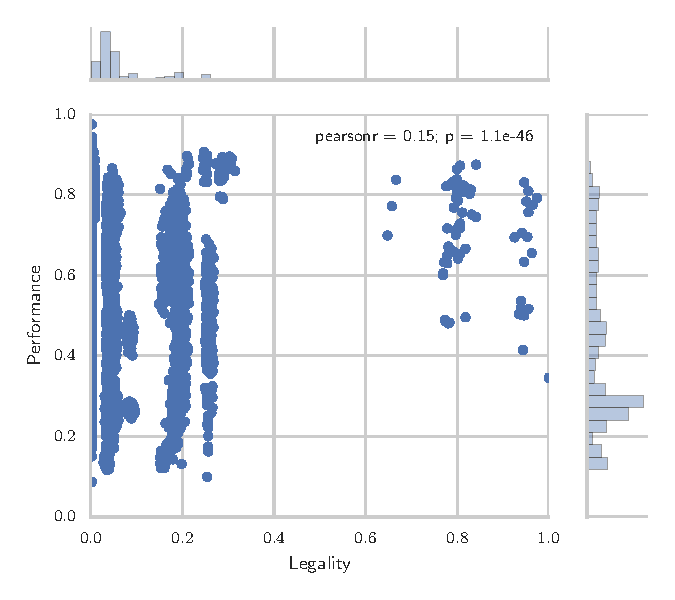
\includegraphics[width=\columnwidth]{img/params_summary.pdf}
\caption[Workgroup size legality vs.\ performance]{%
  Average legality and performance relative to the oracle of all
  workgroup sizes. Clearly, the relationship between legality and
  performance is not linear. Distinct vertical ``bands'' appear
  between regions of legality caused by the different $W_{\max}(s)$
  values of devices. The irregular jitter between these vertical bands
  is caused by refused parameters.%
}
\label{fig:performance-legality}
\end{figure}


\begin{table}
  \centering
  \scriptsize
  \begin{tabular}{lrr}
    \toprule
    Parameter &  Legality (\%) &  Performance (\%) \\
    \midrule
    $4 \times 4$ &          100.0 &              34.6 \\
    $32 \times 4$ &           97.4 &              79.2 \\
    $40 \times 4$ &           96.5 &              77.5 \\
    $16 \times 4$ &           96.3 &              65.5 \\
    $56 \times 4$ &           95.6 &              81.0 \\
    $16 \times 8$ &           95.6 &              75.7 \\
    $8 \times 4$ &           95.6 &              51.7 \\
    $24 \times 4$ &           95.3 &              69.6 \\
    $24 \times 8$ &           95.1 &              78.4 \\
    $48 \times 4$ &           94.6 &              83.1 \\
    $8 \times 8$ &           94.6 &              63.4 \\
    $4 \times 16$ &           94.6 &              50.1 \\
    $4 \times 8$ &           94.4 &              41.5 \\
    $8 \times 16$ &           94.2 &              70.6 \\
    $4 \times 40$ &           94.2 &              50.2 \\
    $4 \times 32$ &           93.9 &              53.6 \\
    $4 \times 48$ &           93.9 &              51.9 \\
    $4 \times 56$ &           93.9 &              50.3 \\
    $4 \times 24$ &           93.5 &              50.4 \\
    $8 \times 24$ &           92.5 &              69.5 \\
    $64 \times 4$ &           84.1 &              87.5 \\
    $16 \times 16$ &           84.1 &              74.5 \\
    $24 \times 16$ &           83.2 &              75.1 \\
    $32 \times 8$ &           83.0 &              81.3 \\
    $40 \times 16$ &           82.8 &              80.3 \\
    \bottomrule
  \end{tabular}
  \caption[Workgroup sizes with greatest legality]{%
    The 25 workgroup sizes with the greatest legality.%
  }
  \label{tab:highest-legality}
\end{table}

\begin{table}
  \centering
  \scriptsize
  \begin{tabular}{lrr}
    \toprule
    Parameter &  Legality (\%) &  Performance (\%) \\
    \midrule
    $270 \times 24$ &            0.2 &              97.5 \\
    $174 \times 38$ &            0.2 &              94.4 \\
    $310 \times 20$ &            0.2 &              94.2 \\
    $546 \times 10$ &            0.2 &              93.0 \\
    $282 \times 16$ &            0.2 &              93.0 \\
    $520 \times 10$ &            0.2 &              92.9 \\
    $520 \times 12$ &            0.2 &              92.3 \\
    $746 \times 8$ &            0.2 &              92.0 \\
    $38 \times 140$ &            0.2 &              91.9 \\
    $300 \times 18$ &            0.2 &              91.3 \\
    $700 \times 6$ &            0.2 &              91.1 \\
    $96 \times 24$ &           24.7 &              90.6 \\
    $88 \times 48$ &            0.7 &              90.6 \\
    $820 \times 6$ &            0.2 &              90.4 \\
    $88 \times 32$ &           24.9 &              90.0 \\
    $96 \times 32$ &           25.4 &              89.8 \\
    $88 \times 40$ &           21.0 &              89.7 \\
    $80 \times 16$ &           30.3 &              89.6 \\
    $722 \times 10$ &            0.2 &              89.5 \\
    $280 \times 24$ &            0.2 &              89.5 \\
    $910 \times 6$ &            0.2 &              89.4 \\
    $88 \times 24$ &           28.7 &              89.4 \\
    $64 \times 24$ &           29.4 &              89.2 \\
    $80 \times 32$ &           24.5 &              89.2 \\
    $72 \times 16$ &           29.4 &              89.2 \\
    \bottomrule
  \end{tabular}
  \caption[Workgroup sizes with greatest performance]{%
    The 25 workgroup sizes with the greatest mean
    performance.%
  }
  \label{tab:highest-performance}
\end{table}


\subsubsection{Speedup Upper Bounds}

\begin{figure}
  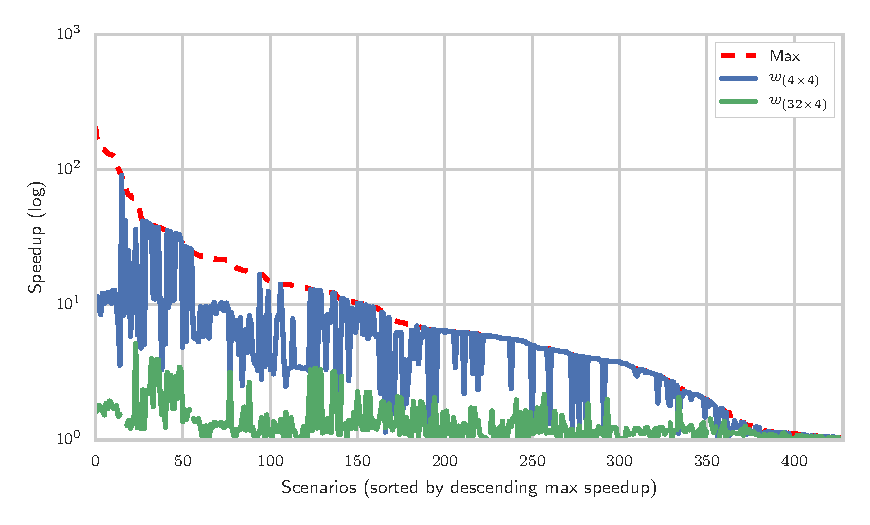
\includegraphics[width=\columnwidth]{img/max_speedups}
  \caption[Workgroup size speedups]{%
    Speedup of oracle workgroup size over: the worst performing
    workgroup size for each scenario (\emph{Max}), the statically
    chosen workgroup size that provides the best overall performance
    ($w_{(4 \times 4)}$), and the human expert selected parameter
    ($w_{(32 \times 4)}$). Note that the human expert parameter is not
    legal for all scenarios.%
  }
\label{fig:speedups}
\end{figure}

For a given scenario $s$, the ratio of the workgroups sizes from
$W_{legal}(s)$ which provide the longest and shortest mean runtimes is
used to calculate an upper bound for the possible performance
influence of workgroup size:
%
\begin{equation}
r_{max}(s) = r(s, \argmax_{w \in W_{legal}(s)} t(s,w), \Omega(s))
\end{equation}
%
When applied to each scenario $s \in S$ of the experimental results,
we find the average of speedup upper bounds to be $15.14\times$ (min
$1.03\times$, max $207.72\times$). This demonstrates the importance of
tuning stencil workgroup sizes --- if chosen incorrectly, the runtime
of stencil programs can be extended by up to $207.72\times$. Note too
that for 5 of the scenarios, the speedup of the best over worst
workgroup sizes is $\le 5\%$.
% TODO: t-test for this!
For these scenarios, there is little benefit to autotuning; however,
this represents only 1.1\% of the tested scenarios. For 50\% of the
scenarios, the speedup of the best over worst workgroup sizes is
$\ge 6.19\times$.


\subsubsection{Human Expert}

% SCENARIOS IN WHICH 32x4 WAS NOT LEGAL:
%
% sqlite> select distinct name,kernels.north,kernels.south,kernels.east,kernels.west,device,dataset,name from runtime_stats left join scenarios on runtime_stats.scenario=scenarios.id left join kernel_names on scenarios.kernel=kernel_names.id left join kernels on scenarios.kernel=kernels.id where scenario NOT IN (select scenario from runtime_stats where params="32x4");
% name        north       south       east        west        device                                     dataset                name
% ----------  ----------  ----------  ----------  ----------  -----------------------------------------  ---------------------  ----------
% complex     30          30          30          30          1xIntel(R) Core(TM) i5-4570 CPU @ 3.20GHz  1024.1024.float.float  complex
% simple      0           0           0           0           1xIntel(R) Core(TM) i5-2430M CPU @ 2.40GH  1024.1024.float.float  simple
% complex     30          30          30          30          1xIntel(R) Core(TM) i5-2430M CPU @ 2.40GH  2048.2048.float.float  complex
% complex     1           10          30          30          1xIntel(R) Core(TM) i5-4570 CPU @ 3.20GHz  512.512.float.float    complex
% simple      30          30          30          30          1xIntel(R) Core(TM) i5-2430M CPU @ 2.40GH  512.512.float.float    simple
% complex     30          30          30          30          1xGeForce GTX 690                          512.512.float.float    complex
% simple      20          10          20          10          1xIntel(R) Core(TM) i5-2430M CPU @ 2.40GH  4096.4096.float.float  simple
% simple      1           10          30          30          1xIntel(R) Core(TM) i5-2430M CPU @ 2.40GH  2048.2048.float.float  simple
% complex     30          30          30          30          1xGeForce GTX 690                          1024.1024.float.float  complex
% complex     1           10          30          30          1xIntel(R) Core(TM) i5-2430M CPU @ 2.40GH  2048.2048.float.float  complex
% simple      30          30          30          30          1xGeForce GTX 690                          512.512.float.float    simple

In the original implementation of the SkelCL stencil
skeleton~\cite{Breuer2013}, \citeauthor{Breuer2013} selected a
workgroup size of $w_{(32 \times 4)}$ in an evaluation of 4 stencil
operations on a Tesla S1070 system. We can use this as an additional
parameter to compare the relative performance of workgroup sizes
against. However, the $w_{(32 \times 4)}$ workgroup size is invalid
for 2.6\% of scenarios, as it is refused in 11 test cases. By device,
those are: 3 on the GTX 690, 6 on the i5-2430M, and 2 on the i5-4570.
For the scenarios where $w_{(32 \times 4)}$ \emph{is} legal, the human
expert chosen workgroup size achieves an impressive geometric mean of
79.2\% of the oracle performance. The average speedup of oracle
workgroup sizes over the workgroup size selected by a human expert is
$1.37\times$ (min $1.0\times$, max $5.17\times$). Since the workgroup
size selected by the human expert is not legal for all scenarios, we
will examine the effectiveness of heuristics for tuning workgroup
size.


\subsubsection{Heuristics}

In this subsection we will consider the effectiveness of instead
selecting workgroup size using two types of heuristics. The first,
using the maximum workgroup size returned by the OpenCL device and
kernel APIs to select the workgroup size adaptively. The second, using
per-device heuristics, in which the workgroup size is selected based
on the specific architecture that a stencil is operating on.

\paragraph{Using maximum legal size}

A common approach taken by OpenCL developers is to set the workgroup
size for a kernel based on the maximum legal workgroup size queried
from the OpenCL APIs. For example, to set the size of 2D workgroup, a
developer the square root of the (scalar) maximum wgsize to set the
number of columns and rows (since $w_c \cdot w_r$ must be
$< W_{\max}(s)$). To consider the effectiveness of this approach, we
group the workgroup size performances based on the ratio of the
maximum allowed for each scenario. We can also perform this for each
of the two dimensions --- rows and columns --- of the stencil
workgroup size.

Figure~\ref{fig:performance-wgsizes} shows the distribution of
runtimes when grouped this way, demonstrating that the performance of
(legal) workgroup sizes are not correlated with the maximum workgroup
sizes $W_{\max}(s)$. However, when considering individual components,
we observe that the best median workgroup size performances are
achieved with a number of columns that is between 10\% and 20\% of the
maximum, and a number of rows that is between 0\% and 10\% of the
maximum.

\paragraph{Per-device workgroup sizes}

\begin{table}
  \scriptsize
  \centering
  \begin{tabular}{lllp{1cm}p{1cm}}
    \toprule
    Device &         Oracle & Legality & Perf.\ min & Perf.\ avg. \\
    \midrule
    AMD Tahiti 7970 &   $48\times 4$ &      1.0 &       0.54 &        0.91 \\
    Intel i5-2430M &  $64\times 16$ &      0.8 &       0.37 &        0.91 \\
    Intel i5-4570 &   $88\times 8$ &     0.89 &       0.33 &        0.89 \\
    Intel i7-3820 &  $40\times 24$ &     0.95 &       0.76 &        0.97 \\
    NVIDIA GTX 590 &  $12\times 2$ &      0.8 &        0.2 &         0.9 \\
    NVIDIA GTX 690 &   $64\times 4$ &     0.93 &       0.32 &        0.84 \\
    NVIDIA GTX TITAN &   $64\times 4$ &      1.0 &       0.26 &        0.81 \\
    \textbf{CPUs} &   $88\times 8$ &     0.88 &       0.33 &        0.91 \\
    \textbf{GPUs} &   $64\times 4$ &     0.76 &       0.26 &        0.86 \\
    \bottomrule
  \end{tabular}
  \caption[Performance of tuning with a per-device heuristic]{%
    Selecting workgroup size using a per-device heuristic. The mode
    optimal workgroup size for each device type $\bar{w}$ is evaluated
    based on legality, and relative performance to the oracle (minimum
    and average) when legal.%
  }
  \label{tab:heuristic-dev}
\end{table}

One possible technique to selecting workgroup size is to tune
particular values for each targeted execution device. This approach is
sometimes adopted for cases with particularly high requirements for
performance on a single platform, so it produces an interesting
contrast to evaluating a machine learning approach, which attempts to
predict workgroup sizes for unseen platforms without the need for an
expensive exploration phase on the new platform.

Figure~\ref{fig:performances} shows the performance of workgroup sizes
relative to the oracle across scenarios grouped by: kernel, device,
and dataset. When grouped like this, a number of observations can
made. First is that not all of the kernels are sensitive to tuning
workgroup size to the same degree. The \emph{sobel} kernel has the
lowest median performance, indicating that it is the most profitable
to tune, while the \emph{threshold} kernel is the least
profitable. Similarly, the Intel i7-3820 is far less amenable to
tuning than the other devices, while the Intel i5-4570 is the most
sensitive to the workgroup size parameter. Such variances in the
distributions of workgroup sizes suggest that properties underlying
the architecture, kernel, and dataset all contribute towards the
proper selection of workgroup size.

To test the performance of a per-device heuristic for selecting
workgroup size, we group the scenarios by device, and compare the
relative performance of all workgroup sizes for each group of
scenarios. The most frequently optimal workgroup size $\bar{w}$ for
each device is selected, and the legality and performance of each
scenario using that workgroup size is evaluated.
Table~\ref{tab:heuristic-dev} shows the results of this evaluation.
The GTX 690 and GTX TITAN share the same $\bar{w}_{(64 \times 4)}$
value, while every other device has a unique optimum. The general case
performance of these per-device parameters is very good, although
legality is only assured for the GTX TITAN and AMD 7970 (which did not
refuse any parameters). However, the worst case performance of
per-device workgroup sizes is poor for all except the i7-3820 (which
is least sensitive to tuning), suggesting that device alone is not
capable of reliably informing the choice of workgroup size.


\begin{figure}
  \begin{subfigure}[h]{\columnwidth}
    \centering
    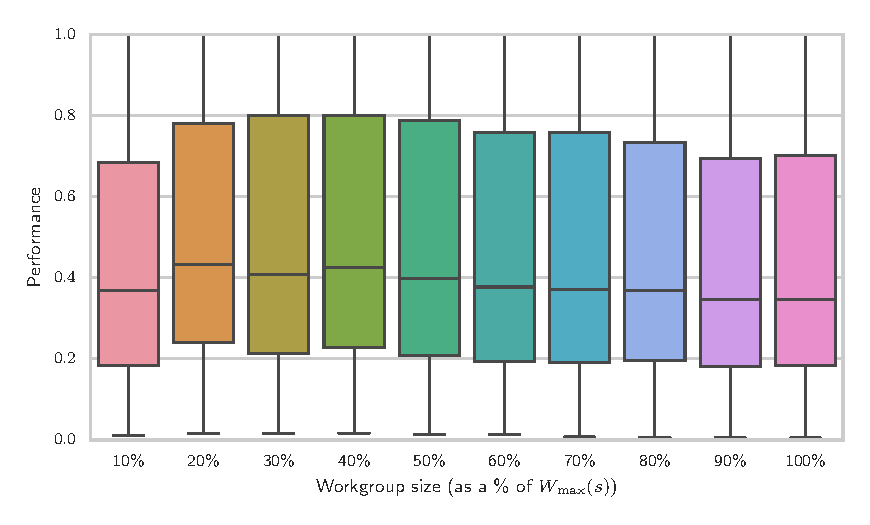
\includegraphics[width=\columnwidth]{img/performance_max_wgsize}
    \vspace{-1.5em} % Shrink vertical padding
    \caption{}
    \label{fig:performance-max-wgsize}
  \end{subfigure}
  \\
  \begin{subfigure}[h]{.48\columnwidth}
    \centering
    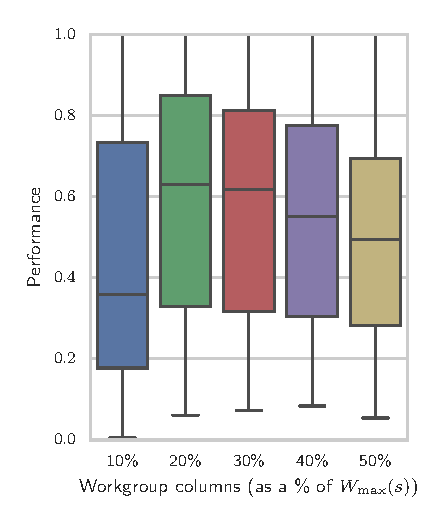
\includegraphics[width=\columnwidth]{img/performance_max_c}
    \vspace{-1.5em} % Shrink vertical padding
    \caption{}
    \label{fig:performance-wg-c}
  \end{subfigure}
  ~%
  \begin{subfigure}[h]{.48\columnwidth}
    \centering
    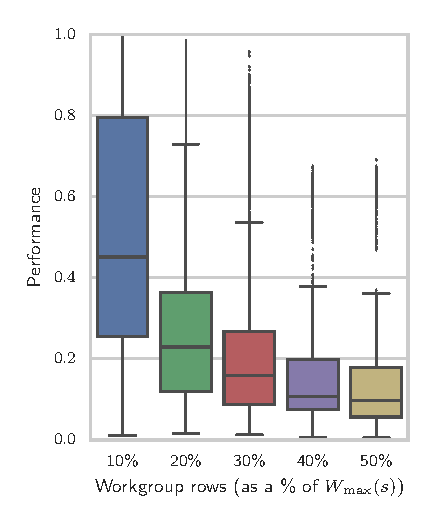
\includegraphics[width=\columnwidth]{img/performance_max_r}
    \vspace{-1.5em} % Shrink vertical padding
    \caption{}
    \label{fig:performance-wg-r}
  \end{subfigure}

  \caption[Workgroup size performances vs.\ size]{%
    Comparing workgroup performance relative to the oracle as function
    of: (\subref{fig:performance-max-wgsize})~maximum legal size,
    (\subref{fig:performance-wg-c})~number of columns, and
    (\subref{fig:performance-wg-r})~ number of rows. Each workgroup
    size is normalised to the maximum allowed for that scenario, $W_{\max}(s)$.%
  }
  \label{fig:performance-wgsizes}
\end{figure}

\begin{figure}
  \begin{subfigure}[h]{\columnwidth}
    \centering
    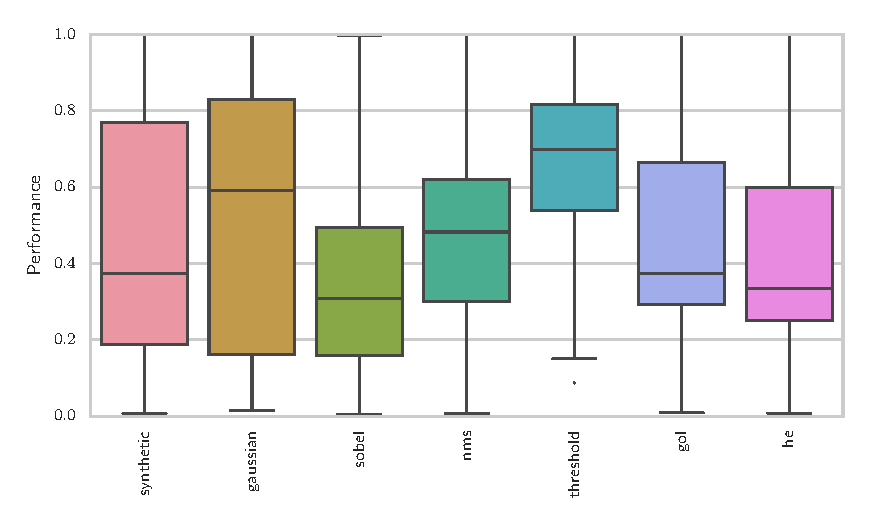
\includegraphics[width=\columnwidth]{img/performance_kernels.pdf}
    \vspace{-1.5em} % Shrink vertical padding
    \caption{}
    \label{fig:performance-kernels}
  \end{subfigure}
  \\
  \begin{subfigure}[h]{.48\columnwidth}
    \centering
    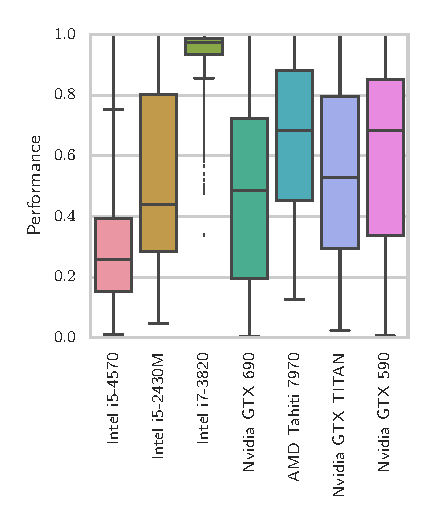
\includegraphics[width=\columnwidth]{img/performance_devices.pdf}
    \vspace{-1.5em} % Shrink vertical padding
    \caption{}
    \label{fig:performance-devices}
  \end{subfigure}
  ~%
  \begin{subfigure}[h]{.48\columnwidth}
    \centering
    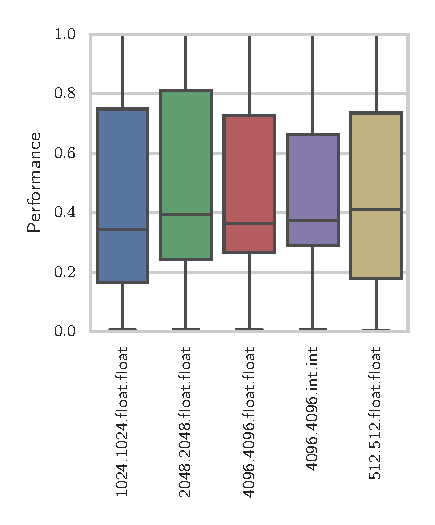
\includegraphics[width=\columnwidth]{img/performance_datasets.pdf}
    \vspace{-1.5em} % Shrink vertical padding
    \caption{}
    \label{fig:performance-datasets}
  \end{subfigure}
  \caption[Workgroup size performances across device, kernel, and dataset]{%
    Performance relative to the oracle of workgroup sizes across all
    test cases, grouped by: (\subref{fig:performance-kernels})~kernels,
    (\subref{fig:performance-devices})~devices, and
    (\subref{fig:performance-datasets})~datasets.%
  }
  \label{fig:performances}
\end{figure}


\subsubsection{Summary}

In this subsection we have explored the performance impact of the
workgroup size optimisation space. By comparing the relative
performance of an average of 629 workgroup sizes for each of 429
scenarios, the following conclusions can be drawn:

\begin{enumerate}
\item The performance of a workgroup size for a particular scenario
  depends properties of the hardware, software, and dataset.
\item The performance gap between the best and workgroup sizes for a
  particular combination of hardware, software, and dataset is up to
  $207.72\times$.
\item Not all workgroup sizes are legal, and the space of legal
  workgroup sizes cannot statically be determined. Adaptive tuning of
  workgroup size is required to ensure reliable performance.
\item Differing scenarios have wildly different optimal workgroup
  sizes, and the best performance can be achieved using static tuning
  is optimal for only 15\% of scenarios.
\end{enumerate}
%
% I believe this presents a compelling case for the development of an
% autotuner which can select the optimal workgroup size at runtime.
%
In the following subsection, we will evaluate the performance of OmniTune
for selecting workgroup sizes.


\subsection{Autotuning Workgroup Sizes}

In this subsection, we evaluate the performance of OmniTune for
predicting workgroup sizes of SkelCL skeletons using the prediction
techniques described in Subsection~\ref{subsec:omnitune-ml}. For each
technique, we partition the experimental data into training and
testing sets, $S_{training} \subset S$ and
$S_{testing} = S - S_{training}$. A set of labelled training data
$D_{training}$ is derived from $S_{training}$, and the prediction
quality is testing using the validation set $D_{testing}$ derived from
$S_{training}$. We use multiple approaches to partitioning test data
to evaluate the prediction quality under different scenarios. The
processes for generating validation sets are:
%
\begin{itemize}
\item 10-fold --- shuffle the set of all data and divide into 10
  validation sets, each containing 10\% of the data. This process is
  repeated for 10 rounds, resulting in 100 validations of 10
  permutations of the data.
\item Synthetic --- divide the training data such that it consists
  solely of data collected from synthetic benchmarks, and use data
  collected from real-world benchmarks to test.
\item Device --- partition the training data into $n$ sets, one for
  each device. Use $n-1$ sets for training, repeating until every
  partition has been used for testing once.
\item Kernel --- partition the training data into $n$ sets, one for
  each kernel. Use $n-1$ sets for training, repeating until every
  partition has been used for testing once.
\item Dataset --- partition the training data into $n$ sets, one for
  each type of dataset. Use $n-1$ sets for training, repeating until
  every partition has been used for testing once.
\end{itemize}
%
For each autotuning technique, the results of testing using the
different validation sets are reported separately. The autotuning
techniques evaluated are: using classifiers to predict the optimal
workgroup size of a stencil, with fallback strategies to handle
illegal predictions; using regressors to predict the runtime of a
stencil using different workgroup sizes, and selecting the legal
workgroup size which has the lowest predicted runtime; and using
regressors to predict the relative performance of workgroup sizes over
a baseline, and selecting the workgroup size which has the highest
predicted relative performance. We first describe the evaluation
strategies for each technique, before presenting experimental results
and analysis.


\subsubsection{Evaluating Classifiers}

Training data consists of pairs of feature vectors $f(s)$ and oracle
workgroup sizes $\Omega(s)$:
%
\begin{equation}
  D_{training} = \left\{ (f(s),\Omega(s)) | s \in S_{training} \right\}
\end{equation}
%
Testing data are not labelled with oracle workgroup sizes:
%
\begin{equation}
  D_{testing} = \left\{ f(s) | s \in S_{testing} \right\}
\end{equation}
%
Each classifier is evaluated using the three different classification
techniques: \textsc{Baseline}, \textsc{Random}, and
\textsc{NearestNeighbour}, which differ in the way in which they
handle illegal predictions. Illegal predictions occur either because
the classifier has suggested a parameter which does not satisfy the
maximum workgroup size constraints $w < W_{\max}(s)$, or because the
workgroup size is refused by OpenCL $w \in W_{refused}(s)$. Workgroup
sizes are predicted for each scenario in the testing set, and the
quality of the predicted workgroup size is evaluated using the
following metrics:
%
\begin{itemize}
\item accuracy (binary) --- whether the predicted workgroup size is
  the true oracle, $p(f(s)) = \Omega(s)$.
\item validity (binary) --- whether the classifier predicted a
  workgroup size which satisfies the workgroup size constraints
  constraints, $p(f(s)) < W_{\max}(s)$.
\item refused (binary) --- whether the classifier predicted a
  workgroup size which is refused, $p(f(s)) \in W_{refused}(s)$.
\item performance (real) --- the relative performance of the predicted
  workgroup size relative to the oracle,
  $0 \le r(p(f(s)), \Omega(s)) \le 1$.
\item speedups (real) --- the relative performance of the predicted
  workgroup size relative to the baseline workgroup size
  $w_{(4 \times 4)}$, and human expert workgroup size
  $w_{(32 \times 4)}$ (where applicable).
\item time (real) --- the round trip time required to make the prediction,
  as measured by the OmniTune client. This includes classification
  time and inter-process communication overheads between the client
  and server.
\end{itemize}
%
The \emph{validty} and \emph{refused} metrics measure how often
fallback strategies are required to select a legal workgroup size
$w \in W_{legal}(s)$.


\subsubsection{Evaluating Regressors}

The evaluation approach for predicting runtimes and speedups is the
same; only the training data differs. For predicting runtimes,
training data consists of feature vectors, labelled with the mean
observed runtime $t(s,w)$ for all legal workgroup sizes:
%
\begin{equation}
  D_{training} = \bigcup_{\forall s \in S_{training}} \left\{ (f(s),t(s,w)) | w \in W_{legal}(s)
  \right\}
\end{equation}
For predicting speedups, the features vectors are labelled with
observed speedup over the baseline parameter $\bar{w}$ for all legal
workgroup sizes:
\begin{equation}
\begin{split}
  D_{training} = \cup \left\{ (f(s),r(s,w,\bar{w})) | w \in W_{legal}(s)
  \right\} \forall \\
  s \in S_{training}
\end{split}
\end{equation}
%
Test data consists of unlabelled feature vectors:
%
\begin{equation}
  D_{testing} = \left\{ f(s) | s \in S_{testing} \right\}
\end{equation}
%
The quality of predicted workgroup sizes is evaluated using the
following metrics:
%
\begin{itemize}
\item accuracy (binary) --- whether the predicted workgroup size is
  the true oracle, $p(f(s)) = \Omega(s)$.
\item performance (real) --- the relative performance of the predicted
  workgroup size relative to the oracle,
  $0 \le r(p(f(s)), \Omega(s)) \le 1$.
\item speedups (real) --- the relative performance of the predicted
  workgroup size relative to the baseline workgroup size
  $w_{(4 \times 4)}$, and human expert workgroup size
  $w_{(32 \times 4)}$ (where applicable).
\item time (real) --- the round trip time required to make the
  prediction, as measured by the OmniTune client. This includes
  classification time and inter-process communication overheads
  between the client and server.
\end{itemize}
%
Unlike with classifiers, the process of selecting workgroup sizes
using regressors is resistant to refused parameters, so no fallback
strategies are required, and the \emph{validity} and \emph{refused}
metrics are not used.


\subsubsection{Results and Analysis}

The purpose of this evaluation is to test the effectiveness of machine
learning-enabled autotuning for predicting workgroup sizes of SkelCL
stencils codes. First, we consider the prediction performance of
classifiers.


\begin{figure}
\centering
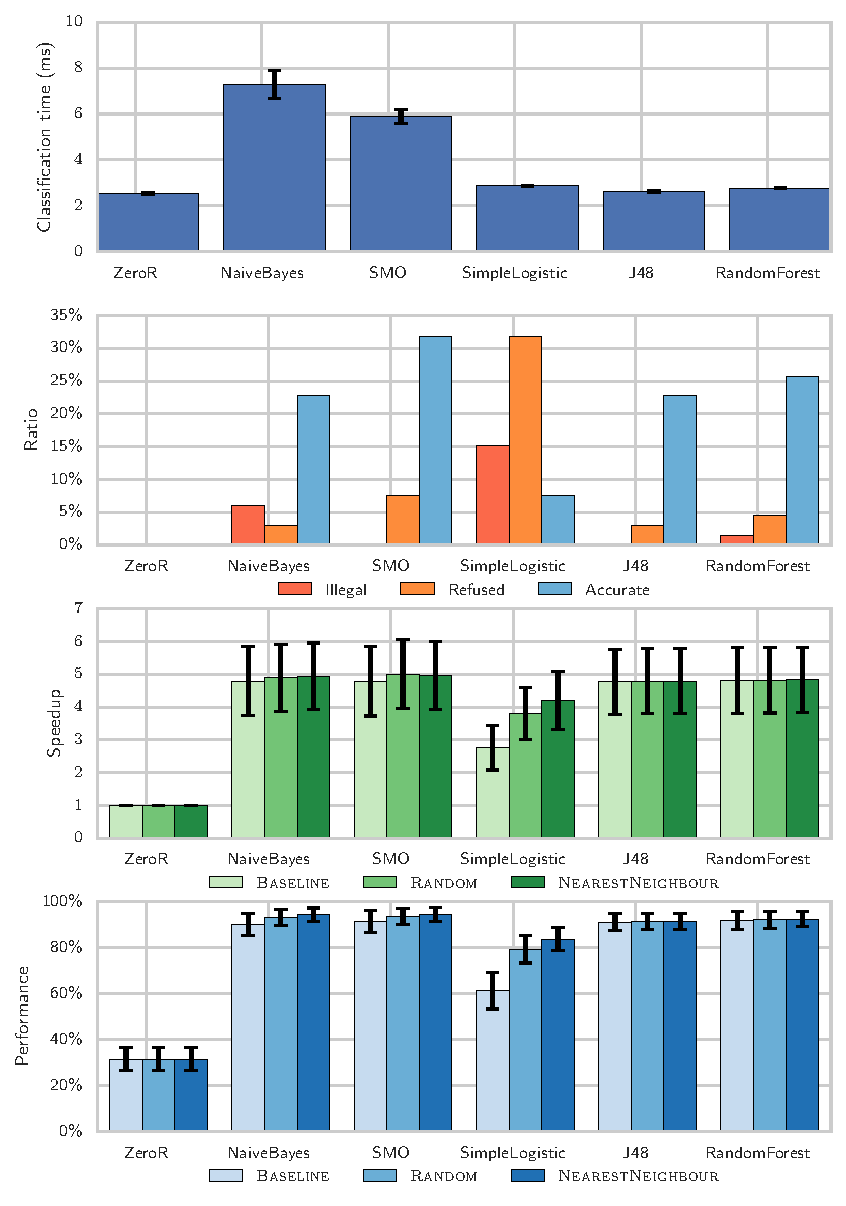
\includegraphics[width=\columnwidth]{img/classification-syn-real}
\caption[Classification results using synthetic benchmarks]{%
  Classification results for synthetic benchmarks. Each classifier is
  trained on data from synthetic stencils, and tested for prediction
  quality using data from 6 real world benchmarks.%
}
\label{fig:class-syn}
\end{figure}

\begin{figure}
\centering
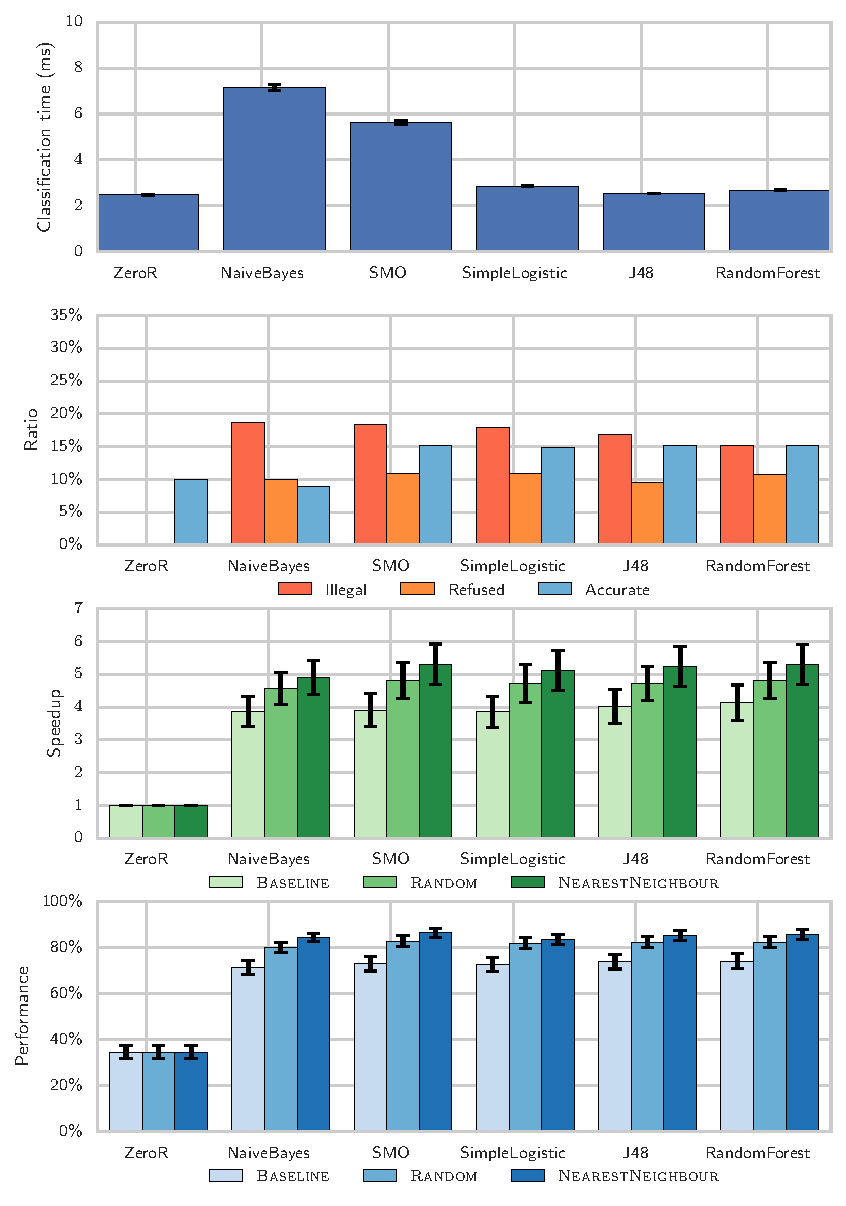
\includegraphics[width=\columnwidth]{img/classification-arch}
\caption[Classification results using cross-device evaluation]{%
  Classification results of cross-device evaluation. Each classifier
  is trained using data from $n-1$ devices, and tested for prediction
  quality using data for the $n^{th}$ device.%
}
\label{fig:class-arch}
\end{figure}

\begin{figure}
\centering
\begin{subfigure}[h]{.45\columnwidth}
\centering
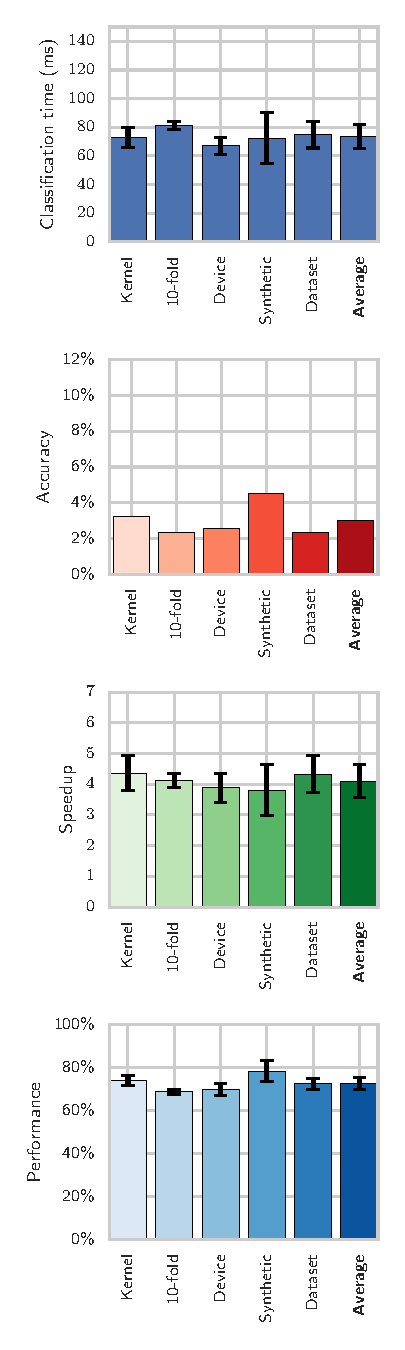
\includegraphics[width=\columnwidth]{img/runtime-class-xval}
\caption{}
\label{fig:runtime-class-xval}
\end{subfigure}
~%
\begin{subfigure}[h]{.45\columnwidth}
\centering
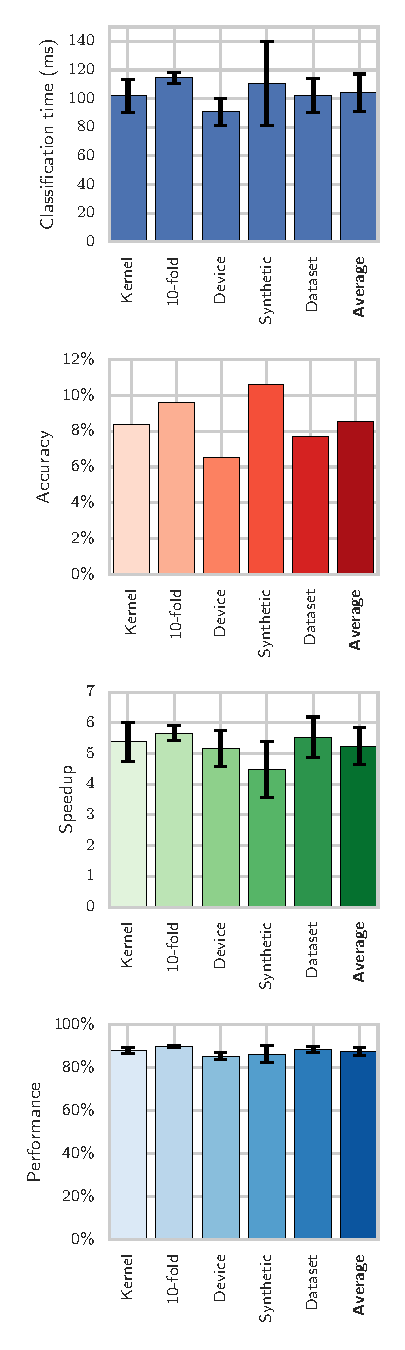
\includegraphics[width=\columnwidth]{img/speedup-class-xval}
\caption{}
\label{fig:speedup-class-xval}
\end{subfigure}
\caption[Autotuning performance using regressors]{%
  Evaluating the effectiveness of classification using regressors, by
  predicting: (\subref{fig:runtime-class-xval}) the workgroup size
  with the minimal runtime, and (\subref{fig:speedup-class-xval}) the
  workgroup size with the greatest speedup over a baseline.%
}
\label{fig:regression-class}
\end{figure}

With the exception of the ZeroR, which predicts \emph{only} the
baseline workgroup size $w_{\left( 4 \times 4 \right)}$, the
classifiers achieve good speedups over the baseline. Average
classification speedups across all validation sets range between
$4.61\times$ and $5.05\times$. Figures~\ref{fig:class-syn}
and~\ref{fig:class-arch} show a summary of results using 10-fold
cross-validation and cross-device validation, respectively.  The
highest average speedup is achieved by SMO, and the lowest by Naive
Bayes. The difference between average speedups is not significant
between the types of classifier, with the exception of SimpleLogistic,
which performs poorly when trained with synthetic benchmarks and
tested against real-world programs. This suggests the model
over-fitting to features of the synthetic benchmarks which are not
shared by the real-world
tests.

\begin{figure}
\centering
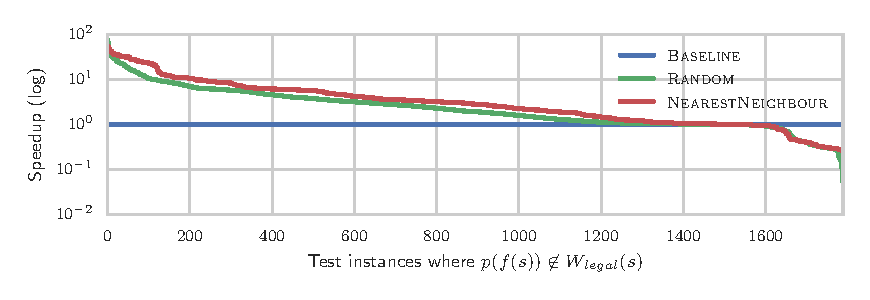
\includegraphics[width=\columnwidth]{img/fallback_speedups}
\caption[Comparison of fallback handler speedups]{%
  Comparison of fallback handlers, showing the speedup over baseline
  parameter for all test cases where a classifier predicted an illegal
  workgroup size.%
}
\label{fig:fallback-speedups}
\end{figure}

By isolating the test cases where classifiers predicted an illegal or
refused parameter, we can directly compare the relative effectiveness
of each fallback handler. The fallback handler with the best average
case performance is \textsc{NearestNeighbour}, with an average speedup
across all classifiers and validation sets of $5.26\times$. The
speedup of \textsc{Random} fallback handler is $3.69\times$, and
$1.0\times$ for \textsc{Baseline}. Figure~\ref{fig:fallback-speedups}
plots the speedups of each fallback handler for all of these isolated
test cases. Interestingly, both the lowest and highest speedups are
achieved by the \textsc{Random} fallback handler, since it essentially
performs a random exploration of the optimisation space. However, the
\textsc{NearestNeighbour} fallback handler provides consistently
greater speedups for the majority of test cases, indicating that it
successfully exploits the structure of the optimisation spaces.

Figures~\ref{fig:runtime-class-xval} and ~\ref{fig:speedup-class-xval}
show a summary of results for classification using regressors to
predict program runtimes and speedups, respectively. Of the two
regression techniques, predicting the \emph{speedup} of workgroup
sizes is much more successful than predicting the \emph{runtime}. This
is most likely caused by the inherent difficulty in predicting the
runtime of arbitrary programs, where dynamic factors such as flow
control and loop bounds are not captured by the kernel features used
in OmniTune, which instead use simple static static instruction counts
and densities. The average speedup achieved by predicting runtimes is
$4.14\times$. For predicting speedups, the average is $5.57\times$.
Tables~\ref{tab:class}, \ref{tab:runtime-class},
and~\ref{tab:speedup-class} show mean performances and speedups for:
J48 classifier using the \textsc{NearestNeighour} fallback strategy,
classification using runtime regression, and classification using
speedup regression, respectively.

If we eliminate the 2.6\% of test cases for which the workgroup size
of $w_{(32 \times 4)}$ is illegal, we can compare the performance of
OmniTune directly against the human expert chosen workgroup
size. Figure~\ref{fig:speedup-distributions} compares the speedups of
all such validation instances over the human expert parameter, for
each autotuning technique. The speedup distributions show consistent
classification results for the five classification techniques, with
the speedup at the lower quartile for all classifiers being
$\ge 1.0\times$. The IQR for all classifiers is $< 0.5$, but there are
outliers with speedups both well below $1.0\times$ and well above
$2.0\times$. In contrast, the speedups achieved using runtime
regression have a lower range, but also a lower median and a larger
IQR. Clearly, runtime regression is the least effective of the
evaluated autotuning techniques. Speedup regression is more
successful, with the highest median speedup of all the
techniques. However, it also has a large IQR and the lower quartile
has a speedup value well below 1, meaning that for more than 25\% of
test instances, the workgroup size selected did not perform as well as
the human expert selected workgroup size.

% The lower average speedup attained by speedup regression over the
% J48 classifier belies the fact that the \emph{median} speedup is
% much greater, at $1.33 \times$.


\begin{figure}
\centering
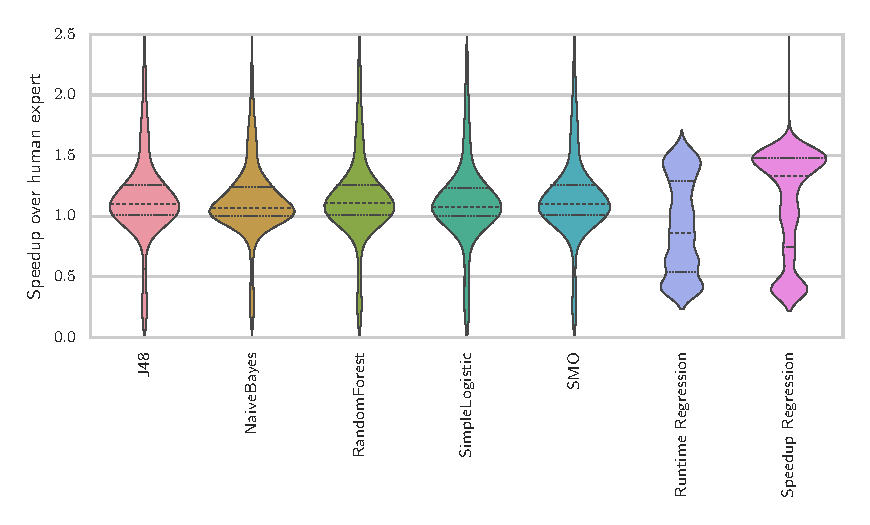
\includegraphics[width=\columnwidth]{img/speedup-distributions}
\caption[Speedup results over human expert]{%
  Distributions of speedups over \emph{human expert}, ignoring cases
  where human expert prediction is invalid. Classifiers are using
  \textsc{NearestNeighbour} fallback handlers. The speedup axis is
  fixed to the range 0--2.5 to highlight the IQRs, which results in
  some outliers > 2.5 being clipped.%
}
\label{fig:speedup-distributions}
\end{figure}


\begin{table}
\scriptsize
\centering
\begin{tabular}{llll}
\toprule
              Job &    Performance &            Speedup &       Human Expert \\
\midrule
          10-fold &           92\% &       $5.65\times$ &       $1.26\times$ \\
        Synthetic &           92\% &       $4.79\times$ &       $1.13\times$ \\
           Device &           85\% &       $5.23\times$ &       $1.17\times$ \\
           Kernel &           89\% &       $5.43\times$ &       $1.21\times$ \\
          Dataset &           91\% &       $5.63\times$ &       $1.25\times$ \\
 \textbf{Average} &  \textbf{90\%} &  $\bm{5.45\times}$ &  $\bm{1.22\times}$ \\
\bottomrule
\end{tabular}
\caption{Validation results for J48 and \textsc{NearestNeighbour}
  classification.}
\label{tab:class}
\end{table}
\begin{table}
\scriptsize
\centering
\begin{tabular}{llll}
\toprule
              Job &    Performance &            Speedup &       Human Expert \\
\midrule
          10-fold &           68\% &       $4.13\times$ &       $0.88\times$ \\
        Synthetic &           78\% &       $3.81\times$ &       $1.06\times$ \\
           Device &           69\% &       $3.89\times$ &       $0.97\times$ \\
           Kernel &           74\% &       $4.36\times$ &       $1.04\times$ \\
          Dataset &           72\% &       $4.33\times$ &       $0.98\times$ \\
 \textbf{Average} &  \textbf{70\%} &  $\bm{4.14\times}$ &  $\bm{0.92\times}$ \\
\bottomrule
\end{tabular}
\caption{Validation results for runtime regression.}
\label{tab:runtime-class}
\end{table}
\begin{table}
\scriptsize
\centering
\begin{tabular}{llll}
\toprule
              Job &    Performance &            Speedup &       Human Expert \\
\midrule
          10-fold &           89\% &       $5.67\times$ &       $1.10\times$ \\
        Synthetic &           86\% &       $4.48\times$ &       $1.19\times$ \\
           Device &           85\% &       $5.18\times$ &       $1.15\times$ \\
           Kernel &           88\% &       $5.38\times$ &       $1.15\times$ \\
          Dataset &           88\% &       $5.53\times$ &       $1.13\times$ \\
 \textbf{Average} &  \textbf{89\%} &  $\bm{5.57\times}$ &  $\bm{1.12\times}$ \\
\bottomrule
\end{tabular}
\caption{Validation results for speedup regression.}
\label{tab:speedup-class}
\end{table}


% \subsubsection{Visualising Prediction Errors}

\begin{figure}
\centering
\begin{subfigure}[t]{0.45\columnwidth}
\centering
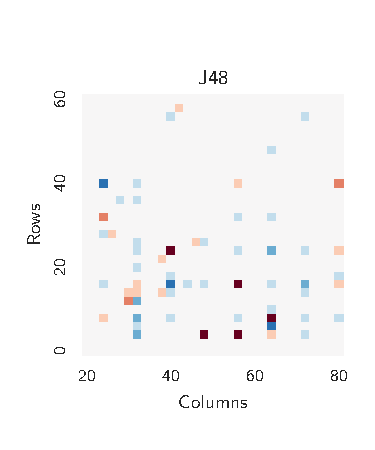
\includegraphics[width=\columnwidth]{img/heatmap_1}
\vspace{-1.5em} % Shrink vertical padding
\caption{}
\label{fig:class-hmaps-1}
\end{subfigure}
~%
\begin{subfigure}[t]{0.45\columnwidth}
\centering
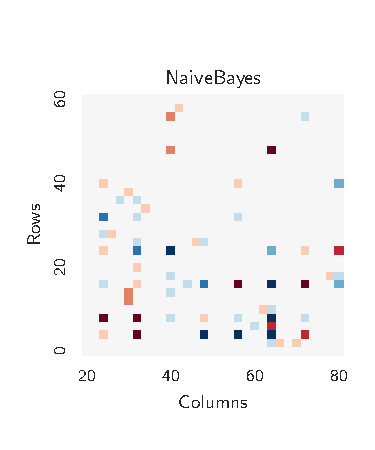
\includegraphics[width=\columnwidth]{img/heatmap_2}
\vspace{-1.5em} % Shrink vertical padding
\caption{}
\label{fig:class-hmaps-2}
\end{subfigure}
\\
\begin{subfigure}[t]{0.45\columnwidth}
\centering
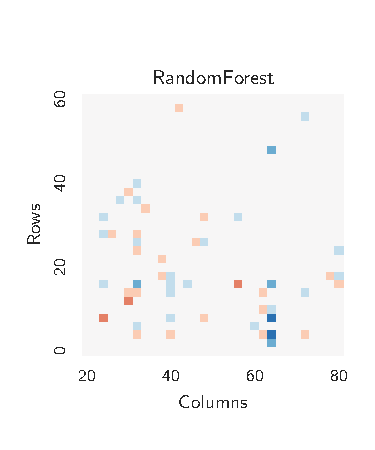
\includegraphics[width=\columnwidth]{img/heatmap_3}
\vspace{-1.5em} % Shrink vertical padding
\caption{}
\label{fig:class-hmaps-3}
\end{subfigure}
~%
\begin{subfigure}[t]{0.45\columnwidth}
\centering
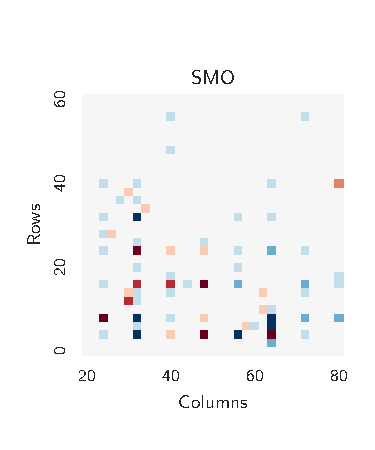
\includegraphics[width=\columnwidth]{img/heatmap_5}
\vspace{-1.5em} % Shrink vertical padding
\caption{}
\label{fig:class-hmaps-4}
\end{subfigure}
\\
\begin{subfigure}[t]{0.45\columnwidth}
\centering
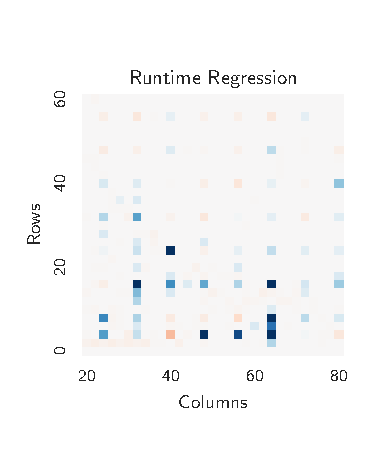
\includegraphics[width=\columnwidth]{img/reg_runtime_heatmap}
\vspace{-1.5em} % Shrink vertical padding
\caption{}
\label{fig:class-hmaps-5}
\end{subfigure}
~%
\begin{subfigure}[t]{0.45\columnwidth}
\centering
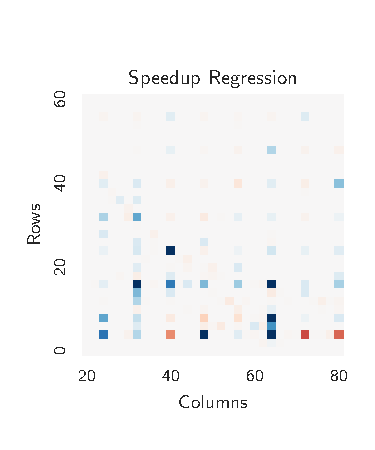
\includegraphics[width=\columnwidth]{img/reg_speedup_heatmap}
\vspace{-1.5em} % Shrink vertical padding
\caption{}
\label{fig:class-hmaps-6}
\end{subfigure}
\caption[Classification error heatmaps]{%
  Heatmaps of classification errors for 10-fold cross-validation,
  showing a subset of the optimisation space. The shading in each
  cells indicates if it is predicted less frequently (blue), ore more
  frequently (red) than it is optimal. Colour gradients are normalised
  across plots.%
}
\label{fig:class-hmaps}
\end{figure}


The prediction costs using regression are significantly greater than
using classifiers. This is because, while a classifier makes a single
prediction, the number of predictions required of a regressor grows
with the size of $W_{\max}(s)$, since classification with regression
requires making predictions for all
$w \in \left\{ w | w < W_{\max}(s) \right\}$. The fastest classifier
is J48, due to the it's simplicity (it can be implemented as a
sequence of nested \texttt{if}/\texttt{else} statements).

Figure~\ref{fig:class-hmaps} visualises the classification errors of
each of the autotuning techniques. It shows that while the performance
of all of the classifiers is comparable, the distribution of
predictions is not. Only the NaiveBayes and RandomForest classifiers
predicted the human expert selected workgroup size of
$w_{(32 \times 4)}$ as frequently, or more frequently, than it was
optimal. The two regression techniques were the least accurate of all
of the autotuning techniques.


\subsubsection{Summary}

From an evaluation of 17 different autotuning techniques using 5
different types of validation sets, the following conclusions about
autotuning performance can be drawn:
%
\begin{itemize}
\item In the case of classifiers predicting illegal workgroup sizes,
  the best fallback strategy is to select the closest legal workgroup
  size.
\item The performance of predicted workgroup sizes for unseen devices
  is within 8\% of the performance for known devices.
\item Predicting the \emph{runtime} of stencils is the least effective
  of the evaluated autotuning techniques, achieving an average of only
  68\% of the available performance.
\item Predicting the \emph{speedup} of workgroup sizes provides the
  highest median speedup, but more frequently predicts a poorly
  performing workgroup size then the classifiers.
\item Classification using regression costs an order of magnitude more
  time than using classifiers. The J48 classifier has the lowest
  overhead.
\end{itemize}



\section{Conclusions}\label{sec:conclusions}

As the trend towards higher core counts and increasing parallelism
continues, the need for high level, accessible abstractions to manage
such parallelism will continue to go. Autotuning proves a valuable aid
for achieving these goals, providing the benefits of low level
performance tuning while maintaining ease of use, without burdening
developers with optimisation concerns. As the need for autotuned
parallelism rises, the desire for collaborative techniques for sharing
performance data must be met with systems capable of supporting this
cross-platform learning.

In this thesis, I have presented my attempt at providing such a
system, by designing a novel framework which has the benefits of fast,
``always-on'' autotuning, while being able to synchronise data with
global repositories of knowledge which others may contribute to. The
framework provides an interface for autotuning which is sufficiently
generic to be easily re-purposed to target a range of optimisation
parameters.

To demonstrate the utility of this framework, I implemented a frontend
for predicting the workgroup size of OpenCL kernels for SkelCL stencil
codes. This optimisation space is complex, non linear, and critical
for the performance of stencil kernels, with up to a $207.72\times$
slowdown if an improper value is picked. Selecting the correct
workgroup size is difficult --- requiring a knowledge of the kernel,
dataset, and underlying architecture. The challenge is increased even
more so by inconsistencies in the underlying system which cause some
workgroup sizes to fail completely. Of the 269813 combinations of
workgroup size, device, program, and dataset tested; only a
\emph{single} workgroup size was valid for all test cases, and
achieved only 24\% of the available performance. The value selected by
human experts was invalid for 2.6\% of test cases. Autotuning in this
space requires a system which is resilient these challenges, and
several techniques were implemented to address them.

Runtime performance of autotuned stencil kernels is very promising,
achieving an average 90\% of the available performance with only a 3ms
autotuning overhead. Even ignoring the cases for which the human
expert selected workgroup size is invalid, this provides a
$1.33\times$ speedup, or a $5.57\times$ speedup over the best
performance that can be achieved using static tuning. Classification
performance is comparable when predicting workgroup sizes for both
unseen programs and unseen devices. I believe that the combination of
performance improvements and the collaborative nature of OmniTune
makes for a compelling case for the use of autotuning as a key
component for enabling performant, high level parallel programming.


\subsection{Critical Analysis}

This subsection contains a critical analysis of the work presented in
previous sections.

\paragraph{OmniTune Framework}

The purpose of the OmniTune framework is to provide a generic
interface for runtime autotuning. This is demonstrated through the
implementation of a SkelCL frontend; however, to truly evaluate the
ease of use of this framework, it would have been preferable to
implement one or more additional autotuning frontends, to target
different optimisation spaces. This could expose any leakages in the
abstractions between the SkelCL-specific and generic autotuning
components.


\paragraph{Synthetic Benchmarks}

The OmniTune SkelCL frontend provides a template substitution engine
for generating synthetic stencil benchmarks. The implementation of
this generator is rigidly tied to the SkelCL stencil format. It would
be preferred if this template engine was made more flexible, to
support generation of arbitrary test programs. Additionally, due to
time constraints, I did not have the opportunity to explore how the
number of synthetic benchmarks in machine learning test data sets
affects classification performance.

One possible use of the synthetic stencil benchmark generator could be
for creating minimal test cases of refused OpenCL parameters so that
bug reports could be filed with the relevant implementation
vendor. However, this would have added a great level of complexity to
the the generator, as it would have to isolate and remove the
dependency on SkelCL to generate minimal programs, requiring
significant implementation work.


\paragraph{Use of Machine Learning}

The evaluation of OmniTune in this thesis uses multiple classifiers
and regressors to predict workgroup sizes. The behaviour of these
classifiers and regressors is provided by the Weka data mining
suite. Many of these classifiers have parameters which affect their
prediction behaviour. The quality of the evaluation could have been
improved by exploring the effects that changing the values of these
parameters has on the OmniTune classification performance. It would
also have been informative to dedicate a portion of the evaluation to
feature engineering, evaluating the information gain of each feature
and exploring the effects of feature transformations on classification
performance.


\paragraph{Evaluation Methodology}

The evaluation compares autotuning performance against the best
possible performance that can be achieved using static tuning, a
simple heuristic to tune workgroup size on a per-device basis, and
against the workgroup size chosen by human experts. It would have been
beneficial to also include a comparison of the performance of these
autotuned stencils against hand-crafted equivalent programs in pure
OpenCL, without using the SkelCL framework. This would allow a direct
comparison between the performance of stencil kernels using high level
and low level abstractions, but could not be completed due to time
constraints and difficulties in acquiring suitable comparison
benchmarks and datasets.


\subsection{Future Work}

Future work can be divided into two categories: continued development
of OmniTune, and extending the behaviour of the SkelCL autotuner.

The cost of offline training with OmniTune could be reduced by
exploring the use of adaptive sampling plans, such as presented
in~\cite{Leather2009}. This could reduce the number of runtime samples
required to distinguish good from bad optimisation parameter values.

Algorithm~\ref{alg:autotune-hybrid} proposes the behaviour of a hybrid
approach to selecting the workgroup size of iterative SkelCL
stencils. This approach attempts to exploit the advantages of all of
the techniques presented in this thesis. First, runtime regression is
used to predict the minimum runtime and a candidate workgroup
size. If, after evaluating this workgroup size, the predicted runtime
turned out to be inaccurate, then a prediction is made using speedup
regression. Such a hybrid approach would enable online tuning through
the continued acquisition of runtime and speedup performance, which
would compliment the collaborative aspirations of OmniTune, and the
existing server-remote infrastructure.

Other skeleton optimisation parameters could be autotuned by SkelCL,
including higher level optimisations such as the selection of border
region loading strategy, or selecting the optimal execution device(s)
for multi-device systems. Optimisation parameters of additional
skeletons could be autotuned, or the interaction of multiple related
optimisation parameters could be explored. Power consumption could be
used as an additional optimisation cotarget.

\begin{algorithm}
\begin{algorithmic}[1]
\Require kernel features $k$, hardware features $h$, dataset features $d$.
\Ensure workgroup size $w$

\State $r \leftarrow \underset{w \in W_{legal}(s)}{\min} f(k,h,d,w)$
\Comment Predict minimum runtime.
\State $w \leftarrow \underset{w \in W_{legal}(s)}{\argmin} f(k,h,d,w)$
\Comment Workgroup size for $r$.
\State $t_r \leftarrow$ measure runtime of program with $w$
\State \textsc{Submit}$\left( f(s), w, t_r \right)$
\Comment Submit observed runtime
\If{$t_r \approx r$}
  \State \textbf{return} $w$
\Comment Predicted runtime is accurate.
\Else
   \State $W \leftarrow \left\{ w | w < W_{\max}(s) \right\}$
   \State converged $\leftarrow$ false
   \State $w_b \leftarrow$ baseline parameter
   \State $t_b \leftarrow$ measure runtime of runtime of program with
   $w_b$
   \State \textsc{Submit}$\left( f(s), w_b, t_b \right)$
   \Comment Submit observed runtime
   \While{not converged}
     \State $s \leftarrow \underset{w \in W}{\max} g(k,h,d,w)$
     \Comment Predict best speedup.
     \State $w \leftarrow \underset{w \in W}{\argmax} g(k,h,d,w)$
     \Comment Workgroup size for $s$.
     \State $t \leftarrow$ measure runtime of program with $s$
     \State \textsc{Submit}$\left( f(s), w, t \right)$
     \Comment Submit observed runtime
     \State $s_w \leftarrow t_t / t$
     \State \textsc{Submit}$\left( f(s), w, s_w \right)$
     \Comment Submit observed speedup
     \If{$s_w \approx s$}
       \State converged = true
       \Comment Predicted speedup is accurate.
     \Else
       \State $W = W - \{ w \}$
     \EndIf
   \EndWhile
   \State \textbf{return} $w$
\EndIf
\end{algorithmic}
\caption{%
  Selecting workgroup size using a combination of classifiers and
  regressors.%
}
\label{alg:autotune-hybrid}
\end{algorithm}



%
% \appendix
% \section{Appendix Title}
%
% This is the text of the appendix, if you need one.
%

\acks

This work was supported by grant EP/L01503X/1 for the University of
Edinburgh School of Informatics Centre for Doctoral Training in
Pervasive Parallelism (\url{http://pervasiveparallelism.inf.ed.ac.uk/}) from
the UK Engineering and Physical Sciences Research Council (EPSRC).

% We recommend abbrvnat bibliography style.

\label{bibliography}
\printbibliography


\end{document}
